% !TeX root = ../main.tex

% Slides
\section{Visão geral}
\begin{frame}[c]{Visão geral}
    \begin{columns}[c]
        \begin{column}{0.48\linewidth}
            \begin{splusbox}{}
                \begin{itemize}
                    \item Introdução
                    \begin{itemize}
                        \item Galáxias anãs ultra-compactas (UCDs)
                        \item Galáxias compactas com emissão
                    \end{itemize}
                    \item Dados
                    \begin{itemize}
                        \item Fotometria S-PLUS
                        \item Correções e cortes de qualidade
                        \item Distribuição das UCDs
                    \end{itemize}
                \end{itemize}
            \end{splusbox}
        \end{column}
        %
        \begin{column}{0.48\linewidth}
            \begin{splusbox}{}
                \begin{itemize}
                    \item Aprendizado de máquina
                    \item Seleção das candidatas
                    \item Observações espectroscópicas
                    \item Objetos compactos com emissão
                    \item Conclusões e perspectivas
                \end{itemize}
            \end{splusbox}
        \end{column}
    \end{columns}
\end{frame}

\section{Introdução}


\begin{frame}[c]{O que são UCDs?}
    \begin{itemize}
        \item Galáxias anãs ultra-compactas (UCDs)
        \item Objetos intermediários entre galáxias anãs e aglomerados globulares
        \item Descobertas em aglomerados como Fornax e Virgo
        \item Propriedades:
        \begin{itemize}
            \item Massas: $10^6$ a $10^8$ $M_\odot$
            \item Raios: 7 a 100 pc
            \item Populações estelares antigas
        \end{itemize}
    \end{itemize}
    \vspace{0.5cm}
    \centering
    % 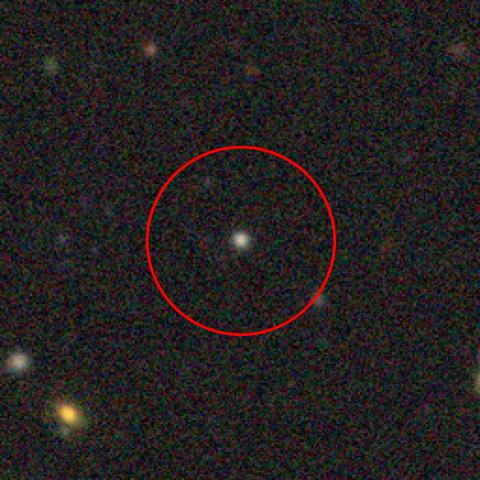
\includegraphics[width=0.5\textwidth]{Images/ucds_exp/UCD_M60.png}
    % Espaço para imagem de UCD
\end{frame}

% Slide 2: Formação e Cenários Evolutivos das UCDs
\begin{frame}[c]{Formação das UCDs}
    \begin{itemize}
        \item Possíveis origens:
        \begin{itemize}
            \item Núcleos remanescentes de galáxias anãs despojadas
            \item Aglomerados globulares massivos
        \end{itemize}
        \item Diversidade de propriedades sugere múltiplos canais de formação
    \end{itemize}
    \vspace{0.5cm}
    \centering
    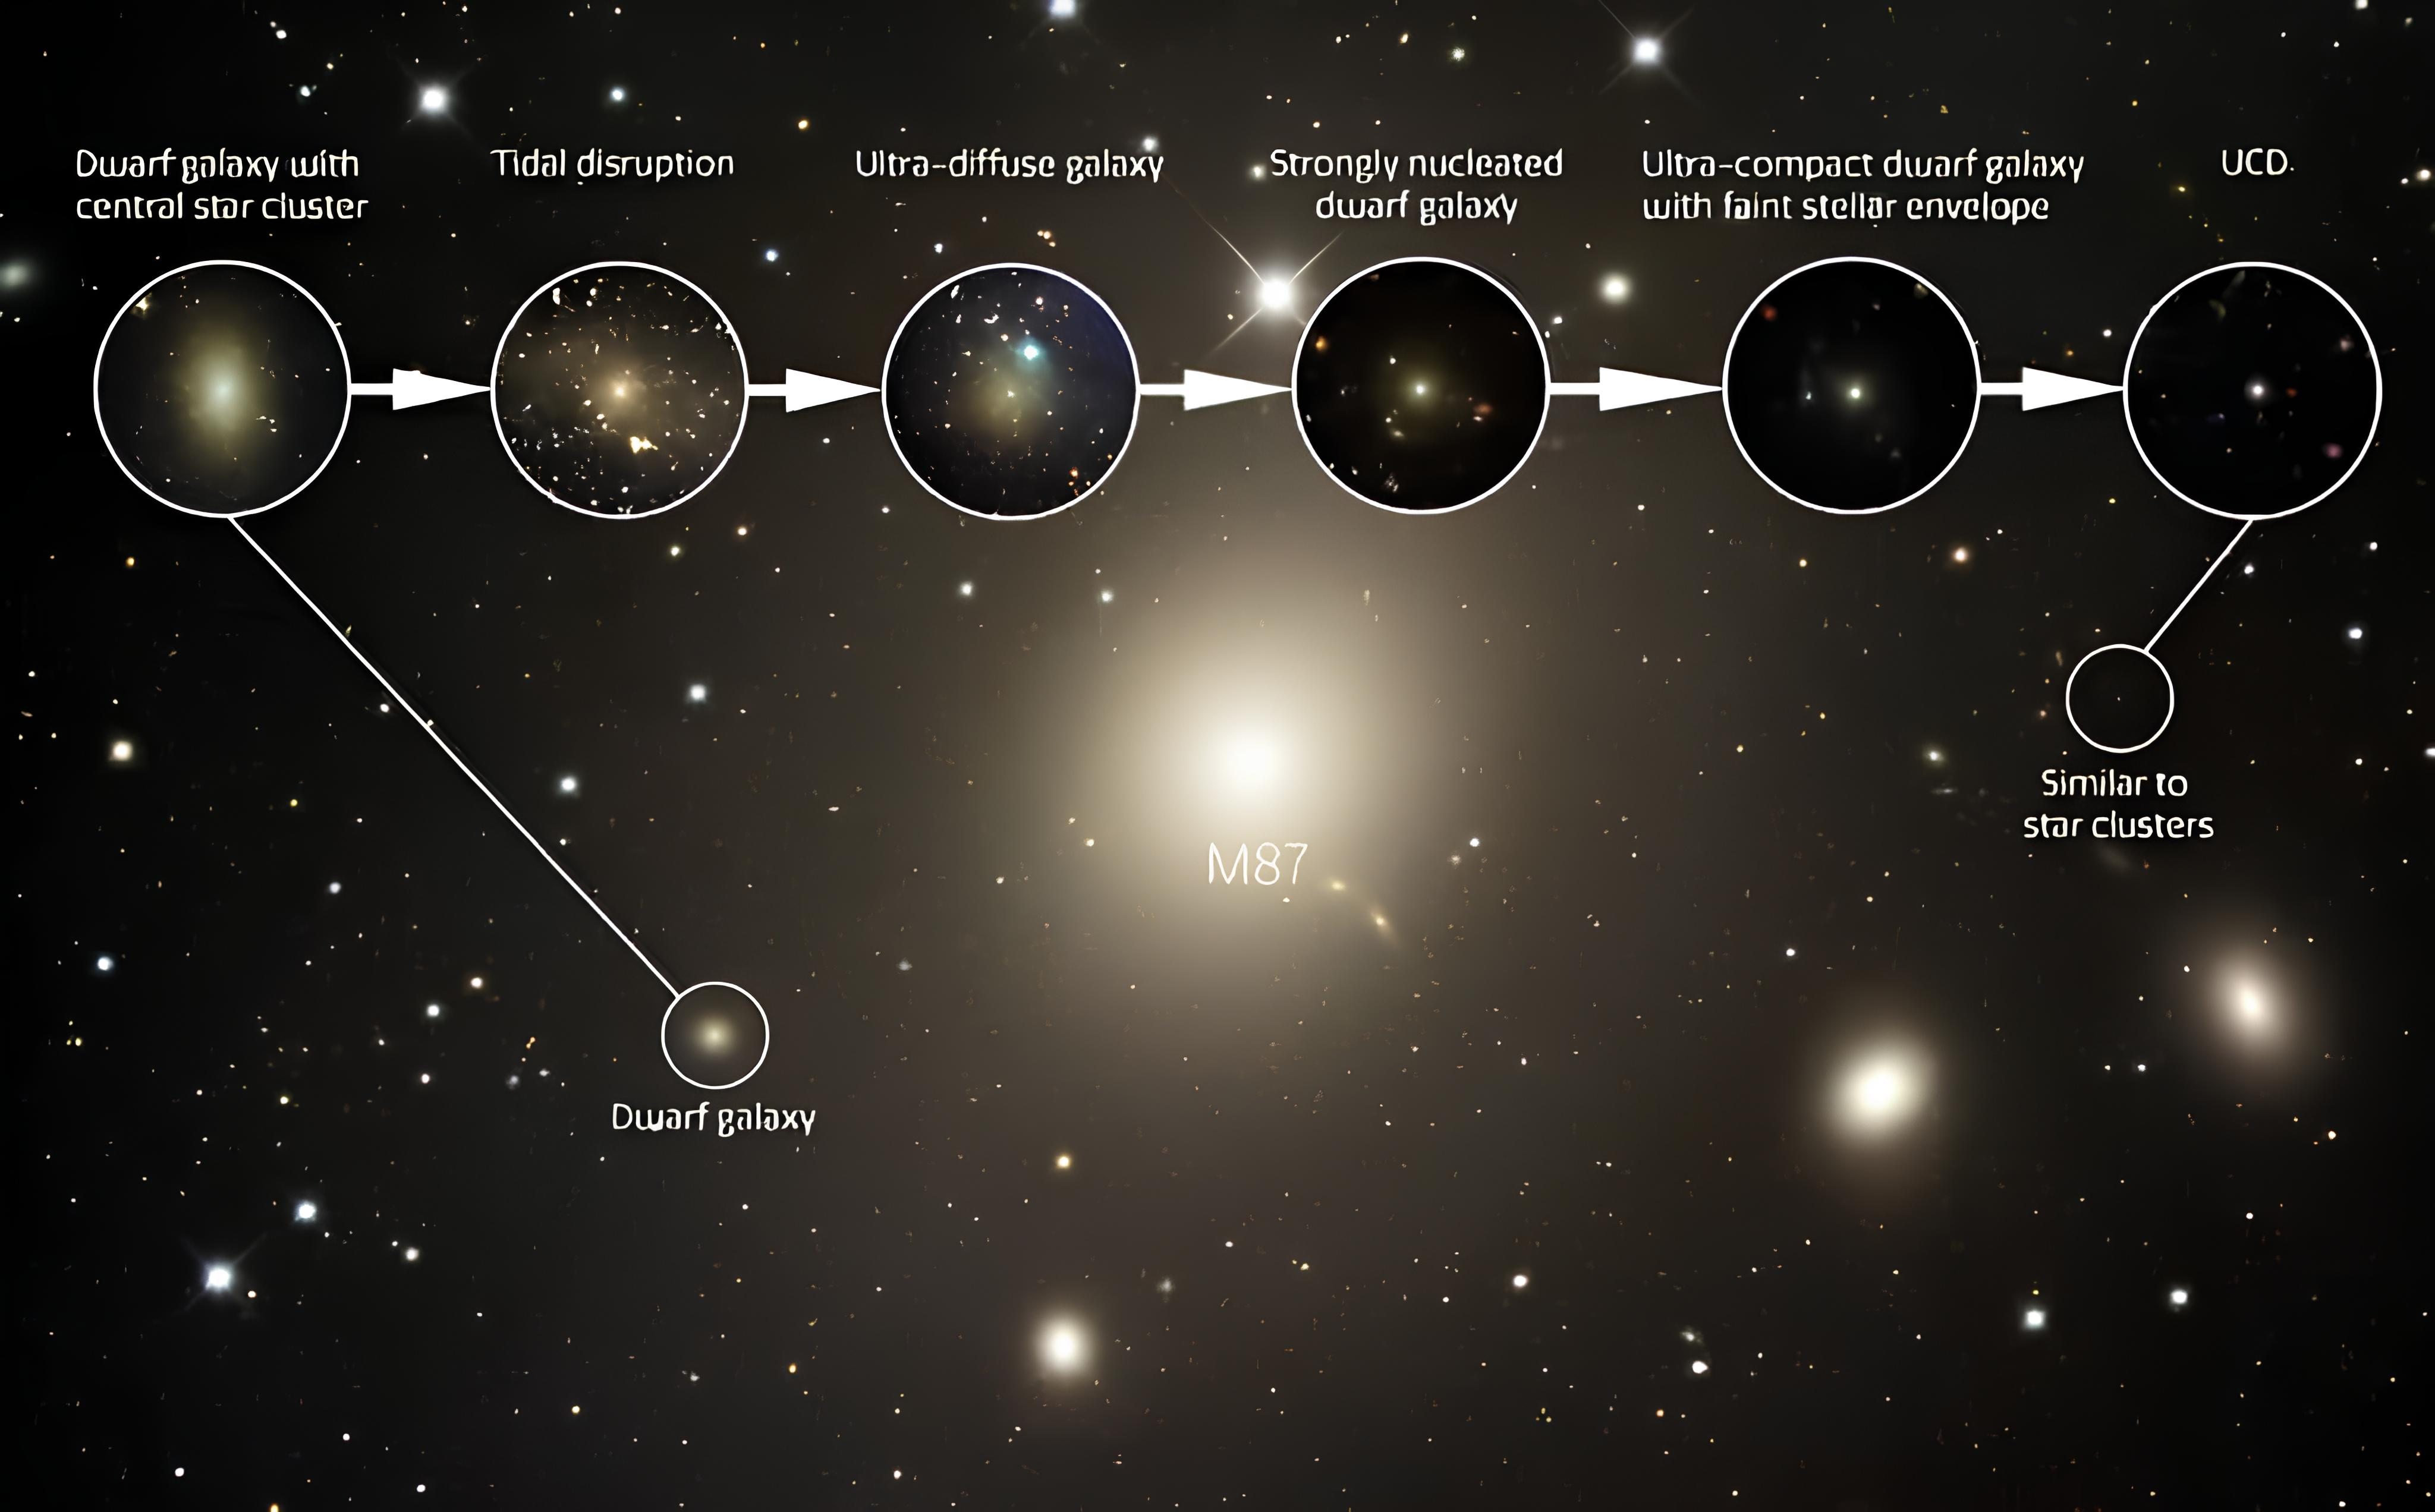
\includegraphics[width=0.4\textwidth]{images/continuo_evolution_dwarf.png}
\end{frame}

\begin{frame}[c]{Galáxias compactas com emissão}
    \begin{itemize}
        \item Exemplos: BCDs (Blue Compact Dwarfs), Green Peas
        \item Características:
        \begin{itemize}
            \item Ricas em gás
            \item Intensos surtos de formação estelar
            \item Espectros dominados por linhas de emissão (H$\alpha$, [OIII], etc.)
        \end{itemize}
        \item Análogas locais de galáxias do universo primordial
    \end{itemize}
    \vspace{0.5cm}
    \centering
    % 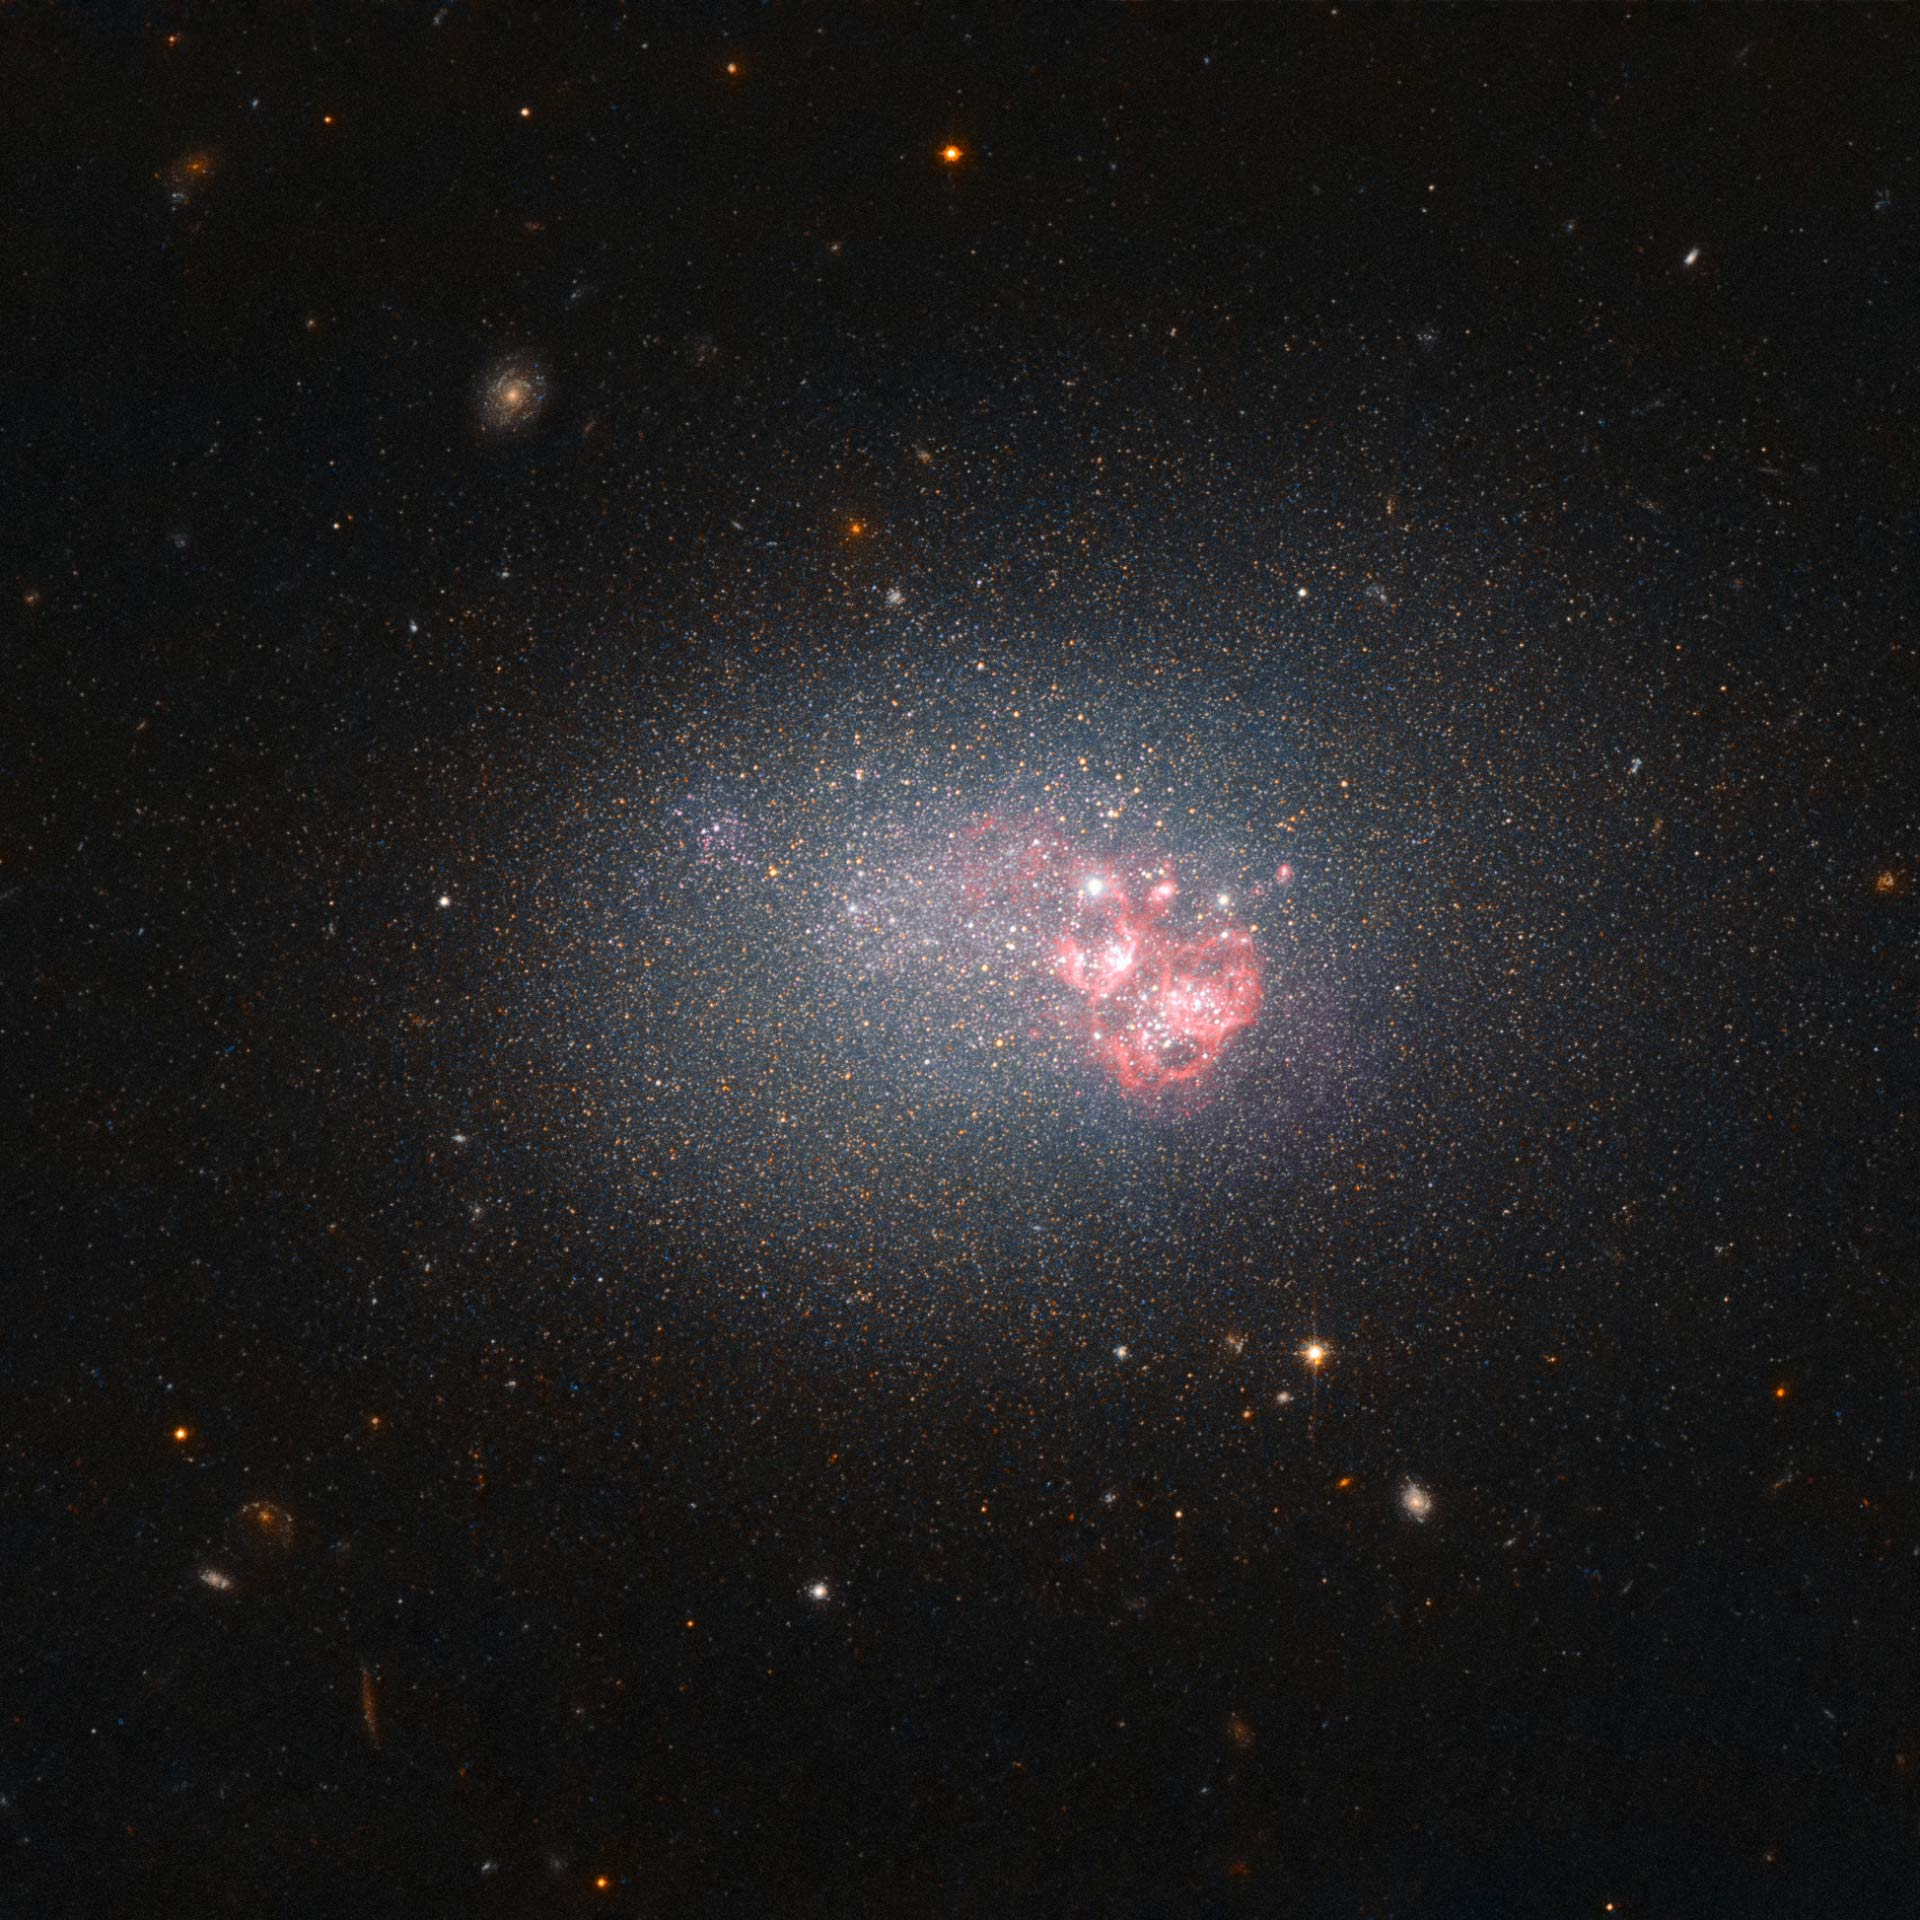
\includegraphics[width=0.4\textwidth]{indroduction/BCD.png}
\end{frame}

\begin{frame}{UCDs vs. Galáxias com emissão}
    \begin{columns}
        \column{0.5\textwidth}
        \textbf{UCDs}
        \begin{itemize}
            \item Espectros dominados por linhas de absorção
            \item Populações estelares antigas
            \item Pouca ou nenhuma formação estelar atual
        \end{itemize}
        \column{0.5\textwidth}
        \textbf{Galáxias compactas com emissão}
        \begin{itemize}
            \item Espectros dominados por linhas de emissão
            \item Formação estelar ativa
            \item Baixa metalicidade
        \end{itemize}
    \end{columns}
\end{frame}


% \begin{frame}[c]{O contexto cosmológico}
%     \begin{splusbox}{}
%         Estudar a formação e evolução da estrutura em larga escala (LSS) é fundamental para entender o Universo em que vivemos. A partir dela podemos ter insights sobre:
%         \begin{itemize}
%             \item Matéria escura
%             \item Energia escura
%             \item Evolução cósmica
%             \item Formação e evolução de galáxias
%             \item Física a nível fundamental
%         \end{itemize}
%     \end{splusbox}
% \end{frame}

% \begin{frame}[c]{Estrutura em larga escala}
%     A teia cósmica, ou a LSS, é formada por diferentes componentes. Cada componente apresenta caracteristicas e possui papéis diferentes na evolução do Universo como um todo.

%     \begin{figure}
%         \centering
%         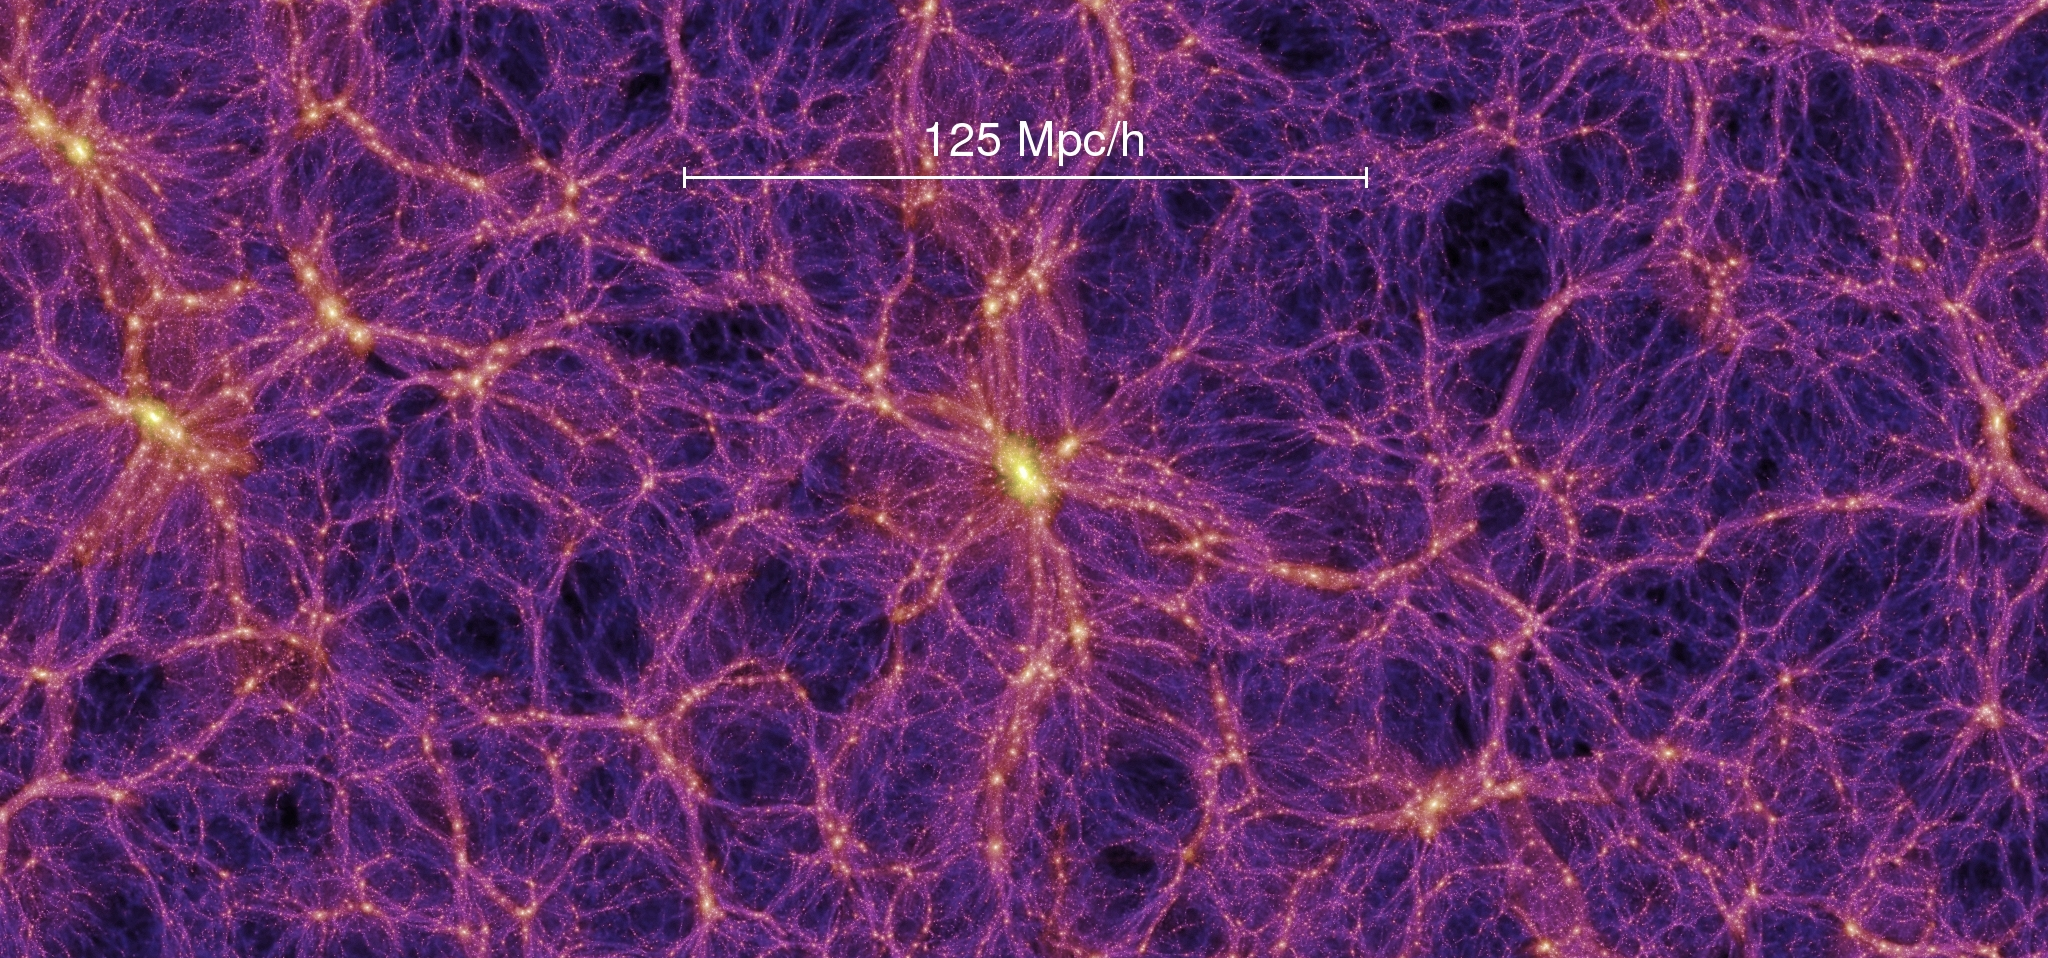
\includegraphics[height=5cm]{script/images/millenium.png}
%         \caption{Adaptado de \url{https://wwwmpa.mpa-garching.mpg.de/galform/virgo/millennium/}.}
%     \end{figure}

%     % \begin{columns}
%     %     \begin{column}{0.32\linewidth}
%     %         \begin{splusbox}{Filamentos}
                
%     %         \end{splusbox}
%     %     \end{column}
%     %     %
%     %     \begin{column}{0.32\linewidth}
%     %         \begin{splusbox}{Aglomerados}
                
%     %         \end{splusbox}
%     %     \end{column}
%     %     %
%     %     \begin{column}{0.32\linewidth}
%     %         \begin{splusbox}{Vazios}
                
%     %         \end{splusbox}
%     %     \end{column}
%     % \end{columns}
% \end{frame}

% \begin{frame}[c]{Estrutura em larga escala}
%     \begin{figure}
%         \centering
%         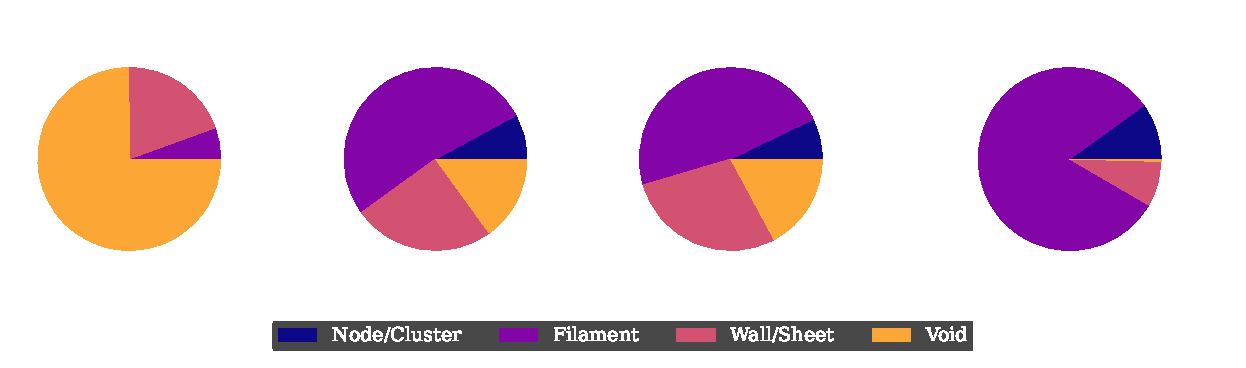
\includegraphics[width=\linewidth]{script/images/lss_distribution.pdf}
%         \caption{Adaptado de: Ganeshaiah Veena et al. (2019).}
%     \end{figure}
% \end{frame}

% \begin{frame}[c]{Estrutura em larga escala}
%     \begin{columns}[c]
%         \begin{column}{0.56\textwidth}
%             \begin{figure}
%                 \centering
%                 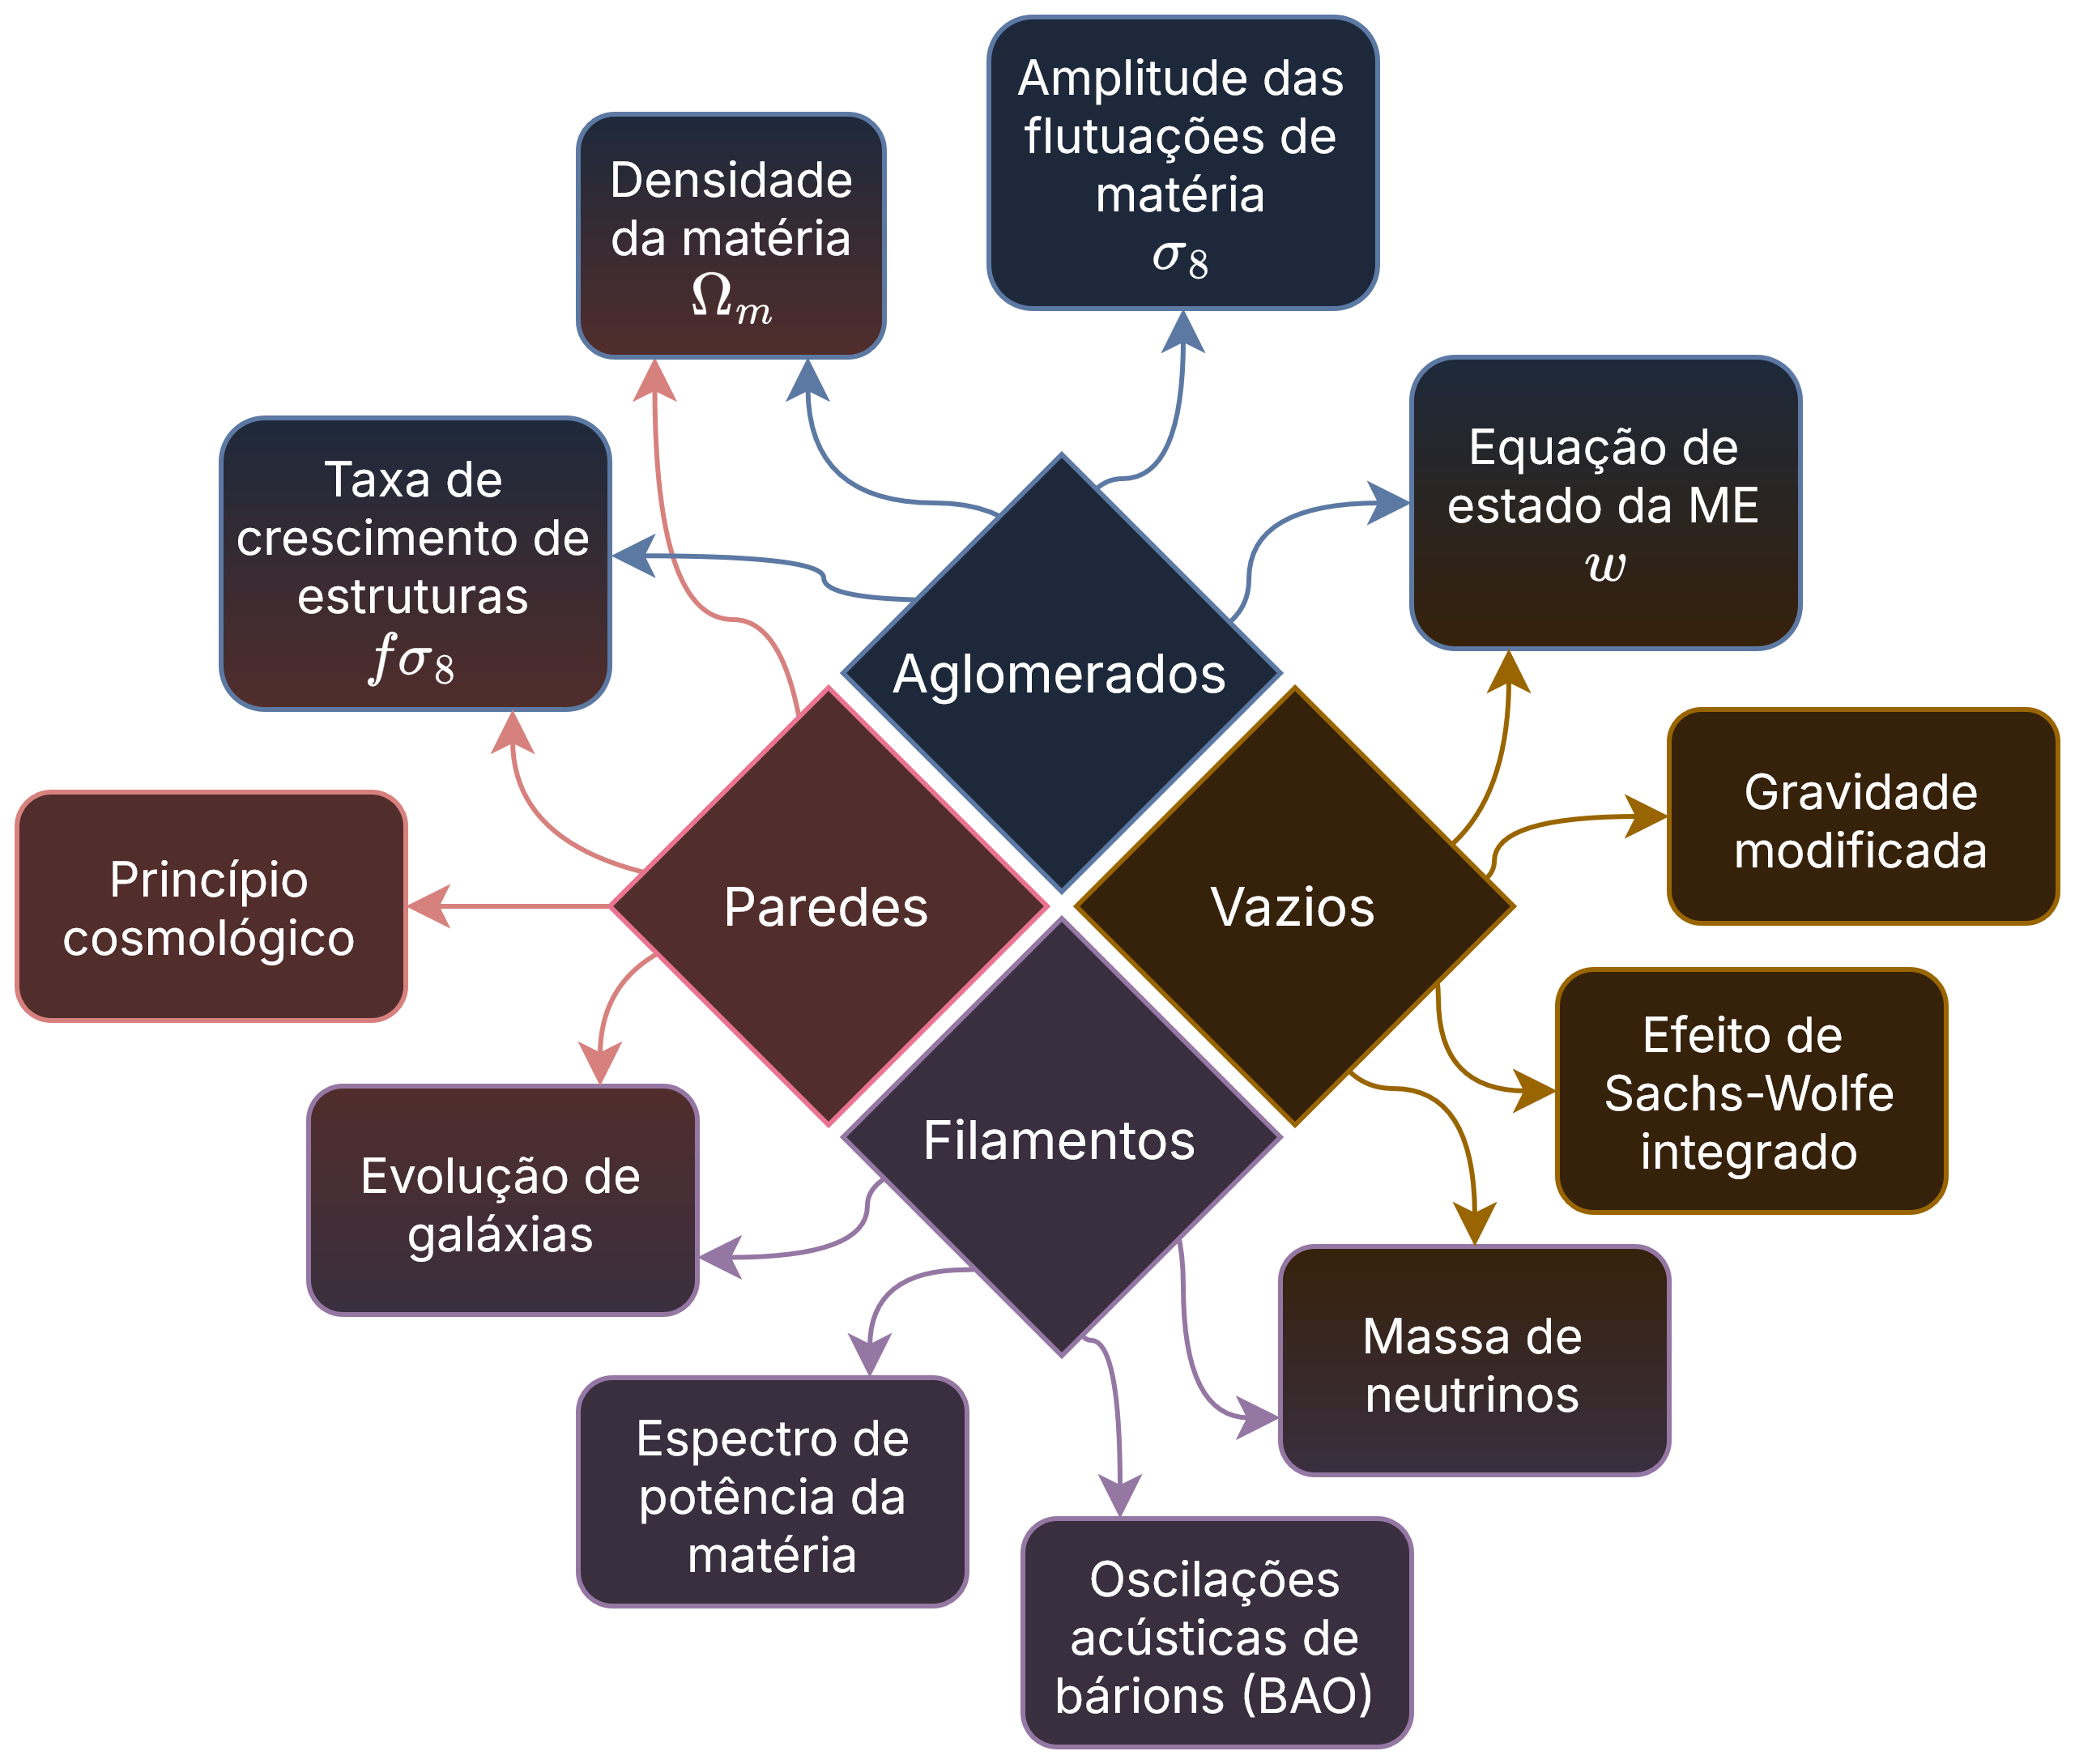
\includegraphics[height=7cm]{images/LSS.png}
%             \end{figure}
%         \end{column}
%         %
%         \begin{column}{0.36\textwidth}
%             \begin{splusbox}{}
%                 O problema é que estas estruturas são tridimensionais, mas nossas observações são projetadas (bidimensionais)
%             \end{splusbox}
%         \end{column}
%     \end{columns}
% \end{frame}


% \begin{frame}[c]{Redshifts espectroscópicos e suas limitações}
%     Uma forma de determinar a distância de objetos celestes vêm da lei de Hubble Lemaître (válida para objetos próximos):
%     \vspace*{-0.5cm}
%     \begin{figure}
%         \centering
%         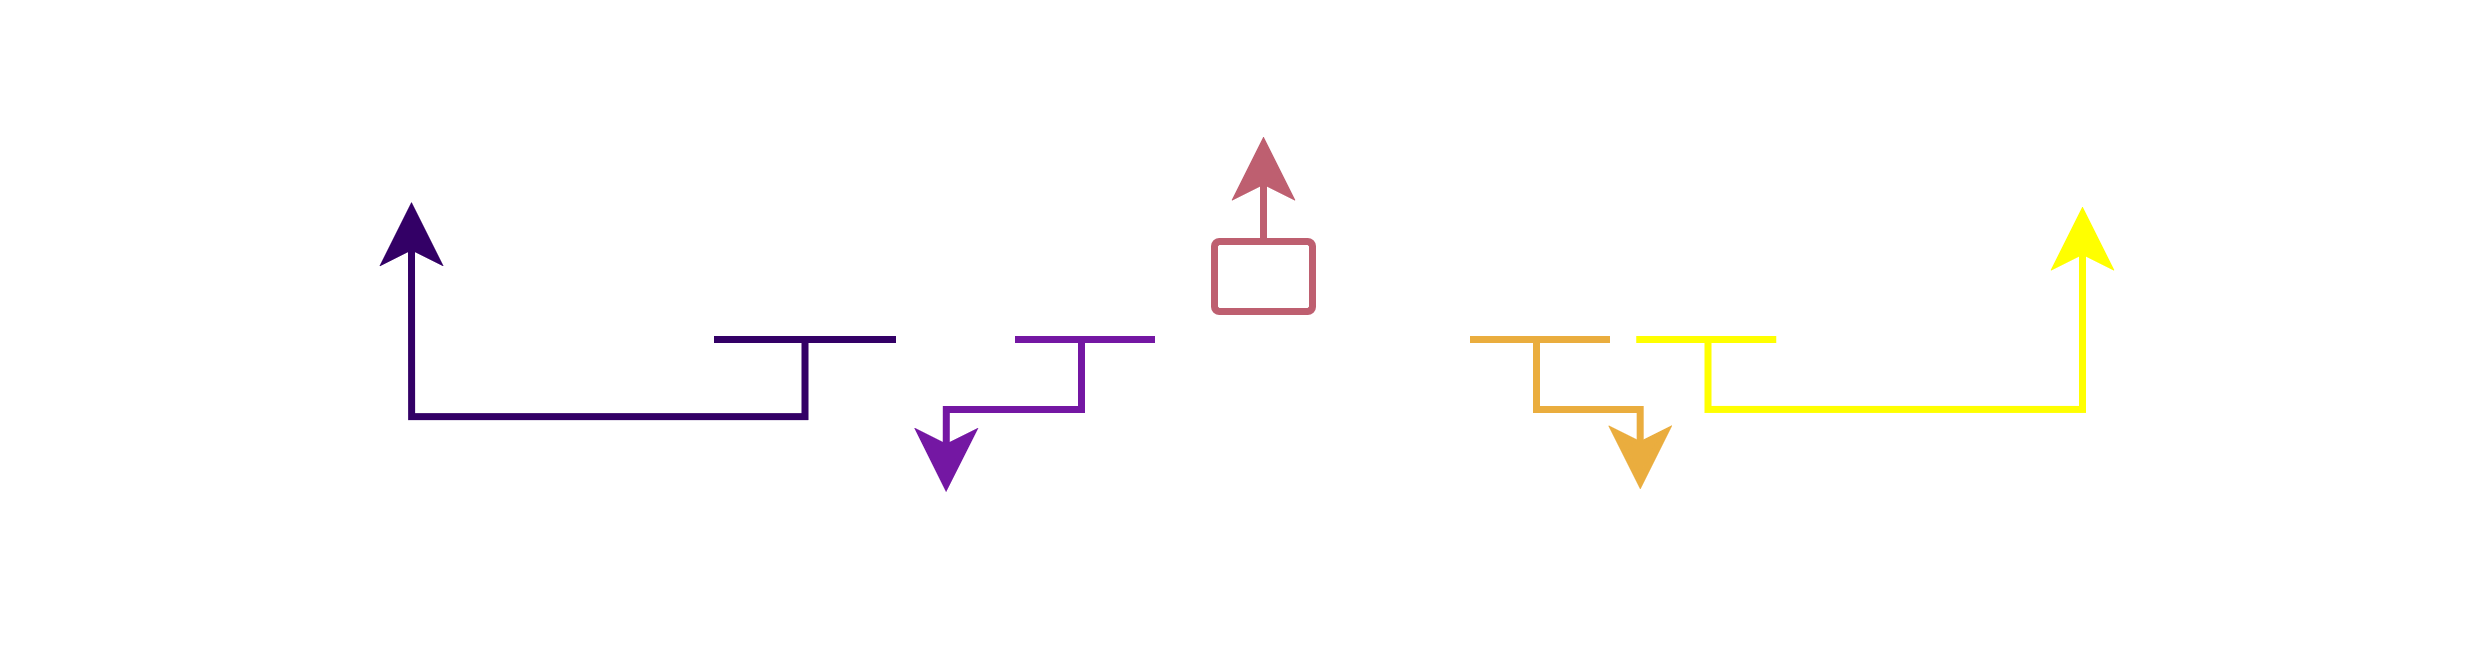
\includegraphics[width=0.8\linewidth]{script/images/hubble_law.png}
%     \end{figure}
%     \vspace*{-0.5cm}
%     \begin{splusbox}{}
%         \centering
%         A observação de um espectro com alto sinal ruído demanda bastante tempo de observação, ainda mais para objetos fracos

%         \vspace{0.3cm}
%         É necessário encontrar uma alternativa
%     \end{splusbox}
% \end{frame}

% \section{O objetivo}
% \begin{frame}[c]{O objetivo}
%     \begin{columns}[c]
%         \begin{column}{0.46\linewidth}
%             \begin{splusbox}{Redshifts fotométricos}
%                 \begin{itemize}
%                     \justifying
%                     \item Determinação de redshifts fotométricos de alta precisão
%                     \item Funções de densidade de probabilidade bem calibradas
%                     \item Galáxias até $z=0.8$ e magnitude 21 na banda \texttt{r}
%                 \end{itemize}
%             \end{splusbox}
%         \end{column}
%         \begin{column}{0.46\linewidth}
%             \begin{splusbox}{Estrutura em larga escala}
%                 \begin{itemize}
%                     \justifying
%                     \item Utilizar dados fotométricos para a reconstrução da LSS
%                     \item Obter um mapeamento similar ao visto usando $z_\text{spec}$
%                     %\item Possibilitar estudos que abrangem diferentes áreas da cosmologia
%                 \end{itemize}
%                 %Recuperação das estrutura da LSS, tal como vemos usando $z_\text{spec}$, a partir de estimativas fotométricas
%             \end{splusbox}
%         \end{column}
%     \end{columns}

%     \centering
%     \begin{splusbox}{}
%         Expandir o conjunto de dados que podemos usar para estudos em diferentes áreas da astronomia
%     \end{splusbox}
% \end{frame}

\section{Dados}

\begin{frame}[c]{Dados fotométricos}
    \begin{figure}
        \centering
        \begin{minipage}{0.48\textwidth}
            \centering
            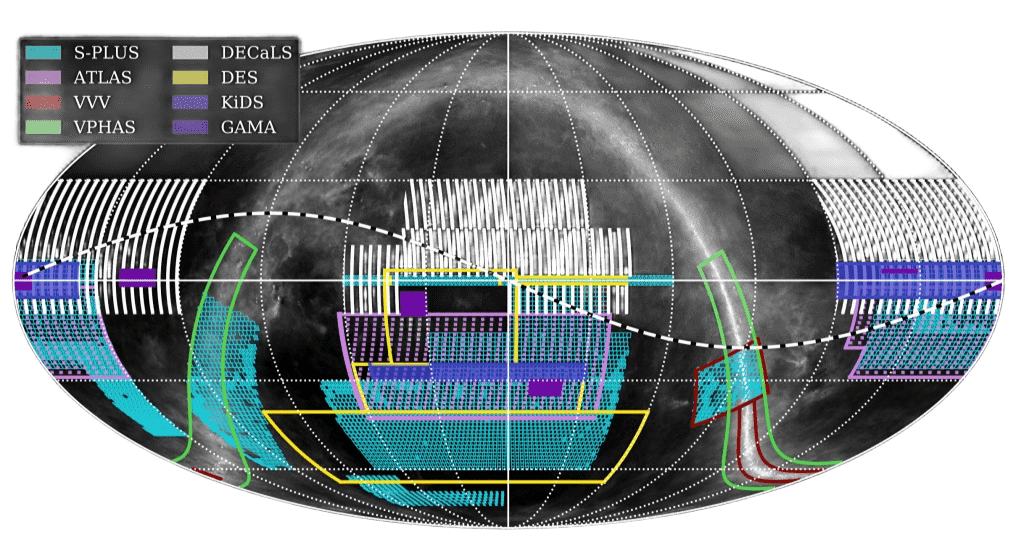
\includegraphics[width=\textwidth]{images/splus_survey_area.png}
            % \caption{}
        \end{minipage}
        \hfill
        \begin{minipage}{0.48\textwidth}
            \centering
            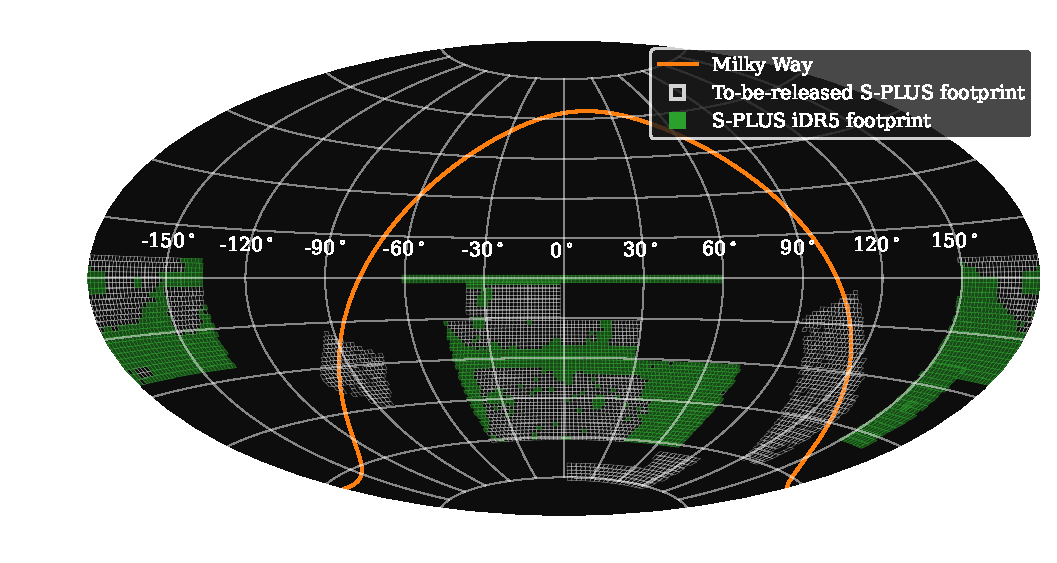
\includegraphics[width=\textwidth]{script/images/splus_footprint_idr5.pdf}
            % \caption{}
        \end{minipage}
    \end{figure}
\end{frame}

\begin{frame}[c]{Dados fotométricos}%[label=current]
    \textbf{DR4}: 3022,7 square degrees,\\
    \textbf{1629} Fields (each $\sim$2 square degrees)\\
    \textbf{Filters}
    \begin{figure}
        \centering
        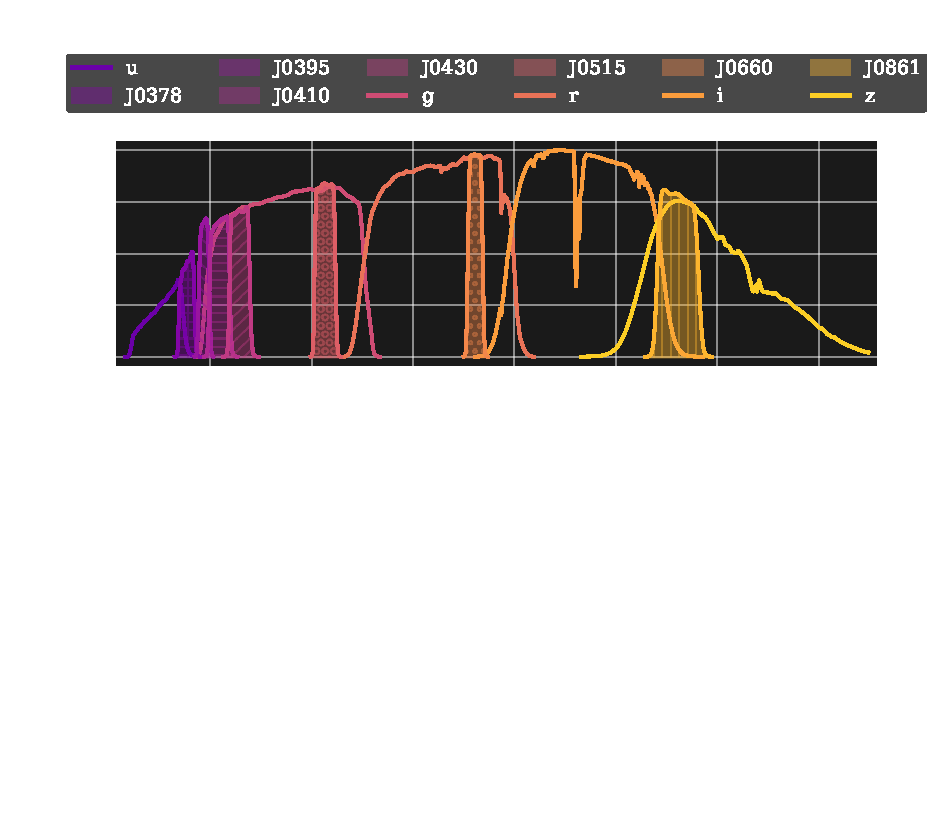
\includegraphics[width=\linewidth]{script/images/transmission_curves.pdf}
    \end{figure}
\end{frame}

\begin{frame}[c]{Dados fotométricos}
    \textbf{Fornax}\\
    \textbf{Run 1}: Faint objects detected near bright galaxies at Fornax distance\\
    \textbf{Run 2}: Better characterizes larger and brighter galaxies
    \begin{columns}[c]
        \begin{column}{0.48\linewidth}
                    \begin{figure}
                        \centering
                        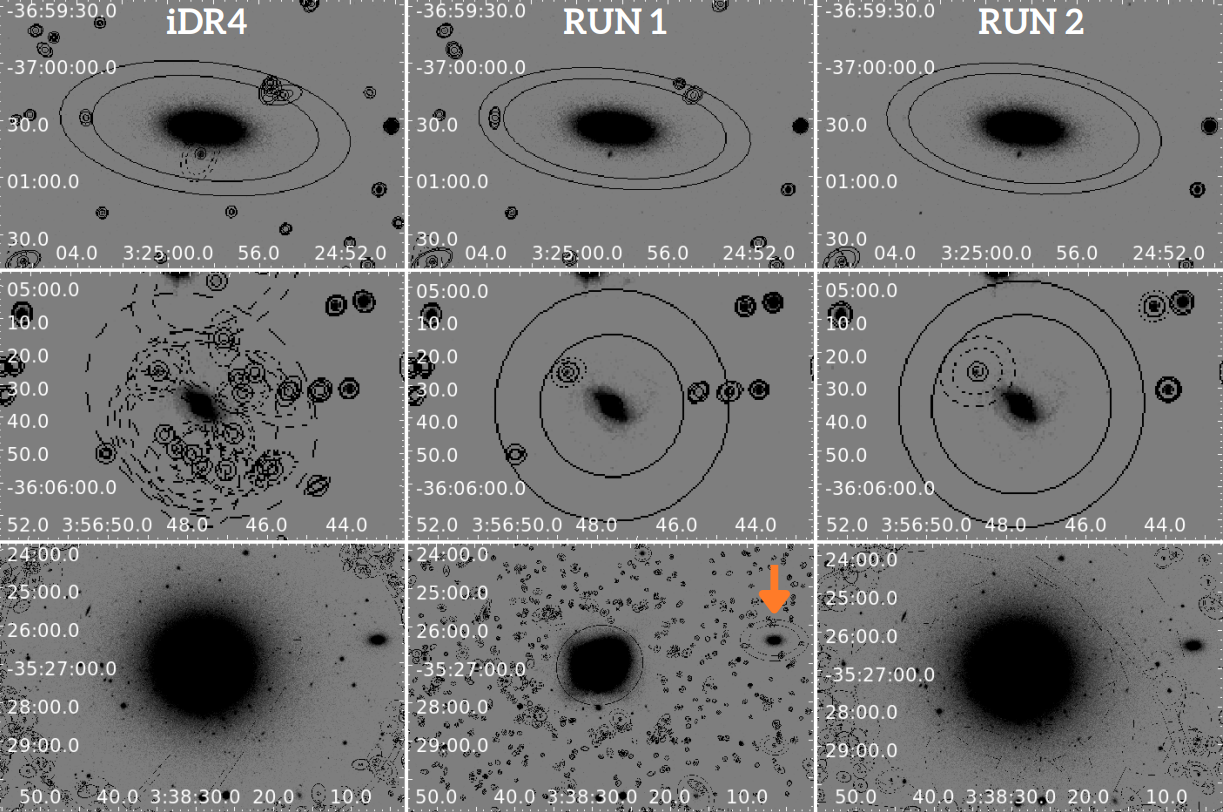
\includegraphics[width=\linewidth]{images/run1.png}
                        \caption{Haack,R.F.(2024)-https://arxiv.org/pdf/2404.10847}
                    \end{figure}
                \end{column}
        \begin{column}{0.48\linewidth}
                    \textbf{Extinction correction}
                    \begin{itemize}
                        \item Galaxy dust affects photometric measurements. Python dustmaps (Green, 2018)
                        \item Calculation of Extinction Coefficients. Python extinction (Barbary 2016)
                    \end{itemize}
                \end{column}
    \end{columns}
\end{frame}

\begin{frame}[c]{Cortes de qualidade na fotometria}
    \begin{splusbox}{Critérios de seleção}
        \begin{itemize}
            \item Magnitudes maiores que 30 foram descartadas (baixa qualidade e erros altos).
            \item Objetos com \texttt{flag0<3} também foram descartados.
            \item Banda \texttt{g\_APER\_6} como referência principal:
            \begin{itemize}
                \item Corte inferior: \texttt{g\_APER\_6} $>$ 13 (evitar saturação).
                \item Corte superior: \texttt{g\_APER\_6} $<$ 21 (minimizar contaminação por aglomerados globulares).
            \end{itemize}
        \end{itemize}
    \end{splusbox}

    \begin{splusbox}{Resultados}
        \begin{itemize}
            \item Total inicial: 2.9 milhões de objetos.
            \item Após cortes: 619.630 objetos restantes.
        \end{itemize}
    \end{splusbox}

\end{frame}

\begin{frame}[c]{Cortes de qualidade na fotometria}
    \begin{figure}
        \centering
            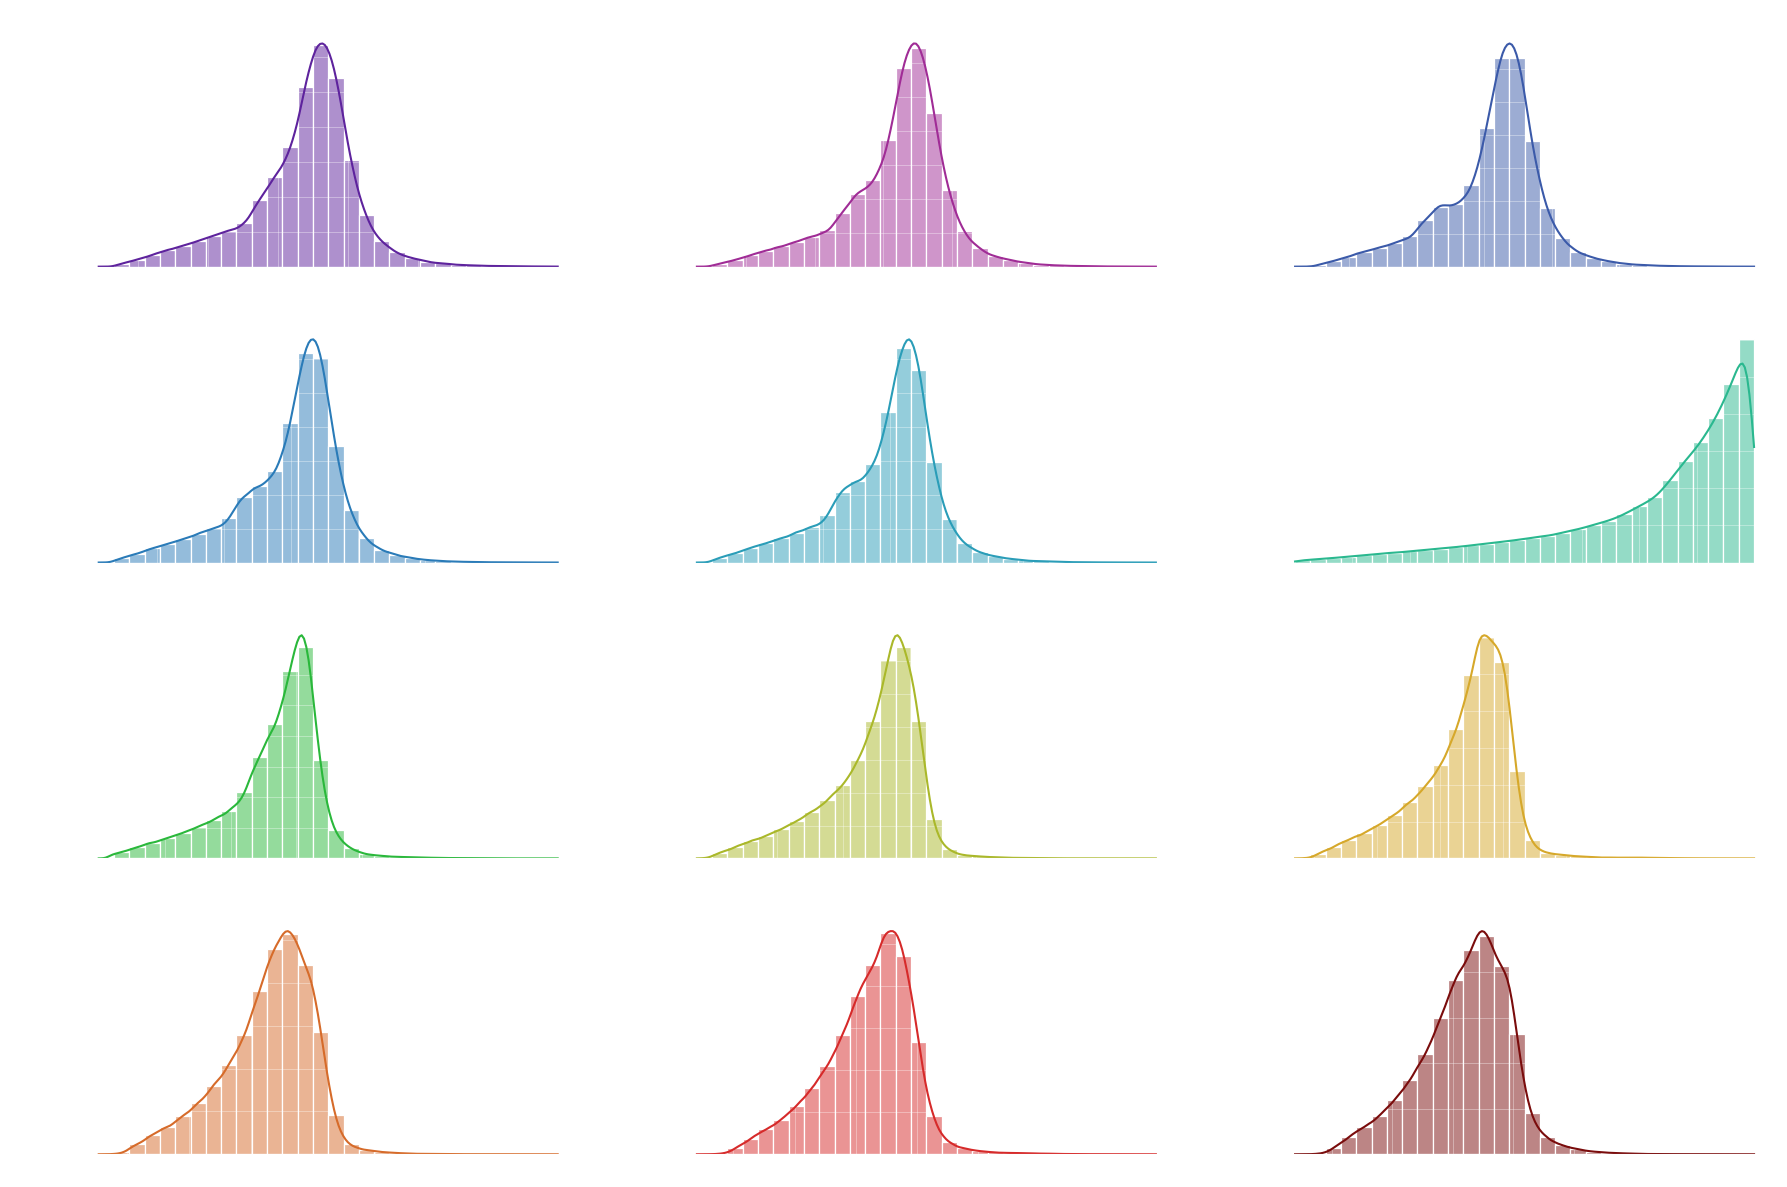
\includegraphics[width=\linewidth, height=6.5cm, keepaspectratio]{images/hist_distri_mags_data.png}
    \end{figure}
\end{frame}

\begin{frame}[c]{Distribuição das UCDs em Fornax}
    \begin{figure}
        \centering
        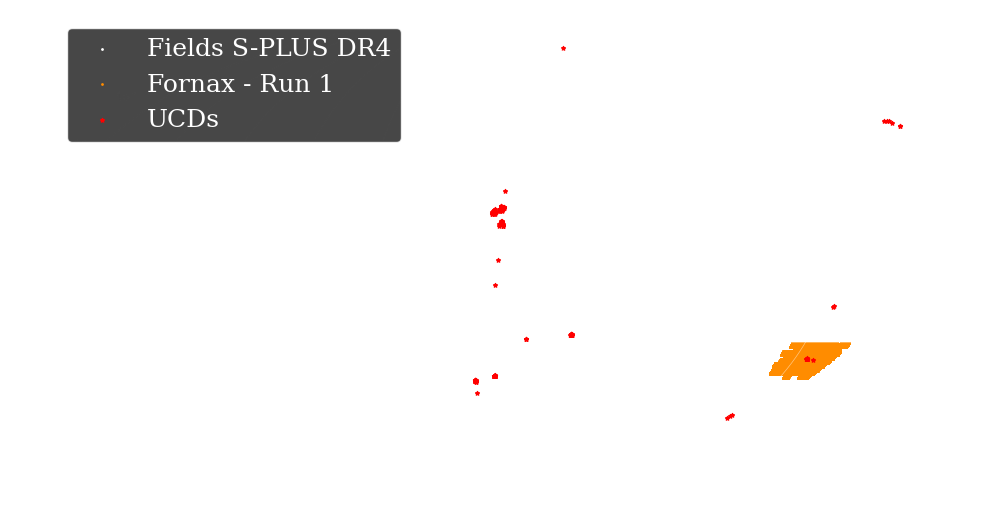
\includegraphics[width=0.8\linewidth, keepaspectratio]{images/ucds_sky.png}
    \end{figure}
\end{frame}

\begin{frame}[c]{Distribuição das UCDs em Fornax}
    \begin{figure}
        \centering
        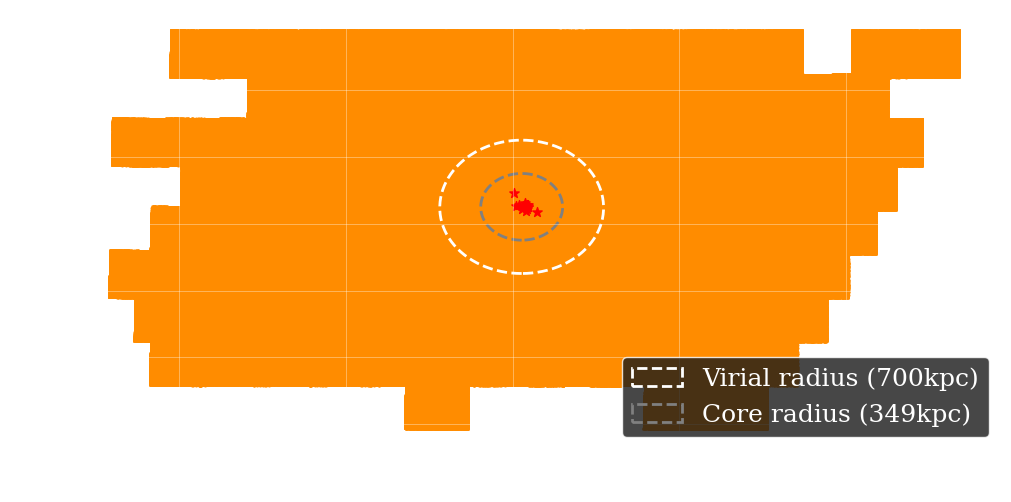
\includegraphics[width=0.8\linewidth, keepaspectratio]{images/zoom_fornax.png}
    \end{figure}
\end{frame}

\begin{frame}[c]{Distribuição das UCDs em Fornax}
    \begin{columns}[c]
        \begin{column}{0.48\textwidth}
            \centering
            \begin{table}[!ht]
                \centering
                \footnotesize
                \begin{tabular}{lc}
                    \toprule
                    \textbf{Parâmetro} & \textbf{Valor} \\ 
                    \midrule
                    Massa ($M_\odot$)$^1$ & $7 \pm 2 \times 10^{13}$ \\ 
                    Raio Virial ($Mpc$)$^1$ & 0.7 \\ 
                    Raio Virial ($graus$)$^1$ & 2 \\ 
                    Raio interno ($Mpc$)$^4$ & 0.349 \\ 
                    Raio interno ($graus$)$^4$ & 1 \\ 
                    $\sigma_v$ ($km \, s^{-1}$)$^3$ & 318 \\ 
                    Módulo de distância ($mag$)$^2$ & 31.51 \\ 
                    \bottomrule
                \end{tabular}
            \end{table}
        \end{column}
        \begin{column}{0.48\textwidth}
            \centering
            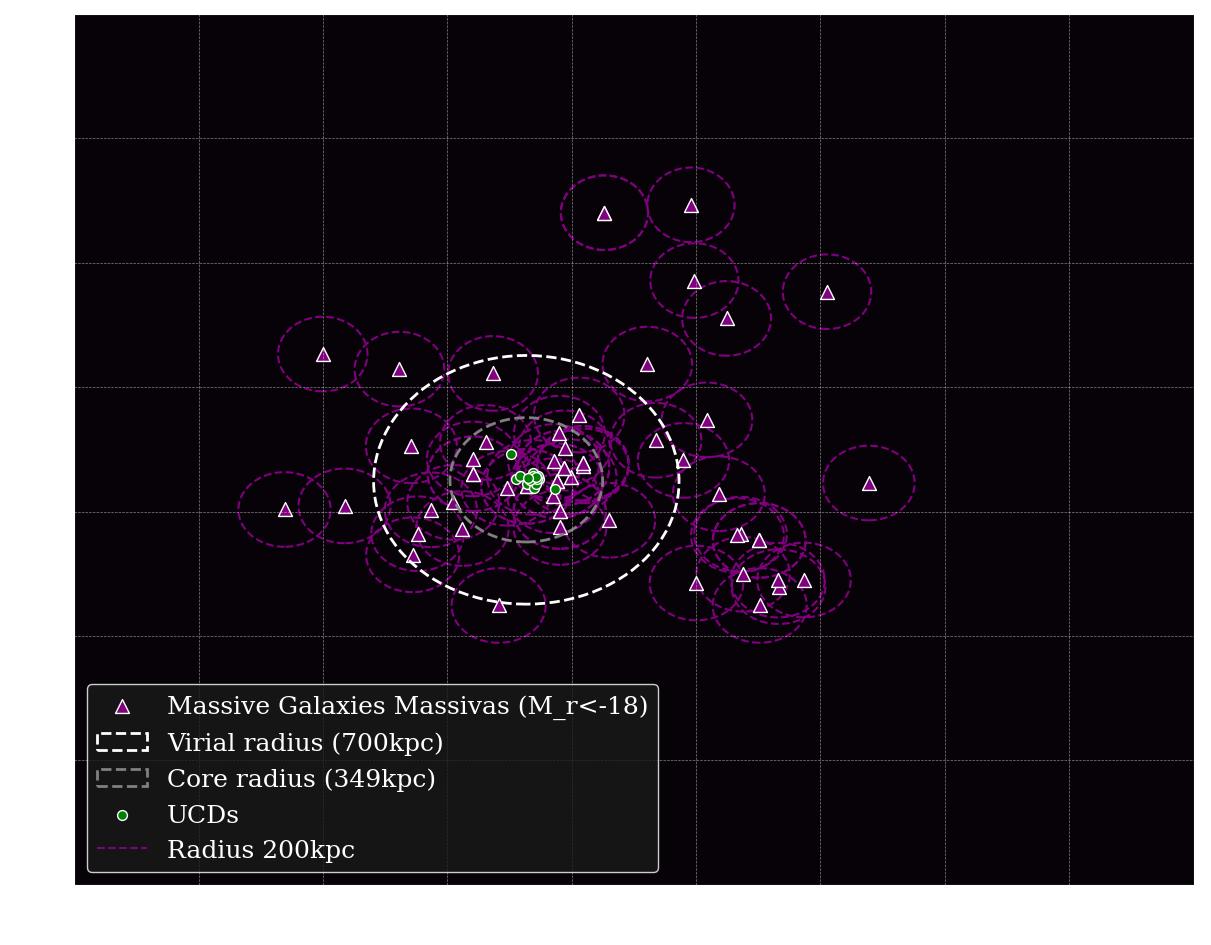
\includegraphics[width=\textwidth, height=0.48\textheight, keepaspectratio]{images/distribuicao_galaxias_massivas.png}
            \vspace{0.5cm}
            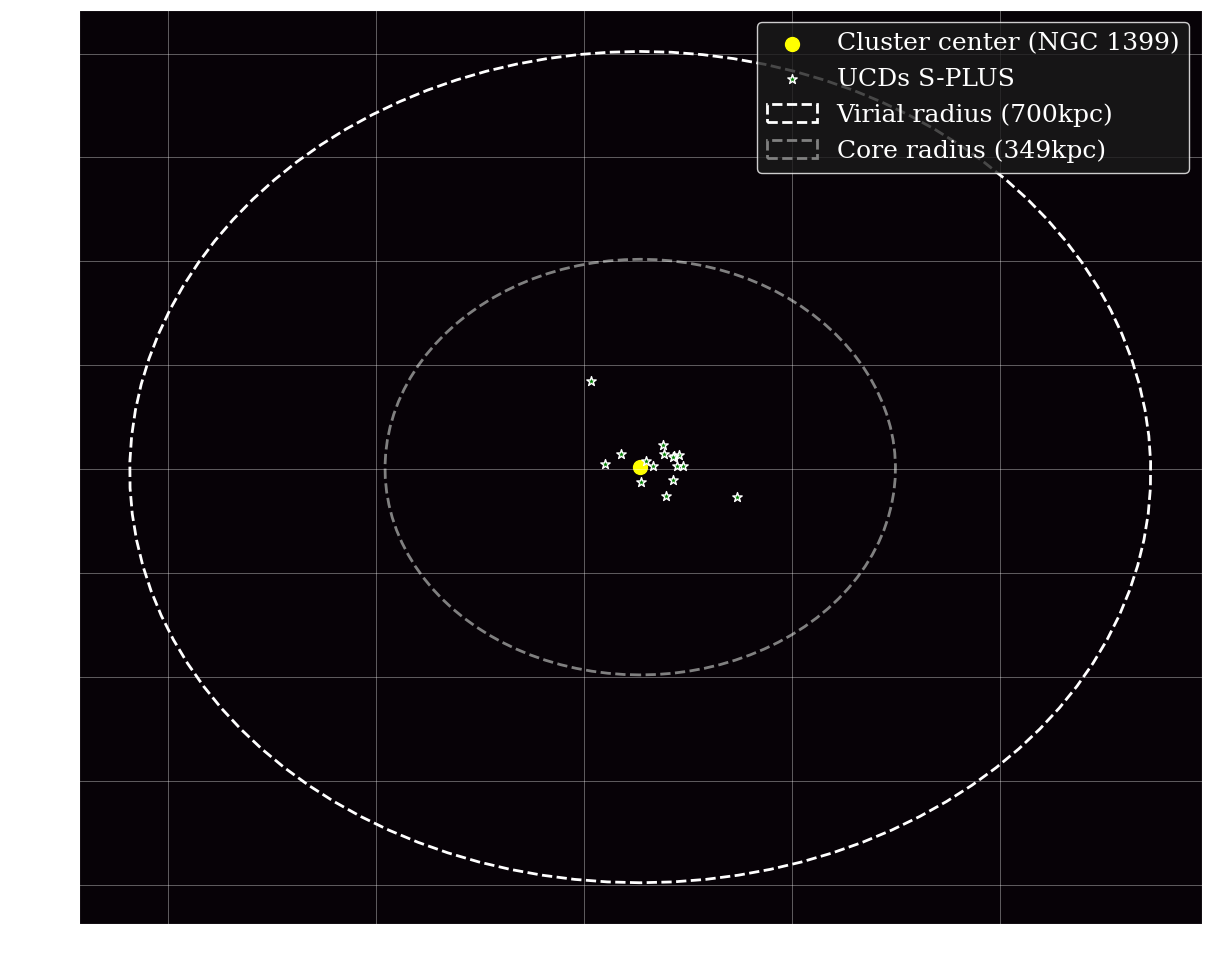
\includegraphics[width=\textwidth, height=0.48\textheight, keepaspectratio]{images/distribuicao_ucds_center.png}
        \end{column}
    \end{columns}
\end{frame}

\begin{frame}[c]{Propriedades das UCDs}
    \vspace{0.2cm}
    \begin{table}[h]
        \centering
        \scriptsize
        \caption{Propriedades das UCDs de Mieske et al.(2008).}
        \begin{tabular}{lccccccc}
        \toprule
        Nome & Massa Total & $M/L_V$ & [Fe/H] & $r_h$ & $\sigma$ \\
        & ($10^6 \, M_\odot$) & & (dex) & (pc) & (km/s)\\
        \midrule
        UCD3, F-19 & $93.6 \pm 14.0$ & $4.69 \pm 0.70$ & -0.4 & 89.7 & 22.8 \\
        UCD1       & $32.1 \pm 3.9$  & $4.99 \pm 0.60$ & -0.7 & 22.4 & 27.1 \\
        F-24       & $24.5 \pm 7.8$  & $3.44 \pm 1.10$ & -0.4 & 29.5 & 21.4 \\
        UCD5       & $18.0 \pm 4.5$  & $3.37 \pm 0.85$ & -1.2 & 31.2 & 18.7 \\
        F-1a       & $16.2 \pm 3.8$  & $2.45 \pm 0.58$ & 0.0  & 23.1 & 18.7 \\
        F-9        & $14.1 \pm 3.6$  & $4.72 \pm 1.20$ & -0.8 & 9.1  & 25.7 \\
        F-5        & $13.7 \pm 2.4$  & $3.16 \pm 0.55$ & -0.3 & 5.0  & 34.5 \\
        F-6        & $12.5 \pm 2.4$  & $5.32 \pm 1.00$ & 0.2  & 7.3  & 27.3 \\
        F-7        & $10.5 \pm 1.4$  & $4.21 \pm 0.57$ & -1.3 & 14.9 & 20.1 \\
        F-12       & $8.3 \pm 2.9$   & $2.36 \pm 0.83$ & -0.4 & 10.3 & 22.9 \\
        F-11       & $5.7 \pm 3.7$   & $1.64 \pm 1.10$ & -0.9 & 3.6  & 26.2 \\
        F-34       & $5.5 \pm 1.3$   & $3.17 \pm 0.74$ & -0.9 & 4.0  & 24.6 \\
        F-22       & $5.3 \pm 1.0$   & $2.13 \pm 0.39$ & -0.4 & 10.0 & 22.8 \\
        F-53       & $3.9 \pm 1.0$   & $2.66 \pm 0.69$ & -0.9 & 4.4  & 19.6 \\
        F-51       & $3.5 \pm 0.9$   & $2.38 \pm 0.62$ & -0.8 & 4.2  & 20.1 \\
        F-59       & $1.3 \pm 0.6$   & $0.94 \pm 0.43$ & -2.1 & 5.7  & 9.8  \\
        \bottomrule
        \end{tabular}
        \label{ucds_fornax_propriedades}
    \end{table}
\end{frame}

\begin{frame}[c]{Propriedades das UCDs}
    \begin{columns}[c]
        \begin{column}{0.48\textwidth}
            \begin{table}[!ht]
                \centering
                \scriptsize
                \begin{tabular}{lccc}
                    \toprule
                    Nome & spec-$z$ & $g$ & zml \\
                    \midrule
                    UCD3 & 0.0053 & 18.47 & 0.03 \\
                    UCD1 & 0.0052 & 19.75 & 0.08 \\
                    F-24 & 0.0063 & 19.66 & 0.04 \\
                    UCD5 & 0.0045 & 19.71 & 0.04 \\
                    F-1a & 0.0042 & 19.66 & -    \\
                    F-9  & 0.0058 & 20.85 & 0.07 \\
                    F-5  & 0.0057 & 20.54 & -    \\
                    F-6  & 0.0037 & 20.48 & -    \\
                    F-7  & 0.0050 & 20.89 & 0.16 \\
                    F-12 & 0.0055 & 20.37 & -    \\
                    F-11 & 0.0059 & 20.40 & -    \\
                    F-34 & 0.0054 & 20.79 & -    \\
                    F-22 & 0.0034 & 20.69 & 0.06 \\
                    F-53 & 0.0020 & 21.57 & -    \\
                    F-51 & 0.0041 & 22.23 & -    \\
                    F-59 & 0.0061 & 21.47 & -    \\
                    \bottomrule
                \end{tabular}
                \label{tab:ucds_know_z_gmag}
            \end{table}
        \end{column}
        \begin{column}{0.48\textwidth}
            \centering
            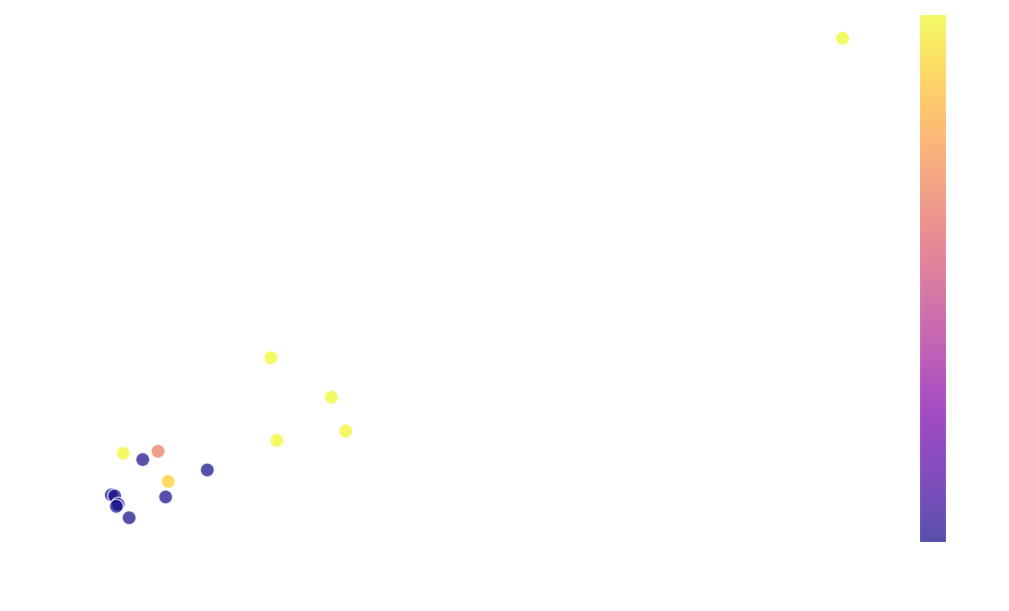
\includegraphics[width=\textwidth, height=0.48\textheight]{images/r_h_M_ucds.png}
            \vspace{0.5cm}
            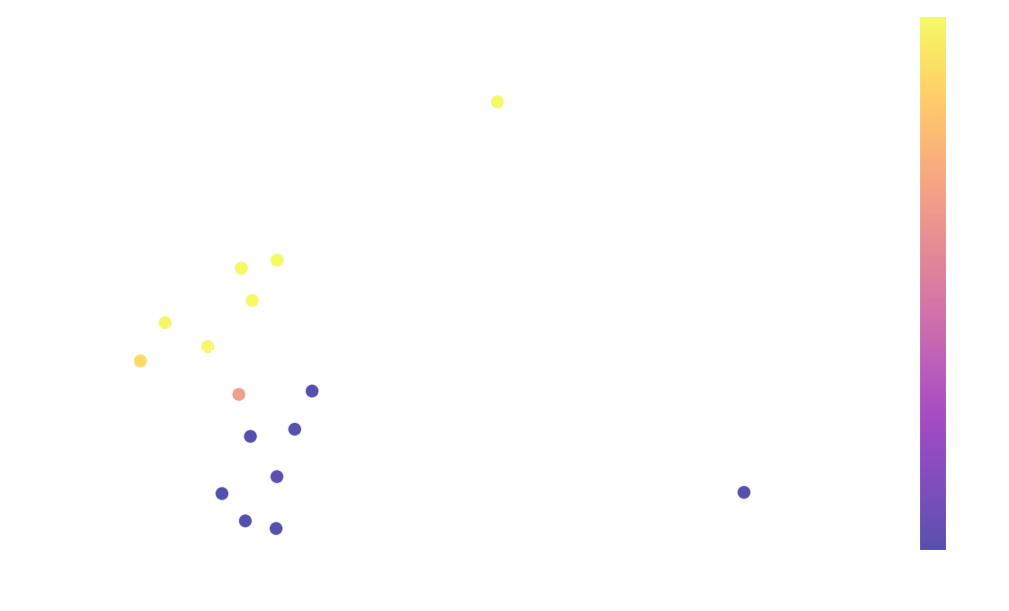
\includegraphics[width=\textwidth, height=0.48\textheight]{images/distribuicao_fwhm_image_r_r_aper6_ucds_fornax.png}
        \end{column}
    \end{columns}
\end{frame}

\section{Aprendizado de máquina}

\begin{frame}[c]{Procura de UCDs com Aprendizado de Máquina}
    \begin{splusbox}{Objetivo}
        \begin{itemize}
            \item Identificar candidatas a galáxias ultra-compactas no aglomerado de Fornax.
            \item Classificar objetos em duas categorias principais:
            \begin{itemize}
                \item Compactos.
                \item Extensos.
            \end{itemize}
            \item Separar objetos com base em suas características morfológicas e fotométricas.
        \end{itemize}
    \end{splusbox}
    \textbf{Identificar dentro do grupo de objetos compactos, aqueles que possuem características fotométricas semelhantes às de galáxias extensas.}
\end{frame}

\begin{frame}[c]{Amostra de Treino e Valores Faltantes}
    \begin{columns}[c]
        \begin{column}{0.48\textwidth}
            \begin{splusbox}{Amostra de Treino}
                \begin{itemize}
                    \item Divisão em classes:
                    \begin{itemize}
                        \item Classe 0: Compactos.
                        \item Classe 1: Extensos.
                    \end{itemize}
                    \item Total de objetos: 545.267.
                    \item Treinamento: 80\% dos dados.
                    \item Teste: 20\% dos dados.
                \end{itemize}
            \end{splusbox}
        \end{column}
        \begin{column}{0.48\textwidth}
            \begin{splusbox}{Valores Faltantes}
                \begin{itemize}
                    \item Imputação com MICE (Método de Imputação Múltipla).
                    \item 27\% dos objetos possuem pelo menos 1 valor faltante.
                    \item Dados faltantes tratados para garantir consistência.
                \end{itemize}
            \end{splusbox}
        \end{column}
    \end{columns}
\end{frame}

\begin{frame}[c]{Distribuição de Valores Faltantes}
    \vspace{0.5cm}
    \begin{figure}
        \centering
        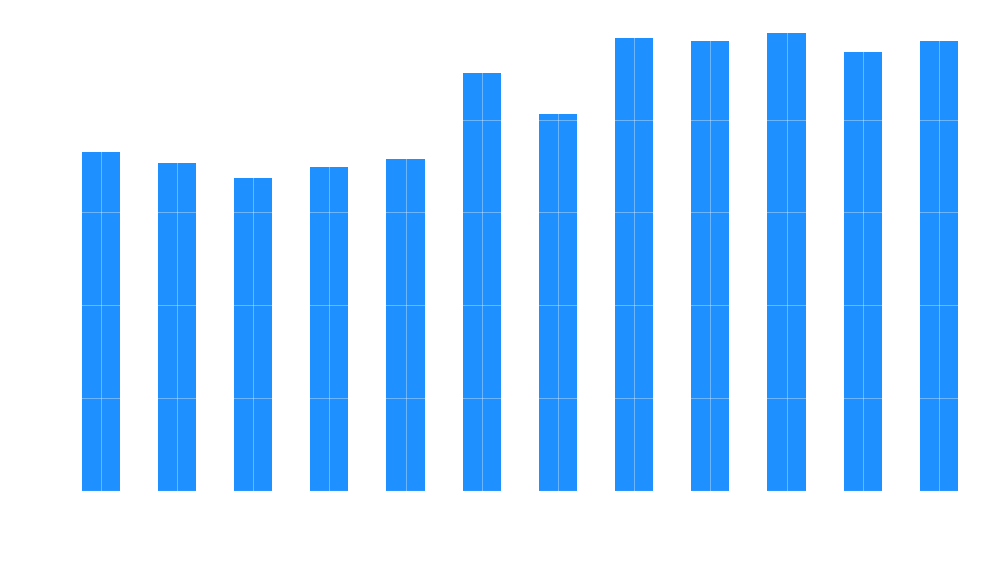
\includegraphics[width=0.8\linewidth, height=6cm, keepaspectratio]{images/missing_values_hist.png}
        \caption{Distribuição de valores faltantes.}
    \end{figure}
\end{frame}

\begin{frame}[c]{Amostra de treino}
    \begin{columns}[c]
        \begin{column}{0.48\textwidth}
            \vspace{0.5cm} % Adiciona espaço acima dos gráficos
            \hspace{0.5cm} % Adiciona espaço horizontal para afastar os gráficos do título
            \begin{figure}
                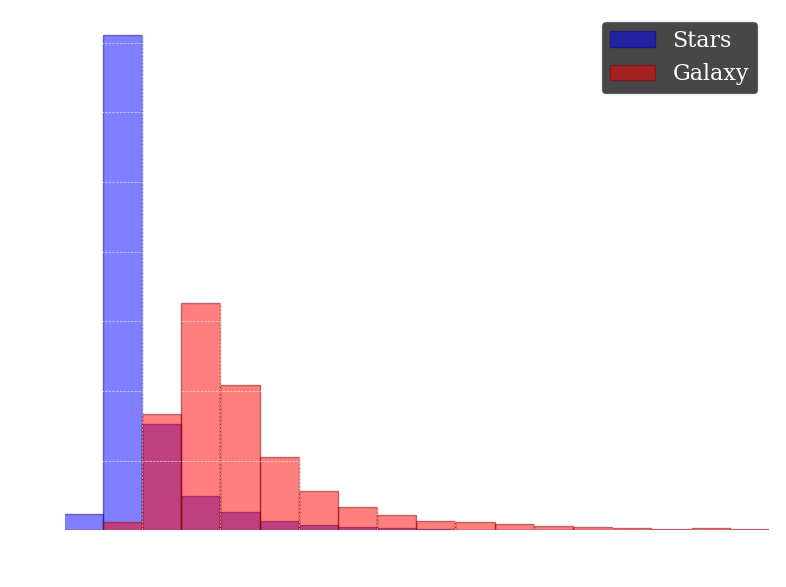
\includegraphics[width=\linewidth, height=0.44\textheight, keepaspectratio]{images/distribution_of_stars_and_galaxies.png}
                \vspace{0.5cm}
                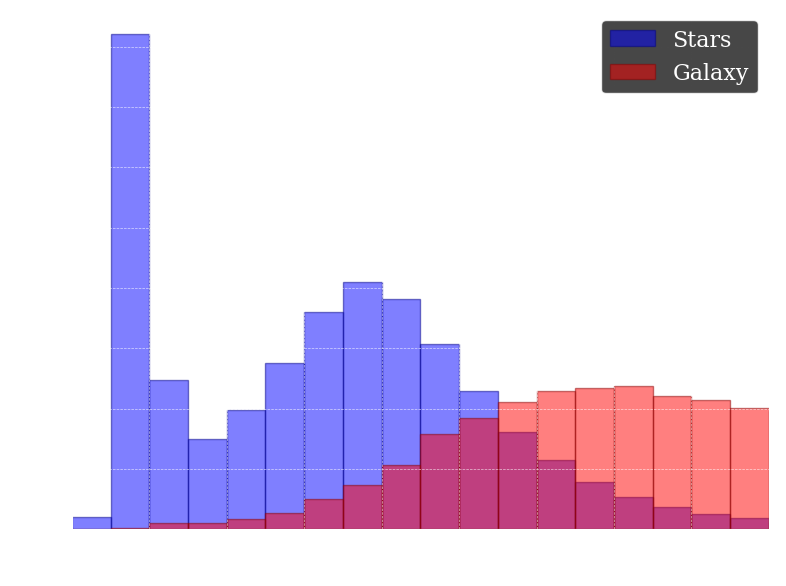
\includegraphics[width=\linewidth, height=0.44\textheight, keepaspectratio]{images/distribution_of_stars_and_galaxies_u.png}
            \end{figure}
        \end{column}
        \begin{column}{0.48\textwidth}
            \footnotesize
            \begin{itemize}
                \item \textbf{Precisão:} $\frac{\text{TP}}{\text{TP} + \text{FP}}$
                \item \textbf{Completeness:} $\frac{\text{TP}}{\text{TP} + \text{FN}}$
                \item \textbf{F1-Score:} $2 \cdot \frac{\text{Precisão} \cdot \text{Completeness}}{\text{Precisão} + \text{Completeness}}$
            \end{itemize}
            \begin{figure}
                \centering
                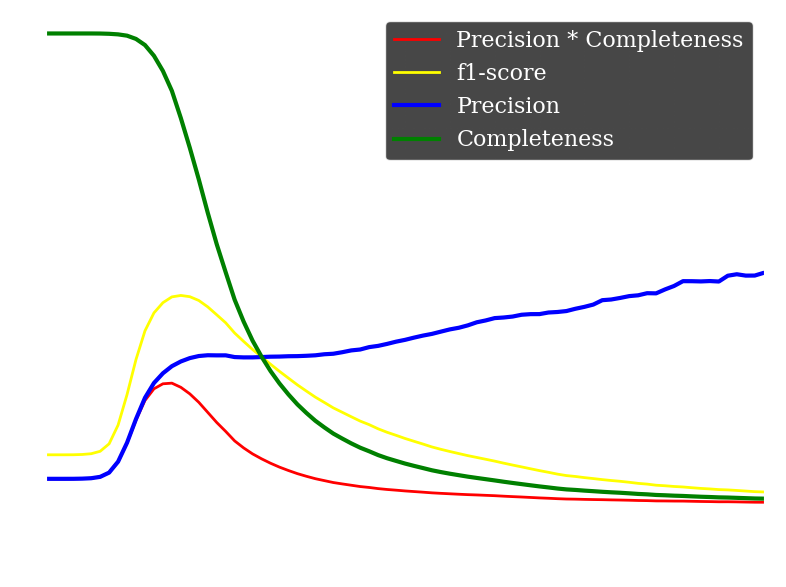
\includegraphics[width=\linewidth, height=0.5\textheight, keepaspectratio]{images/purity_completeness.png}
            \end{figure}
        \end{column}
    \end{columns}
\end{frame}

\begin{frame}[c]{Amostra de treino}
    \begin{columns}[c]
        \begin{column}{0.3\textwidth}
            \begin{splusbox}{\scriptsize Critérios de Classificação}
                \scriptsize
                \begin{itemize}
                    \item Compactos: FWHM $<$ 2 pixels.
                    \item Extensos: FWHM $>$ 2.5 pixels.
                    \item Dados entre 2 e 2.5 pixels não usados no treinamento.
                \end{itemize}
            \end{splusbox}
        \end{column}
        \begin{column}{0.7\textwidth}
            \centering
            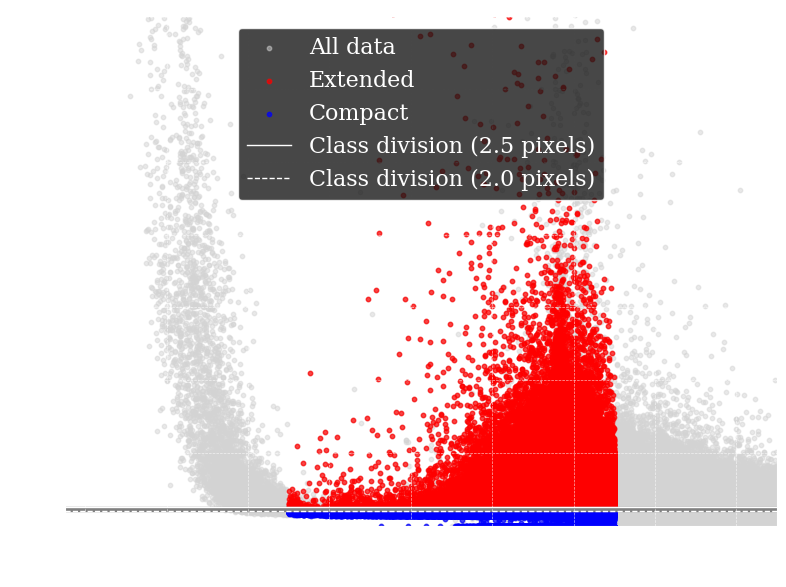
\includegraphics[width=\linewidth]{images/amostra_treino.png}
        \end{column}
    \end{columns}
\end{frame}

\begin{frame}[c]{Amostra de Treino}
    \begin{columns}[c]
        \begin{column}{0.48\textwidth}
            \begin{splusbox}{Divisão da Amostra}
                \begin{itemize}
                    \item Total de objetos: 545.267.
                    \item Treinamento: 80\% (436.213 objetos).
                    \item Teste: 20\% (109.054 objetos).
                    \item Classe 0 (compactos): 242.085 no treino, 60.522 no teste.
                    \item Classe 1 (extensos): 194.128 no treino, 48.532 no teste.
                \end{itemize}
            \end{splusbox}
        \end{column}
        \begin{column}{0.48\textwidth}
            \begin{splusbox}{Parâmetros Utilizados}
                \begin{itemize}
                    \item 12 magnitudes corrigidas pela extinção (\texttt{APER\_6}).
                    \item 66 combinações possíveis de cores.
                    \item Dados entre 2 e 2.5 pixels (FWHM) não usados no treinamento.
                \end{itemize}
            \end{splusbox}
        \end{column}
    \end{columns}
\end{frame}

\begin{frame}[c]{Classificador KNN}
    K-Nearest Neighbors (KNN) 
    \begin{columns}[c]
        \begin{column}{0.48\linewidth}
            \vspace{-1.5cm} % Ajusta o espaço vertical para começar mais acima
            \begin{itemize}
                \item Algoritmo supervisionado que classifica objetos com base nos vizinhos mais próximos.
                \item Simples e eficiente para conjuntos de dados menores.
                \item Utiliza a distância entre objetos no espaço de parâmetros para classificação.
            \end{itemize}
        \end{column}
        \begin{column}{0.48\linewidth}
            \vspace{-1cm} % Ajusta o espaço vertical para começar mais acima
            \begin{figure}
                \centering
                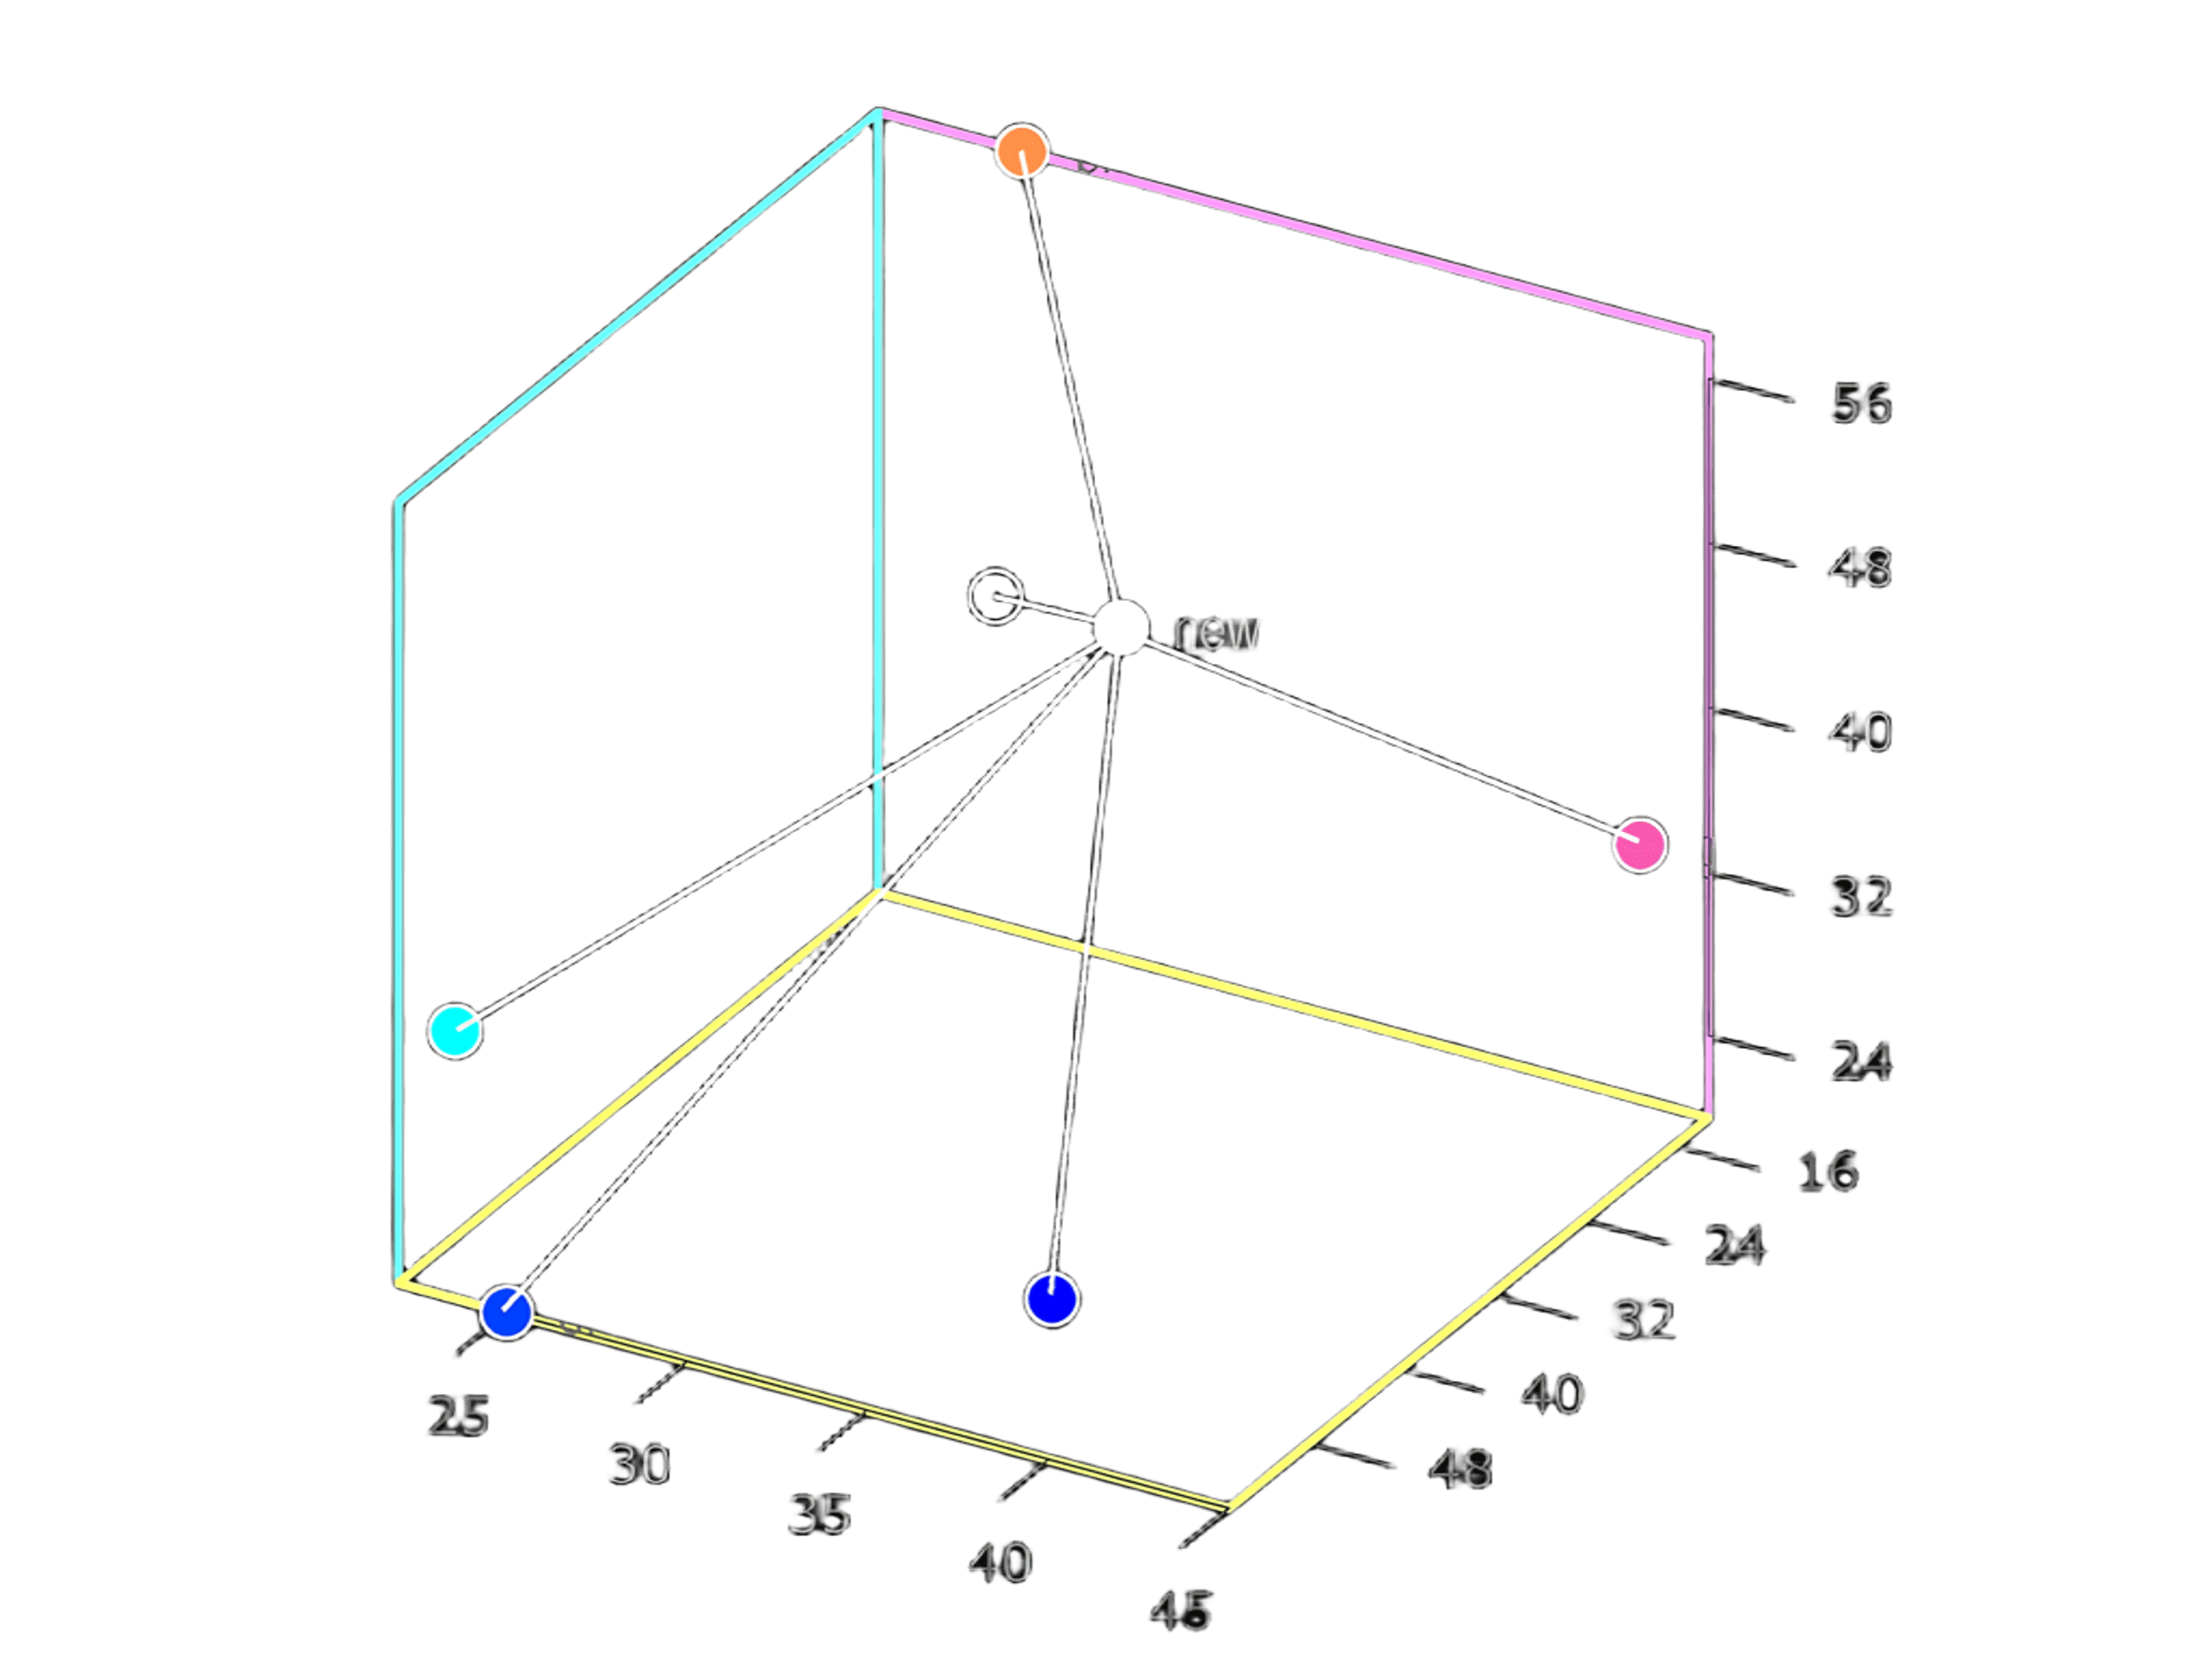
\includegraphics[height=4cm]{images/knn_example1.png}
                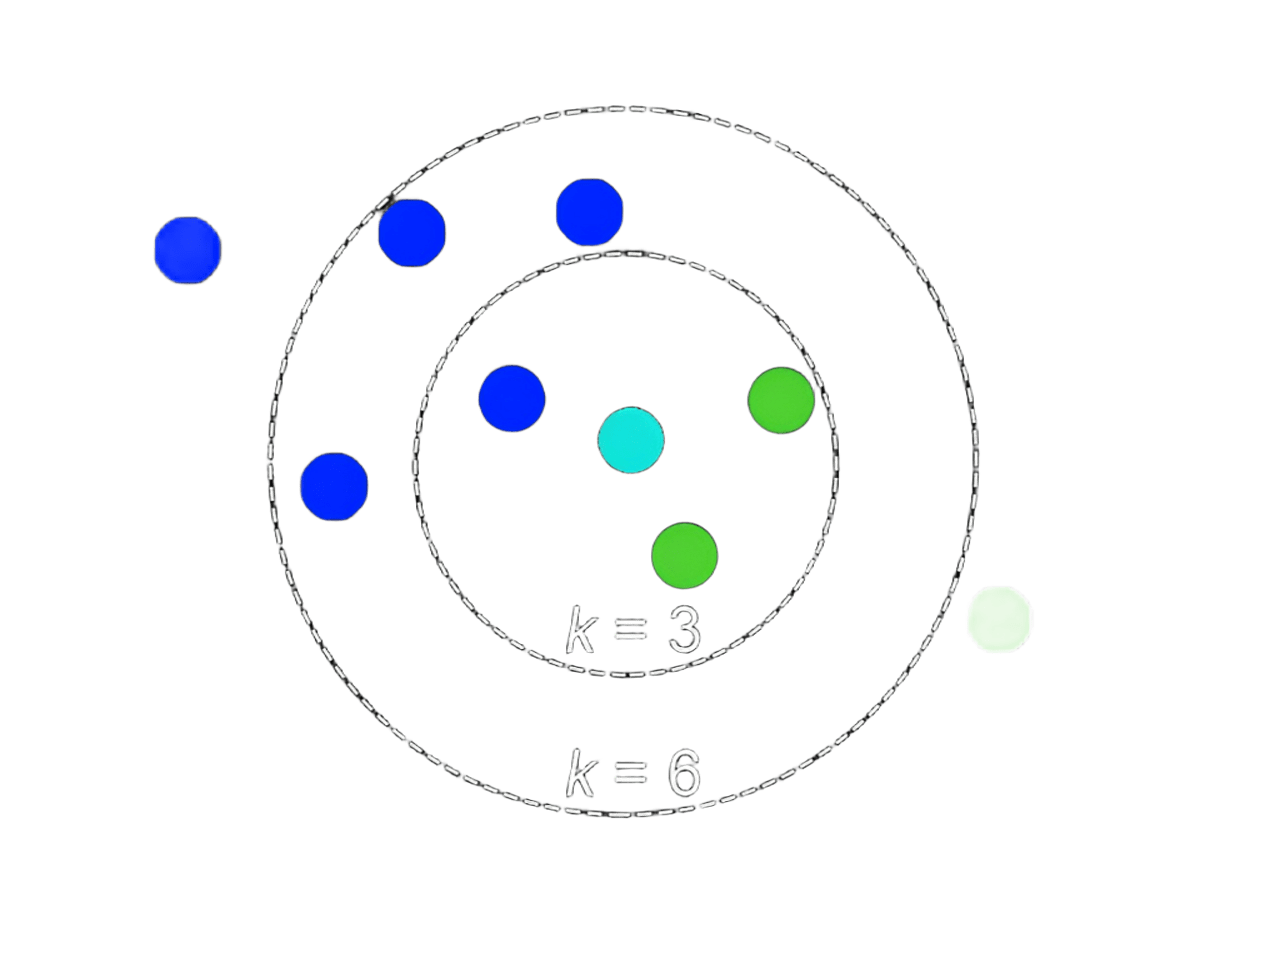
\includegraphics[height=4cm]{images/knn_example2.png}
            \end{figure}
        \end{column}
    \end{columns}
\end{frame}

\begin{frame}[c]{Classificador RF}
    Random Forest (RF)
    \begin{columns}[c]
        \begin{column}{0.48\linewidth}
            \vspace{-1.5cm} % Ajusta o espaço vertical para começar mais acima
            \begin{itemize}
                \item Algoritmo supervisionado baseado em múltiplas árvores de decisão.
                \item Combina os resultados de várias árvores para melhorar a precisão.
                \item Robusto contra overfitting em muitos casos.
                \item Eficiente para conjuntos de dados grandes e com muitas features.
            \end{itemize}
        \end{column}
        \begin{column}{0.48\linewidth}
            \vspace{-1cm} % Ajusta o espaço vertical para começar mais acima
            \begin{figure}
                \centering
                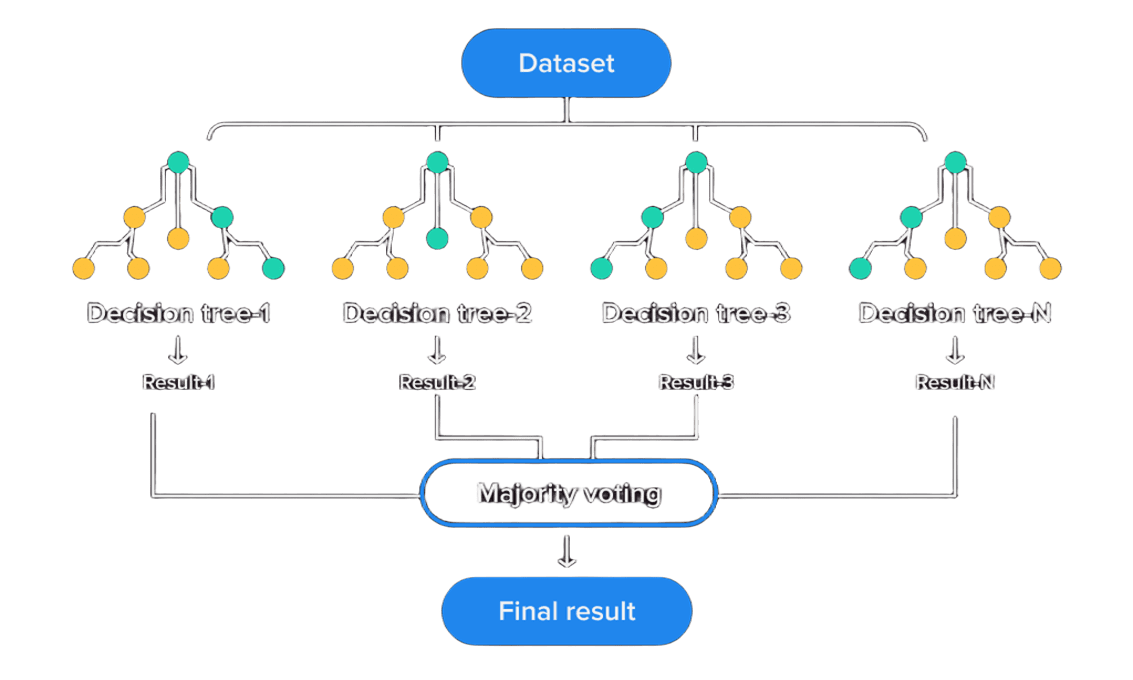
\includegraphics[height=4cm]{images/rf_example1.png}
                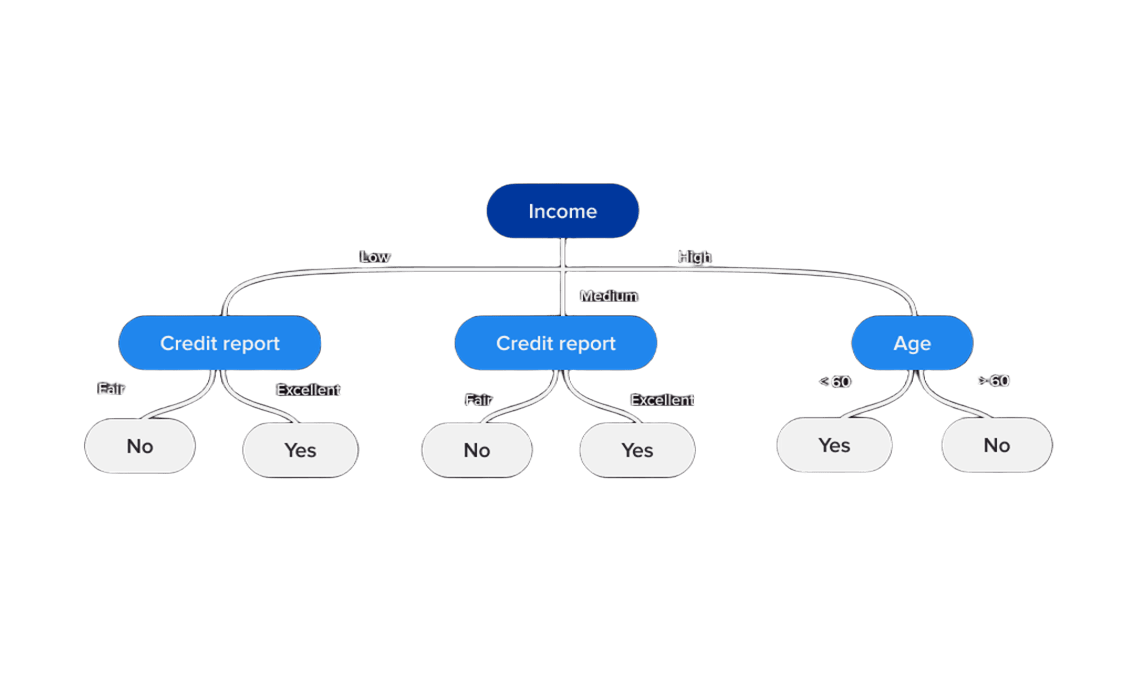
\includegraphics[height=4cm]{images/rf_example2.png}
            \end{figure}
        \end{column}
    \end{columns}
\end{frame}

\begin{frame}[c]{Análise dos Classificadores}
    \begin{columns}[c]
        \begin{column}{0.48\textwidth}
            \vspace{0.4cm}
            \begin{itemize}
                \item \textbf{Acurácia:} 
                \[
                \frac{\text{TP} + \text{TN}}{\text{TP} + \text{TN} + \text{FP} + \text{FN}}
                \]
                \item \textbf{Precisão:} 
                \[
                \frac{\text{TP}}{\text{TP} + \text{FP}}
                \]
                \item \textbf{Completeness:} 
                \[
                \frac{\text{TP}}{\text{TP} + \text{FN}}
                \]
            \end{itemize}
        \end{column}
        \begin{column}{0.48\textwidth}
            \vspace{0.4cm}
            \begin{itemize}
                \item \textbf{F1-Score:} 
                \[
                2 \cdot \frac{\text{Precisão} \cdot \text{Completeness}}{\text{Precisão} + \text{Completeness}}
                \]
                \item \textbf{AUC-ROC:} Mede sensibilidade vs. taxa de falsos positivos.
                \item \textbf{MCC:} 
                \[
                \frac{\text{TP} \cdot \text{TN} - \text{FP} \cdot \text{FN}}{\sqrt{(\text{TP} + \text{FP})(\text{TP} + \text{FN})(\text{TN} + \text{FP})(\text{TN} + \text{FN})}}
                \]
            \end{itemize}
        \end{column}
    \end{columns}
    \vspace{0.5cm}
    \begin{table}[!ht]
        \centering
        \scriptsize
        \begin{tabular}{|c|c|c|}
            \hline
            \textbf{Real} & \textbf{Sim (Detectada)} & \textbf{Não (Detectada)} \\ \hline
            Sim           & Verdadeiro Positivo (TP) & Falso Negativo (FN)      \\ \hline
            Não           & Falso Positivo (FP)      & Verdadeiro Negativo (TN) \\ \hline
        \end{tabular}
        \caption{Matriz de Confusão.}
    \end{table}
\end{frame}

\begin{frame}[c]{Análise dos Classificadores}
    \begin{columns}[c]
        \begin{column}{0.48\textwidth}
            \vspace{-0.8cm} % Ajusta o espaço vertical para começar mais acima
            \scriptsize
            \begin{table}[!ht]
                \centering
                \caption{Classificação binária - Métricas modelo KNN}
                \begin{tabular}{lccc}
                    \toprule
                    Classe & Precisão & Completeza & F1-Score \\
                    \midrule
                    0 & 0.92 & 0.88 & 0.90 \\
                    1 & 0.86 & 0.91 & 0.88 \\
                    \midrule
                    \multicolumn{3}{l}{AUC-ROC} & 0.95 \\
                    \multicolumn{3}{l}{Coeficiente de Correlação de Matthews (MCC)} & 0.78 \\
                    \bottomrule
                \end{tabular}
            \end{table}
            % \vspace{0.2cm}
            \begin{table}[!ht]
                \centering
                \caption{Classificação binária - Métricas modelo RF}
                \begin{tabular}{lccc}
                    \toprule
                    Classe & Precisão & Completeza & F1-Score \\
                    \midrule
                    0 & 0.95 & 0.90 & 0.92 \\
                    1 & 0.89 & 0.94 & 0.91 \\
                    \midrule
                    \multicolumn{3}{l}{AUC-ROC} & 0.97 \\
                    \multicolumn{3}{l}{Coeficiente de Correlação de Matthews (MCC)} & 0.84 \\
                    \bottomrule
                \end{tabular}
            \end{table}
        \end{column}
        % Coluna da direita com as imagens
        \begin{column}{0.48\textwidth}
            \centering
            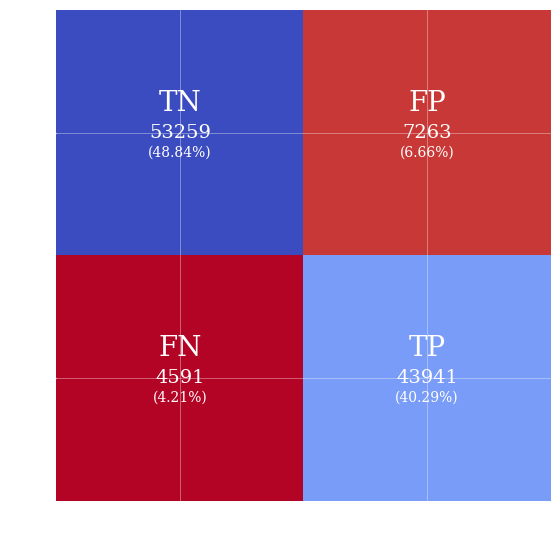
\includegraphics[width=\linewidth, height=4.2cm, keepaspectratio]{images/confusion_matrix_knn.png}
            \vspace{0.5cm}
            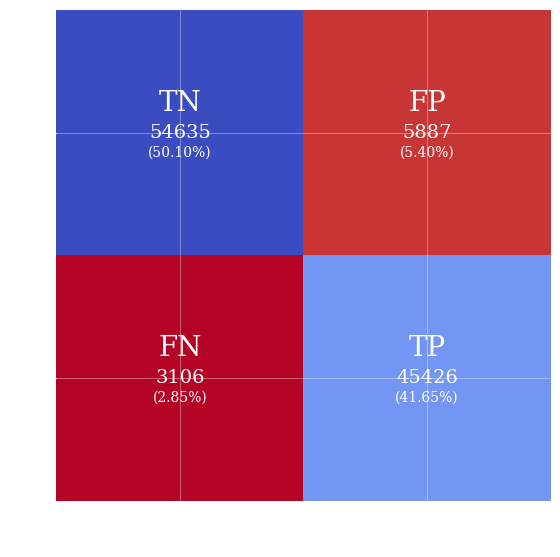
\includegraphics[width=\linewidth, height=4.2cm, keepaspectratio]{images/confusion_matrix_rf.png}
        \end{column}
    \end{columns}
\end{frame}

\begin{frame}[c]{Análise dos Classificadores}
    \begin{columns}[c]
        \begin{column}{0.42\textwidth} % Aumenta a largura da coluna da primeira imagem
            \centering
            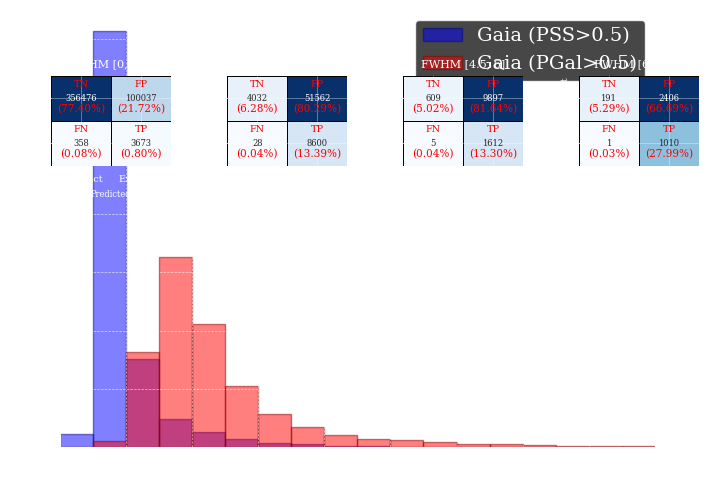
\includegraphics[width=\linewidth, height=0.5\textheight, keepaspectratio]{images/distribution_of_stars_and_galaxies_with_cm.png}
        \end{column}
        \begin{column}{0.4\textwidth} % Aumenta a largura da coluna da segunda imagem
            % \centering
            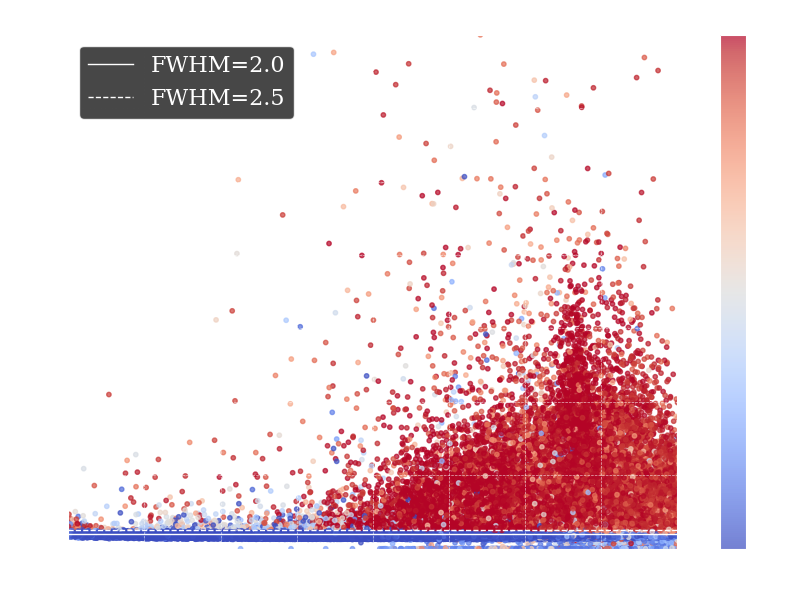
\includegraphics[width=\linewidth, height=0.5\textheight, keepaspectratio]{images/predic_colored.png}
        \end{column}
        \begin{column}{0.2\textwidth} % Reduz a largura da coluna da tabela
            \tiny
            \begin{table}[H]
                \centering
                \begin{tabular}{lc}
                    \toprule
                    Nome & RF Predição \\
                    \midrule
                    UCD3 & 0.36 \\
                    UCD1 & 0.98 \\
                    F-24 & 0.99 \\
                    UCD5 & 0.38 \\
                    F-1a & 0.11 \\
                    F-9 & 0.87 \\
                    F-5 & 0.53 \\
                    F-6 & 0.89 \\
                    F-7 & 0.70 \\
                    F-12 & 0.73 \\
                    F-11 & 0.97 \\
                    F-34 & 0.98 \\
                    F-22 & 0.93 \\
                    F-53 & 0.96 \\
                    F-51 & 0.96 \\
                    F-59 & 0.92 \\
                    \bottomrule
                \end{tabular}
            \end{table}
        \end{column}
    \end{columns}
    % \vspace{0.1cm}
        \begin{splusbox}{\scriptsize}
            \scriptsize
            \begin{itemize}
                \item \textbf{Total de objetos:} 1.803.561.
                \item \textbf{Extensos:} 1.411.803 (78,28\%). Deles 311.846 (17,29\%) com $FWHM < 2.5$ pixels.
            \end{itemize}
        \end{splusbox}
\end{frame}

\begin{frame}[c]{Redshifts Fotométricos}
    Redshifts fotométricos são estimativas baseadas em fotometria multibanda. 
    \begin{equation}
        v_\text{res} = c \cdot z = H_0 \cdot D,
    \end{equation}

    \begin{columns}
        \begin{column}{0.46\linewidth}
            \centering
            \footnotesize
            \textbf{Modelo Treinado}
            \begin{itemize}
                \item Photo-z de \textit{Lima et al. 2022}. 
                \item De 29000926, \textbf{290637} sem estimativa.
                \item $0.002 \leq z \leq 0.5$ ; $15 \leq r_{APER\_6} \leq 21$.
                \item Amostra final: 12.296 objetos.
                \item Treinamento com 66 cores (\texttt{APER\_6}).
                \item Divisão da amostra: 80\% treino, 20\% teste.
                \item Regressão com Random Forest (RF).
            \end{itemize}
        \end{column}
        \begin{column}{0.46\linewidth}
            \begin{figure}
                \centering
                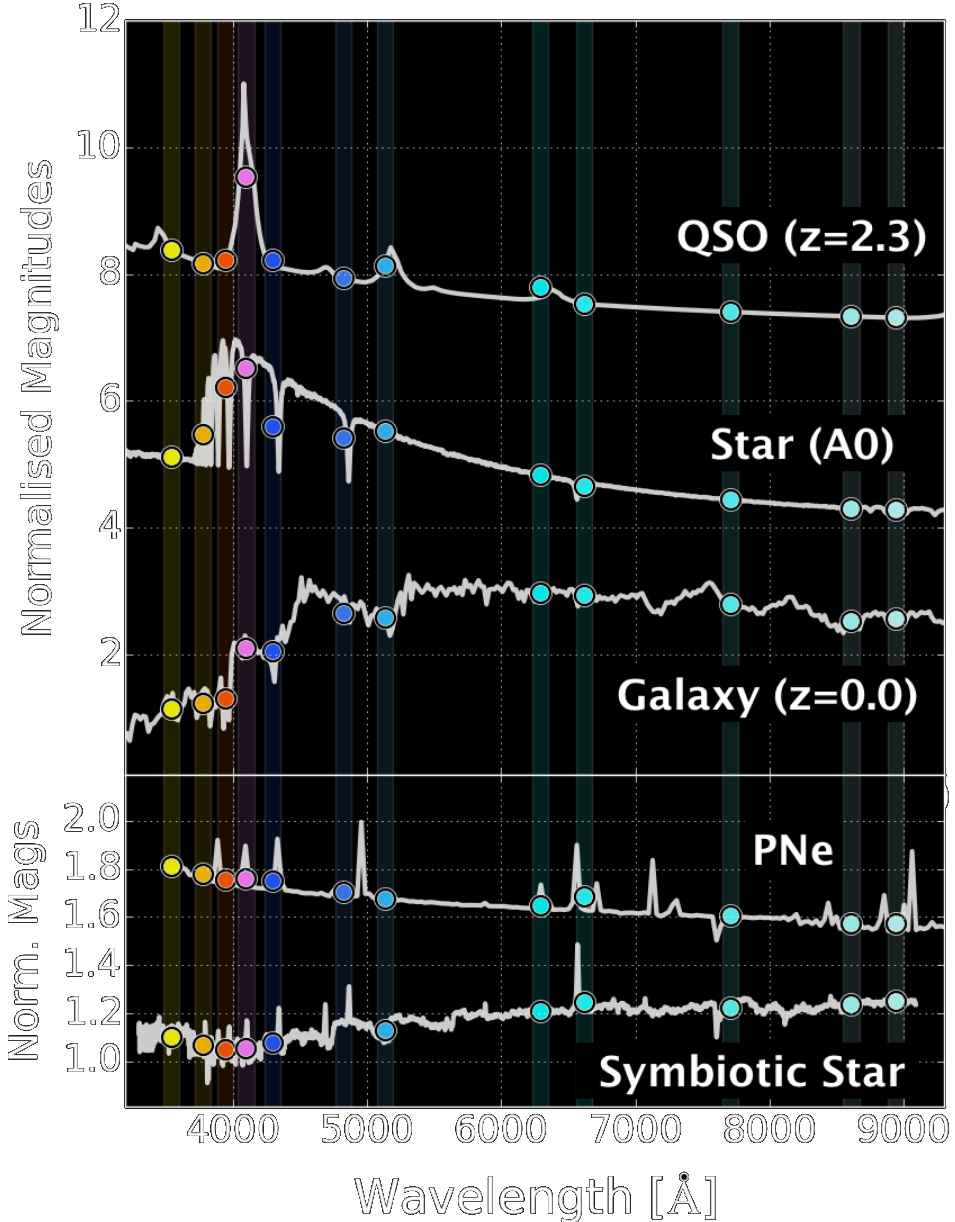
\includegraphics[height=5cm]{script/images/splus_spectra_sed.png}
                \caption{Adaptado de Mendes de Oliveira et al. (2019).}
            \end{figure}
        \end{column}
    \end{columns}
\end{frame}

\begin{frame}[c]{Redshifts Fotométricos}
    \vspace{0.5cm}
    \begin{figure}
        \centering
        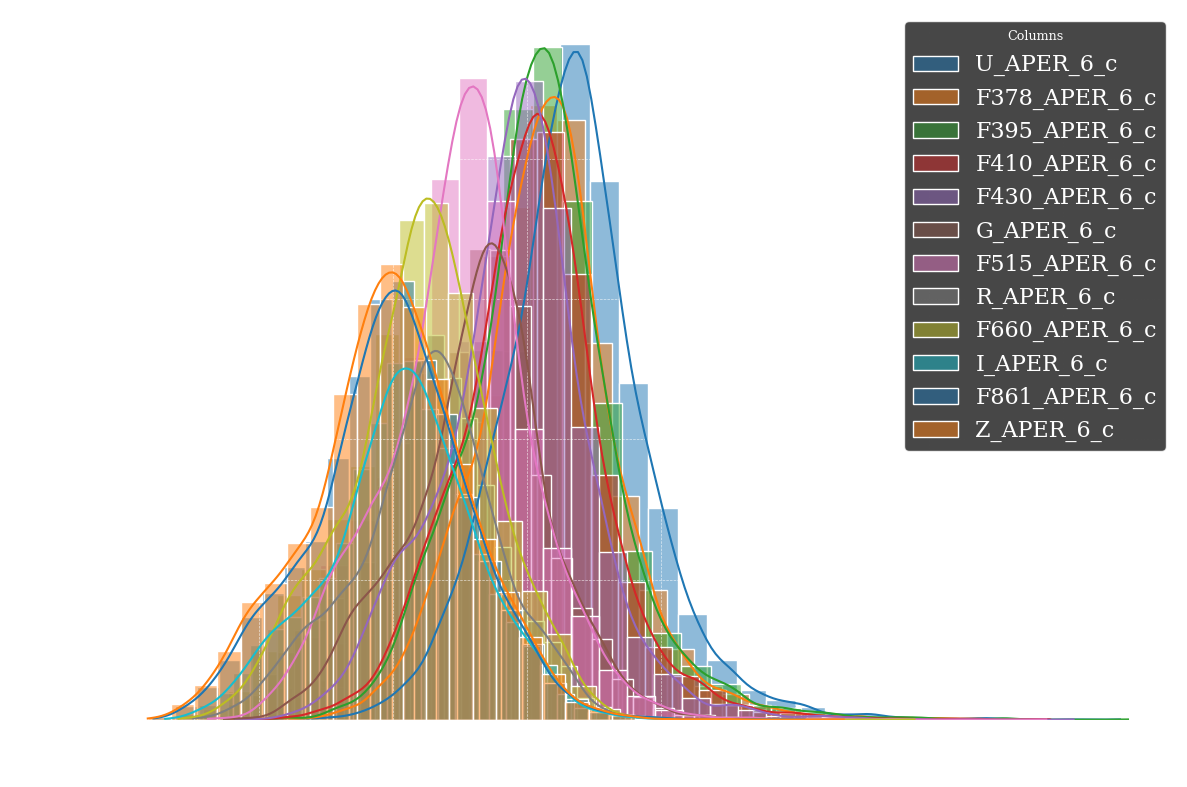
\includegraphics[width=1.\linewidth, height=6cm, keepaspectratio]{images/overlaid_histogram_mags_aper_6_c.png}
        \caption{Distribuição magnitudes na amostra de treino \textit{photo\_z}.}
    \end{figure}
\end{frame}

\begin{frame}[c]{Redshifts Fotométricos}
    \begin{columns}[c]
        \begin{column}{0.32\linewidth}
            \begin{figure}
                \centering
                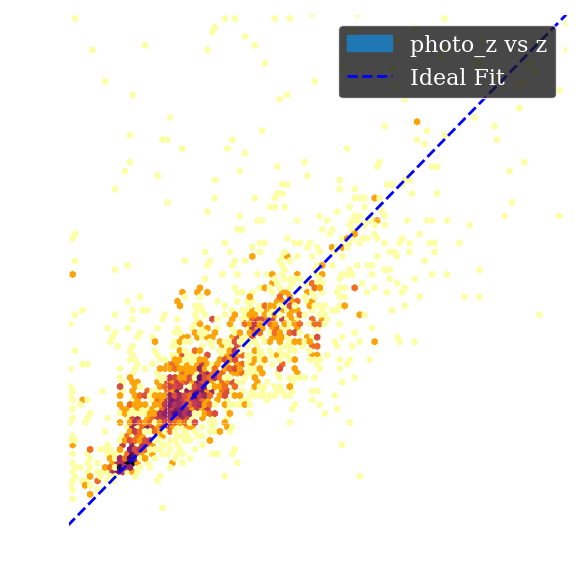
\includegraphics[width=\linewidth]{images/photo_z_test.png}
            \end{figure}
        \end{column}
        \begin{column}{0.32\linewidth}
            \begin{figure}
                \centering
                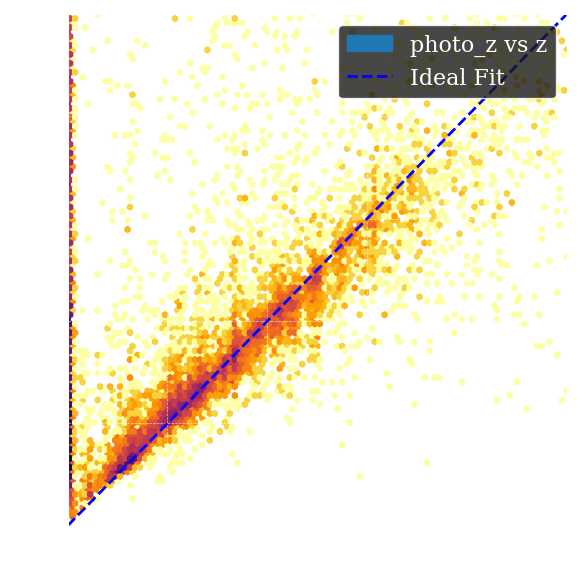
\includegraphics[width=\linewidth]{images/photo_z.png}
            \end{figure}
        \end{column}
        \begin{column}{0.32\linewidth}
            \begin{figure}
                \centering
                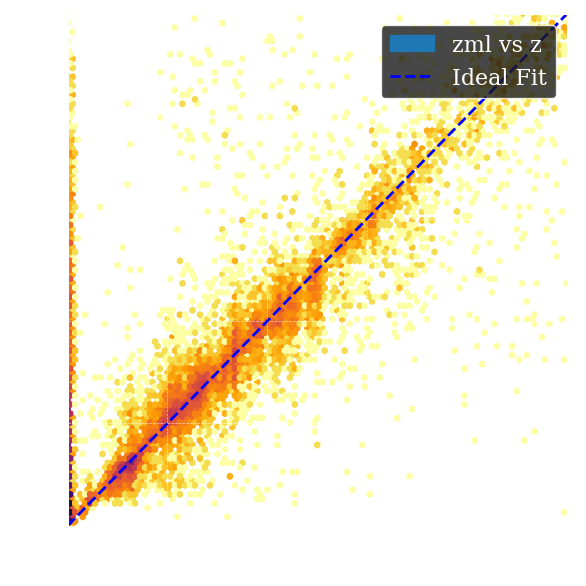
\includegraphics[width=\linewidth]{images/zml.png}
            \end{figure}
        \end{column}
    \end{columns}
    % \vspace{0.5cm}
    \begin{splusbox}{}
        \tiny
        \begin{itemize}
            \item \textbf{EQR =} 0.05
            \item \textbf{$R^2$ =} 0.6
            \item \textbf{$\sigma_{NMAD}$ =} 0.03
        \end{itemize}
    \end{splusbox}
\end{frame}

\begin{frame}[c]{Redshifts Fotométricos}
    \begin{columns}[c]
        \begin{column}{0.7\linewidth}
            \begin{figure}
                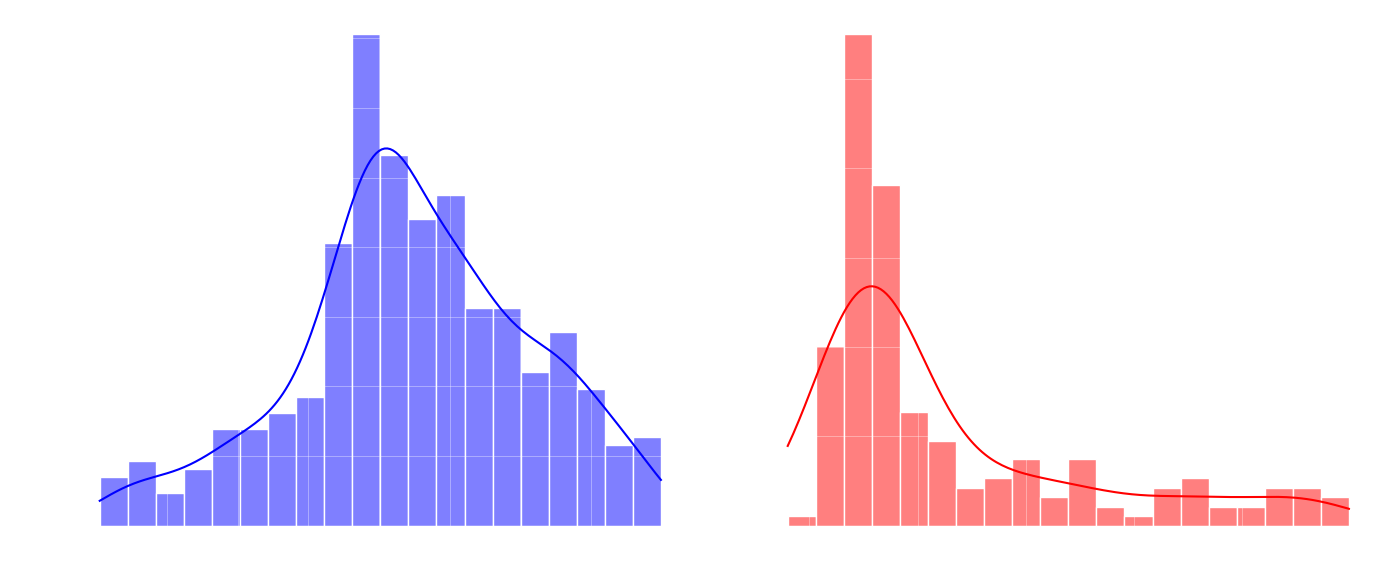
\includegraphics[width=\linewidth]{images/z_zml_distribution.png}
            \end{figure}
        \end{column}
        \begin{column}{0.3\linewidth}
            \begin{table}[!ht]
                \centering
                \scriptsize
                \begin{tabular}{lccc}
                    \toprule
                    Nome & \textit{$z_{phot}$} & \textit{zml} & \textit{$z_{spec}$}\\
                    \midrule
                    UCD3 & 0.07 & 0.03 & 0.0053\\
                    UCD1 & 0.09 & 0.08 & 0.0052\\
                    F-24 & 0.08 & 0.04 & 0.0062\\
                    UCD5 & 0.03 & 0.04 & 0.0045\\
                    F-1a & 0.21 & -- & 0.0042\\
                    F-9 & 0.09 & 0.07 & 0.0058\\
                    F-5 & 0.06 & -- & 0.0057\\
                    F-6 & 0.10 & -- & 0.0037\\
                    F-7 & 0.19 & 0.16 & 0.0050\\
                    F-12 & 0.07 & -- & 0.0055\\
                    F-11 & 0.10 & -- & 0.0059\\
                    F-34 & 0.07 & -- & 0.0054\\ 
                    F-22 & 0.09 & 0.06 & 0.0034\\
                    F-53 & 0.31 & -- & 0.0020\\
                    F-51 & 0.10 & -- & 0.0041\\
                    F-59 & 0.06 & -- & 0.0060\\
                    \midrule
                \end{tabular}
            \end{table}
        \end{column}
    \end{columns}
\end{frame}

\begin{frame}[c]{Seleção das candidatas}

\begin{columns}[c]
    \begin{column}{0.48\textwidth}
        \vspace{0.2cm}
        \begin{splusbox}{\tiny Seleções aplicadas (Total 1.803.561 objetos)}
            \tiny
            \begin{itemize}
                \item Corte de magnitude: $18 \leq r_\text{APER\_6} < 21$.
                \item Extended Probability $> 0.9$.
                \item Corte de FWHM: $FWHM_r \leq 2.5$ pixels.
                \item \textit{photo\_z} $\leq 0.05$.
            \end{itemize}
        \end{splusbox}
    \end{column}
    \begin{column}{0.48\textwidth}
        \vspace{0.2cm}    
        \begin{table}[!ht]
            \centering
            \tiny
            \begin{tabular}{l l r r}
                \hline
                \multicolumn{4}{c}{$y = ax + b$}\\
                \hline
                y & x & a & b\\
                \hline
                FR (90\%-20\%) & r & -4.5 & 97 \\
                FR (90\%-20\%) & r & -0.8 & 17 \\
                FR (90\%-70\%) & FR 90\% & 0.7 & -0.8 \\
                FR (90\%-70\%) & FR 90\% & 0.3 & -0.45 \\
                FR (70\%-20\%) & FR (90\%-70\%) & 1.6 & 1 \\
                FR (70\%-20\%) & FR (90\%-70\%) & 0.4 & 0.05 \\
                \hline
            \end{tabular}
            \label{cortes_flux_radius}
        \end{table}
    \end{column}
\end{columns}
\begin{columns}[c]
    \begin{column}{0.32\linewidth}
        \begin{figure}
            \centering
            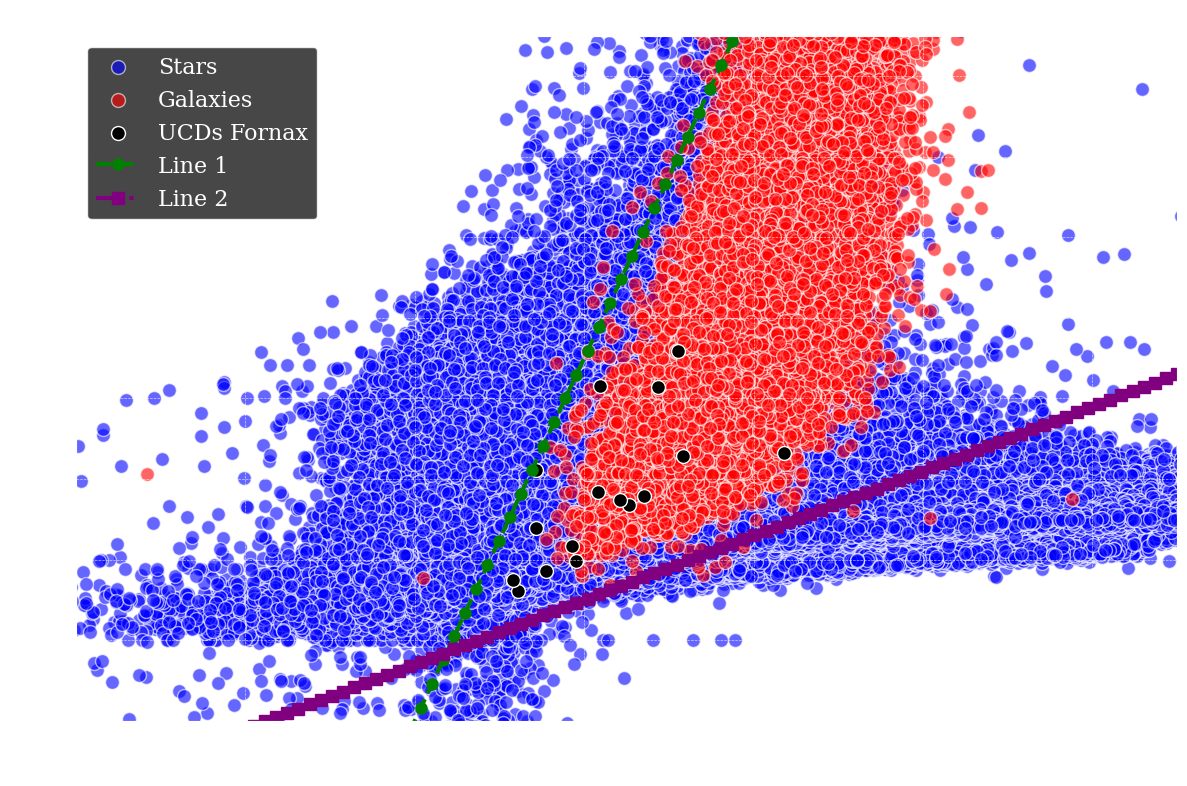
\includegraphics[width=\linewidth]{images/f_90_20_R_APER_6.png}
        \end{figure}
    \end{column}
    \begin{column}{0.32\linewidth}
        \begin{figure}
            \centering
            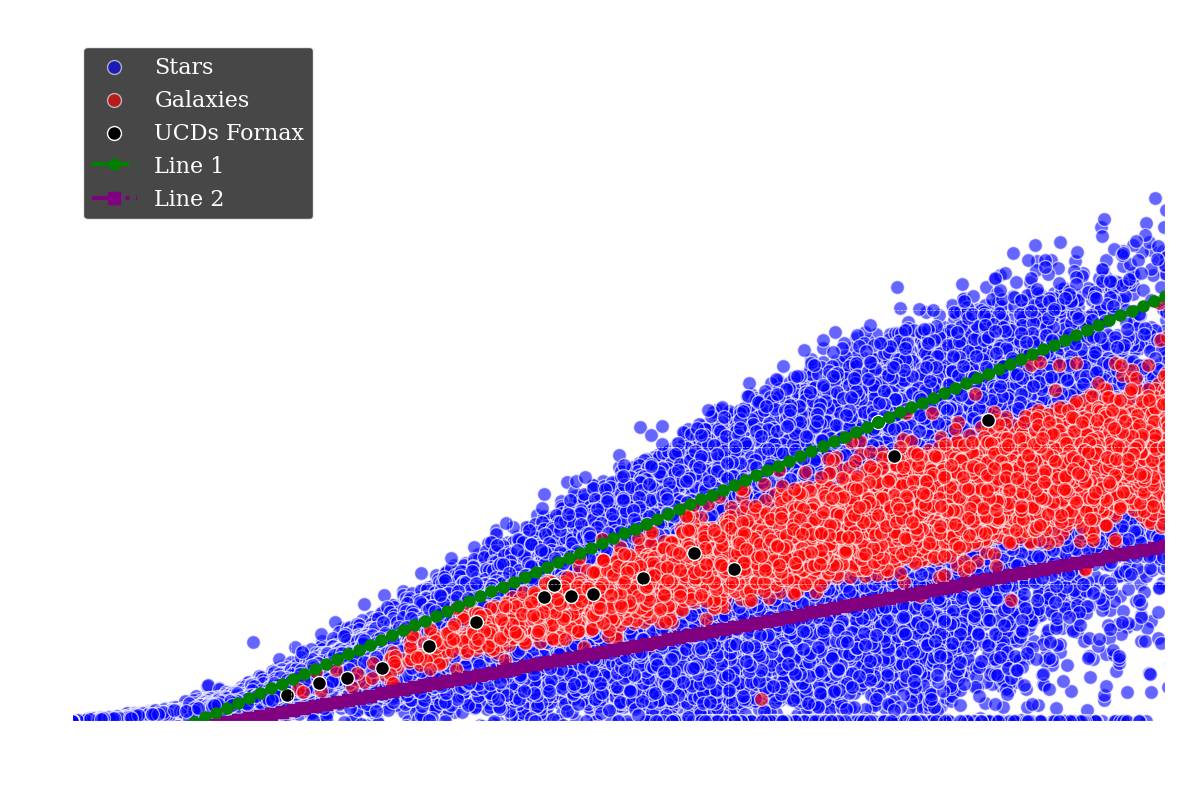
\includegraphics[width=\linewidth]{images/f_90_70_FLUX_RADIUS_90_R.png}
        \end{figure}
    \end{column}
    \begin{column}{0.32\linewidth}
        \begin{figure}
            \centering
            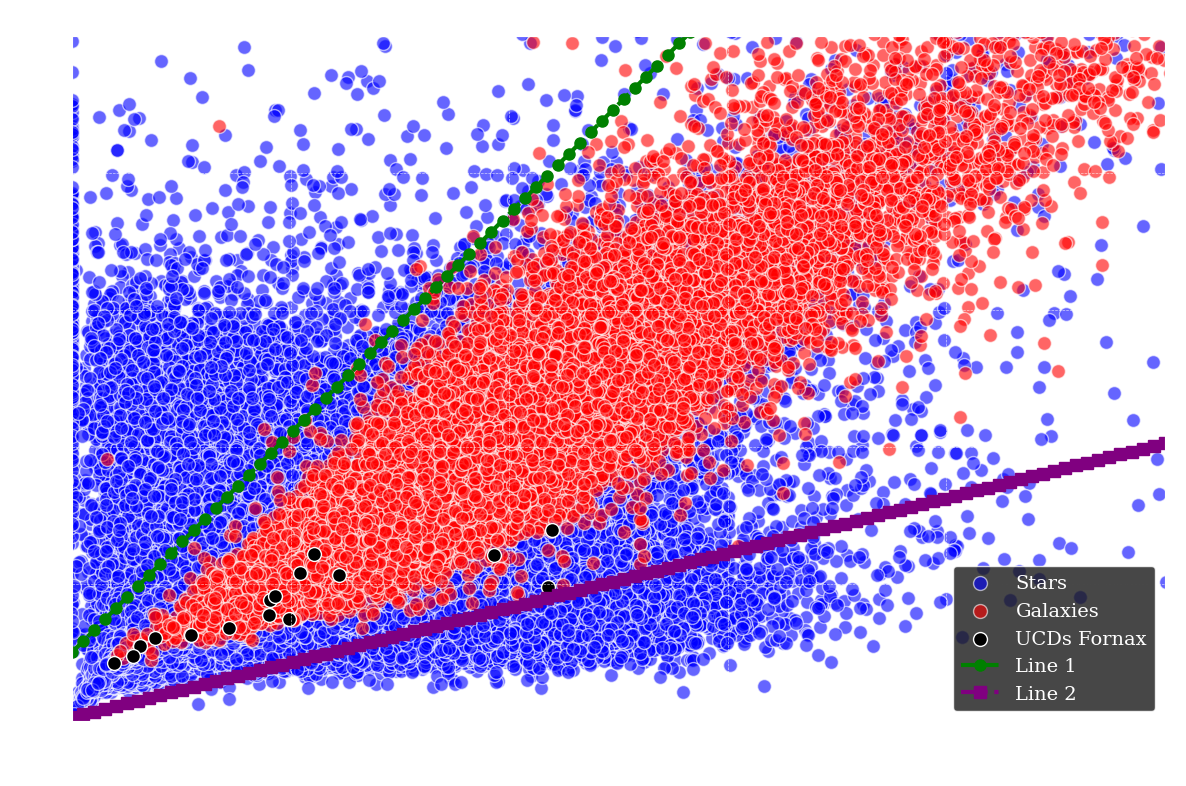
\includegraphics[width=\linewidth]{images/f_70_20_f_90_70.png}
        \end{figure}
    \end{column}
\end{columns}

\begin{center}
    \footnotesize
    \textbf{Total de objetos selecionados: 242.}
\end{center}

\end{frame}

\begin{frame}[c]{Seleção das candidatas}
\scriptsize
Seleção com S-PLUS e classificações GAIA

Seleção final: 14 candidatas
\begin{columns}[c]
        \begin{column}{0.48\textwidth}
            \begin{figure}
                \centering
                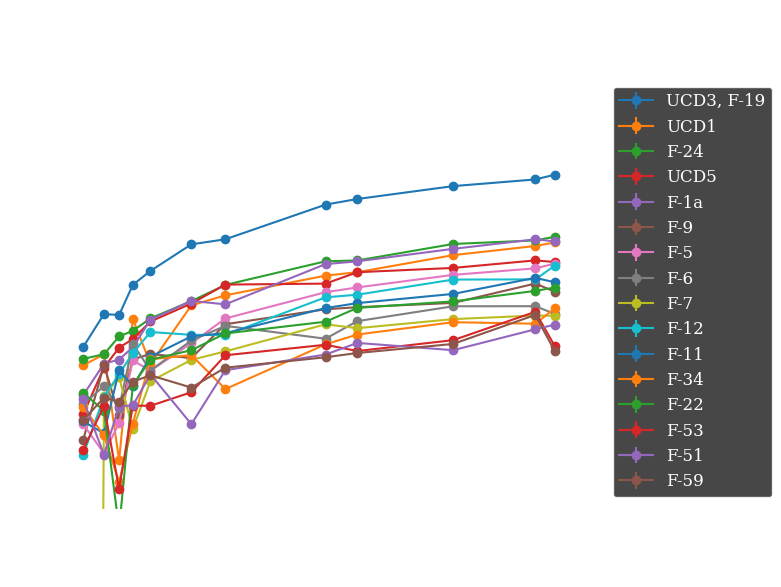
\includegraphics[width=\textwidth]{images/photospec_ucds.png}
            \end{figure}
        \end{column}
        \begin{column}{0.48\textwidth}
            \begin{figure}
                \centering
                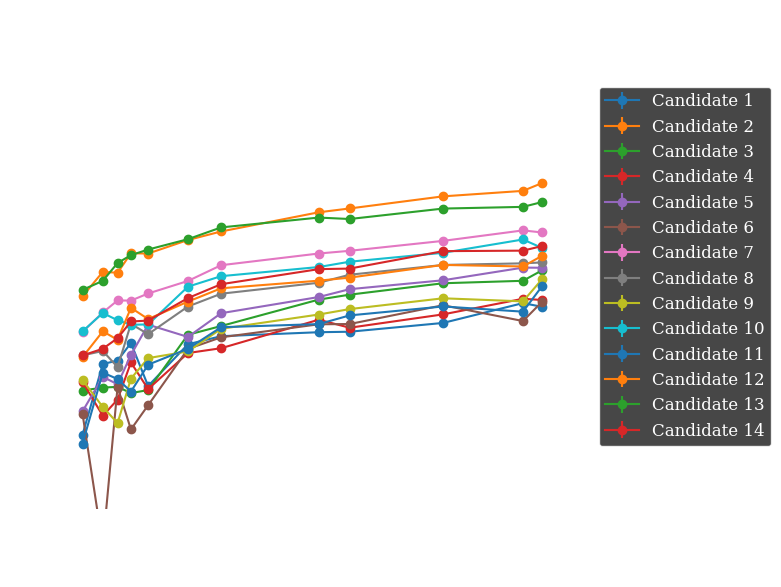
\includegraphics[width=\textwidth]{images/photospec_candidatas.png}
            \end{figure}
        \end{column}
    \end{columns}
\end{frame}

\begin{frame}[c]{Seleção das candidatas}
    \begin{figure}[]
        \captionsetup{justification=centering}
        \begin{subfigure}[b]{0.13\textwidth}
            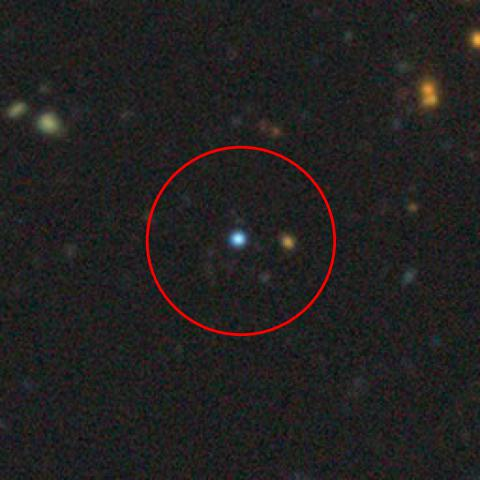
\includegraphics[width=\textwidth]{images/candidata_final/01.jpg}
            \caption{Candidate 01}
        \end{subfigure}
        \begin{subfigure}[b]{0.13\textwidth}
            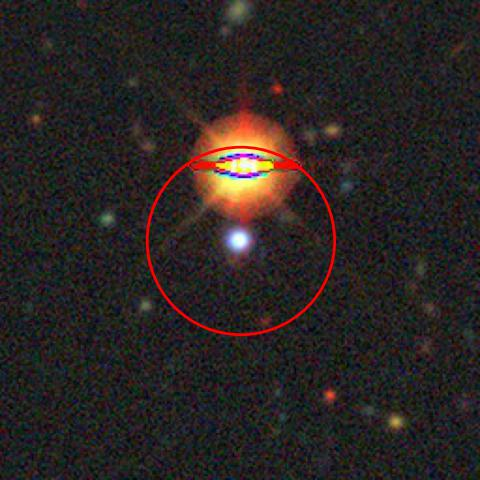
\includegraphics[width=\textwidth]{images/candidata_final/02.jpg}
            \caption{Candidate 02}
        \end{subfigure}
        \begin{subfigure}[b]{0.13\textwidth}
            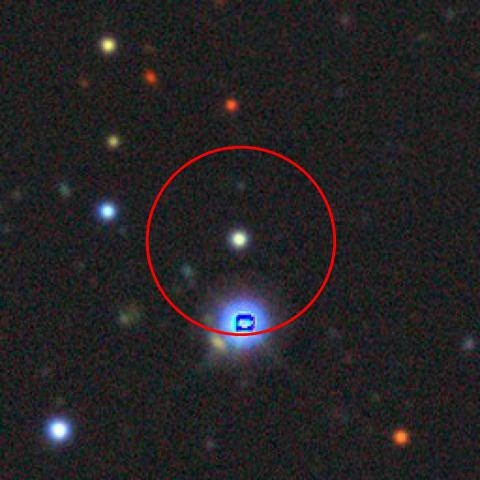
\includegraphics[width=\textwidth]{images/candidata_final/03.jpg}
            \caption{Candidate 03}
        \end{subfigure}
        \begin{subfigure}[b]{0.13\textwidth}
            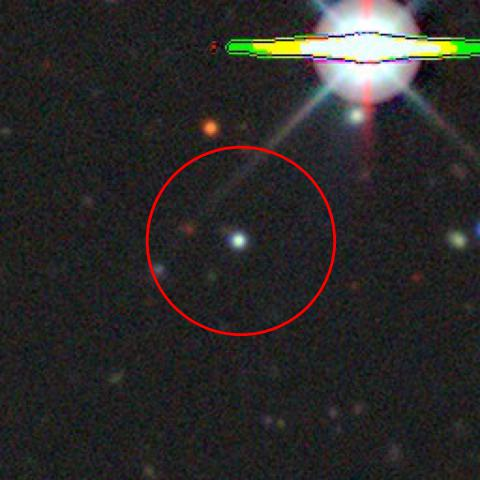
\includegraphics[width=\textwidth]{images/candidata_final/04.jpg}
            \caption{Candidate 04}
        \end{subfigure}
        \begin{subfigure}[b]{0.13\textwidth}
            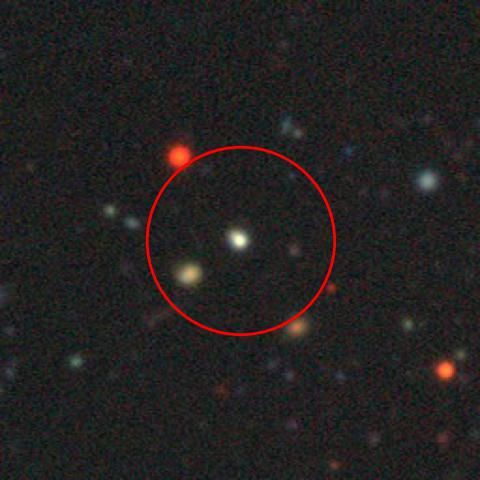
\includegraphics[width=\textwidth]{images/candidata_final/05.jpg}
            \caption{Candidate 05}
        \end{subfigure}
        \begin{subfigure}[b]{0.13\textwidth}
            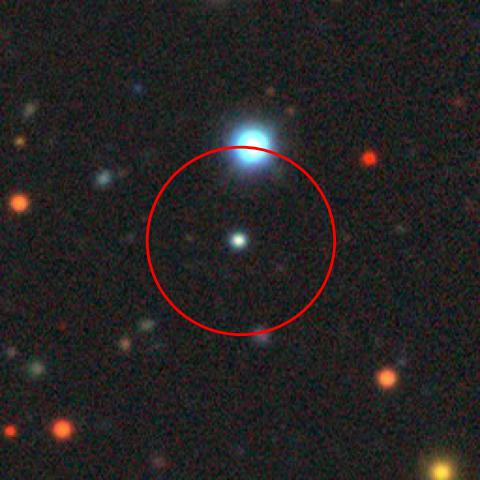
\includegraphics[width=\textwidth]{images/candidata_final/06.jpg}
            \caption{Candidate 06}
        \end{subfigure}
        \begin{subfigure}[b]{0.13\textwidth}
            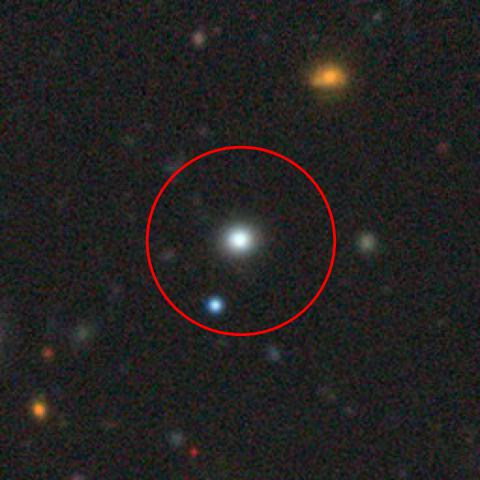
\includegraphics[width=\textwidth]{images/candidata_final/07.jpg}
            \caption{Candidate 07}
        \end{subfigure}
        \begin{subfigure}[b]{0.13\textwidth}
            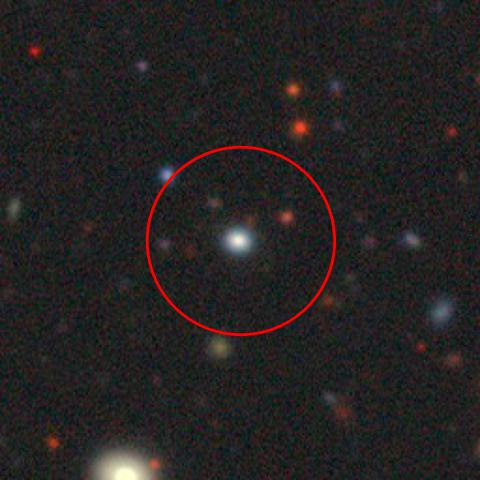
\includegraphics[width=\textwidth]{images/candidata_final/08.jpg}
            \caption{Candidate 08}
        \end{subfigure}
        \begin{subfigure}[b]{0.13\textwidth}
            \includegraphics[width=\textwidth]{images/candidata_final/09.jpg}
            \caption{Candidate 09}
        \end{subfigure}
        \begin{subfigure}[b]{0.13\textwidth}
            \includegraphics[width=\textwidth]{images/candidata_final/10.jpg}
            \caption{Candidate 10}
        \end{subfigure}
        \begin{subfigure}[b]{0.13\textwidth}
            \includegraphics[width=\textwidth]{images/candidata_final/11.jpg}
            \caption{Candidate 11}
        \end{subfigure}
        \begin{subfigure}[b]{0.13\textwidth}
            \includegraphics[width=\textwidth]{images/candidata_final/12.jpg}
            \caption{Candidate 12}
        \end{subfigure}
        \begin{subfigure}[b]{0.13\textwidth}
            \includegraphics[width=\textwidth]{images/candidata_final/13.jpg}
            \caption{Candidate 13}
        \end{subfigure}
        \begin{subfigure}[b]{0.13\textwidth}
            \includegraphics[width=\textwidth]{images/candidata_final/14.jpg}
            \caption{Candidate 14}
        \end{subfigure}
    \end{figure}
\end{frame}

\begin{frame}[c]{Análise das candidatas}
\small
\textbf{Catálogo Fornax (Castelli et al. 2024)}

\begin{figure}
    \includegraphics[width=\paperwidth,height=0.9\paperheight,keepaspectratio]{images/analise_junta.png}
\end{figure}

\end{frame}


\begin{frame}[c]{Análise das candidatas}
\small
\textbf{Distribuição em Fornax}

\begin{figure}
    \centering
    \includegraphics[width=1.\linewidth]{images/candidates_distribution.png}
\end{figure}

\end{frame}

\begin{frame}[c]{Conclusões sobre as candidatas UCDs}
    \begin{itemize}
        \item Apenas 1 das 14 candidatas está dentro do raio viral de Fornax;
        \item As candidatas selecionadas apresentam características compatíveis com UCDs conhecidas.
        \item Presença em regiões periféricas sugere que UCDs podem se formar em ambientes menos densos e migrar para o centro posteriormente.
        \item Múltiplos cenários de formação possíveis:
        \begin{itemize}
            \item Fusão de superaglomerados estelares em regiões de menor densidade.
            \item Colapso direto de nuvens de gás primordial.
            \item Stripping de galáxias anãs nucleadas em ambientes densos.
        \end{itemize}
        \item Resultados reforçam a hipótese de múltiplos canais de formação para UCDs.
        \item Descoberta de UCDs fora do raio viral amplia o conhecimento sobre sua distribuição e mecanismos de formação.
    \end{itemize}
\end{frame}

\section{Observações espectroscópicas Candidatas UCDs}

\begin{frame}[c]{Observações espectroscópicas}
Amostra de candidatas a UCDs ({\scriptsize Projeto IC anterior})
\vspace{-0.3cm}
\begin{figure}
    \captionsetup{justification=centering}
    \centering
    \begin{subfigure}[b]{0.11\textwidth}
        \includegraphics[width=\textwidth]{images/proposatal_candidatas_1/UCG01.png}
        \caption{Candidate 01}
    \end{subfigure}
    \begin{subfigure}[b]{0.11\textwidth}
        \includegraphics[width=\textwidth]{images/proposatal_candidatas_1/UCG02.png}
        \caption{Candidate 02}
    \end{subfigure}
    \begin{subfigure}[b]{0.11\textwidth}
        \includegraphics[width=\textwidth]{images/proposatal_candidatas_1/UCG03.jpg}
        \caption{Candidate 03}
    \end{subfigure}
    \begin{subfigure}[b]{0.11\textwidth}
        \includegraphics[width=\textwidth]{images/proposatal_candidatas_1/UCG04.jpg}
        \caption{Candidate 04}
    \end{subfigure}
    \begin{subfigure}[b]{0.11\textwidth}
        \includegraphics[width=\textwidth]{images/proposatal_candidatas_1/UCG05.jpg}
        \caption{Candidate 05}
    \end{subfigure}
    \begin{subfigure}[b]{0.11\textwidth}
        \includegraphics[width=\textwidth]{images/proposatal_candidatas_1/UCG06.jpg}
        \caption{Candidate 06}
    \end{subfigure}
    \begin{subfigure}[b]{0.11\textwidth}
        \includegraphics[width=\textwidth]{images/proposatal_candidatas_1/UCG07.jpg}
        \caption{Candidate 07}
    \end{subfigure}
    \begin{subfigure}[b]{0.11\textwidth}
        \includegraphics[width=\textwidth]{images/proposatal_candidatas_1/UCG08.jpg}
        \caption{Candidate 08}
    \end{subfigure}
    \begin{subfigure}[b]{0.11\textwidth}
        \includegraphics[width=\textwidth]{images/proposatal_candidatas_1/UCG09.jpg}
        \caption{Candidate 09}
    \end{subfigure}
    \begin{subfigure}[b]{0.11\textwidth}
        \includegraphics[width=\textwidth]{images/proposatal_candidatas_1/UCG10.jpg}
        \caption{Candidate 10}
    \end{subfigure}
    \begin{subfigure}[b]{0.11\textwidth}
        \includegraphics[width=\textwidth]{images/proposatal_candidatas_1/UCG11.jpg}
        \caption{Candidate 11}
    \end{subfigure}
    \begin{subfigure}[b]{0.11\textwidth}
        \includegraphics[width=\textwidth]{images/proposatal_candidatas_1/UCG12.jpg}
        \caption{Candidate 12}
    \end{subfigure}
    \begin{subfigure}[b]{0.11\textwidth}
        \includegraphics[width=\textwidth]{images/proposatal_candidatas_1/UCG13.jpg}
        \caption{Candidate 13}
    \end{subfigure}
    \begin{subfigure}[b]{0.11\textwidth}
        \includegraphics[width=\textwidth]{images/proposatal_candidatas_1/UCG14.jpg}
        \caption{Candidate 14}
    \end{subfigure}
    \begin{subfigure}[b]{0.11\textwidth}
        \includegraphics[width=\textwidth]{images/proposatal_candidatas_1/UCG15.jpg}
        \caption{Candidate 15}
    \end{subfigure}
    \begin{subfigure}[b]{0.11\textwidth}
        \includegraphics[width=\textwidth]{images/proposatal_candidatas_1/UCG16.jpg}
        \caption{Candidate 16}
    \end{subfigure}
    \begin{subfigure}[b]{0.11\textwidth}
        \includegraphics[width=\textwidth]{images/proposatal_candidatas_1/UCG17.jpg}
        \caption{Candidate 17}
    \end{subfigure}
    \begin{subfigure}[b]{0.11\textwidth}
        \includegraphics[width=\textwidth]{images/proposatal_candidatas_1/UCG18.jpg}
        \caption{Candidate 18}
    \end{subfigure}
\end{figure}
\end{frame}

\begin{frame}[c]{Observações espectroscópicas}
Observações com o Gemini Sul
\footnotesize
\begin{itemize}
    \item \textbf{Modo de Observação}: Fenda longa (\textit{long-slit}).
    \item \textbf{Grating}: B600-G5303, com comprimento de onda central $\lambda_c = 550 \, \text{nm}$.
    \item \textbf{Largura da Fenda}: 1,5".
    \item \textbf{Resolução Espectral}: $R \sim 570$, considerando a largura da fenda escolhida.
    \item \textbf{Intervalo Espectral}: 4000\,\text{Å} a 7000\,\text{Å}, cobrindo desde o azul até quase o vermelho.
    \item \textbf{Tempo de Exposição por Objeto}: 1200 segundos, divididos em 3 exposições de 400 segundos cada.
    \item \textbf{Condições de Observação}: IQ=ANY, CC=80\%, WV=ANY, SB=ANY.
    \item \textbf{Razão Sinal-Ruído (S/N) Desejada}: Mínimo de 5 no espectro combinado (equivalente a S/N $\sim$ 3 por pixel espectral) no contínuo, suficiente para detectar o declive do contínuo azul e as principais linhas de absorção.
\end{itemize}

{\scriptsize Não foram observadas as candidatas UCG04, UCG09, UCG11, e UCG17.}
\end{frame}

\begin{frame}[c]{Observações espectroscópicas}
\textbf{Fluxo de Redução dos Dados Espectroscópicos}

\begin{enumerate}
    \item \textbf{Seleção dos dados:} Escolha dos frames científicos e de calibração.
    \item \textbf{Remoção do bias:} Subtração do bias para eliminar o sinal eletrônico de fundo.
    \item \textbf{Correção de flat-field:} Correção da resposta pixel a pixel do detector usando imagens de flat.
    \item \textbf{Calibração em comprimento de onda:} Utilização de lâmpadas de arco para calibrar o eixo espectral.
    \item \textbf{Correção de resposta espectral:} Processamento dos dados da estrela padrão para correção da resposta instrumental e do fluxo.
    \item \textbf{Redução dos dados científicos:} Aplicação das correções e calibrações aos espectros dos objetos de interesse.
\end{enumerate}

\end{frame}

\begin{frame}[c]{Observações espectroscópicas}
\begin{figure}
    \captionsetup{justification=centering}
    \centering
    \begin{subfigure}[b]{0.31\textwidth}
        \includegraphics[width=\textwidth]{images/espectros/UCG01.png}
        \caption{Candidate 01}
    \end{subfigure}
    \begin{subfigure}[b]{0.31\textwidth}
        \includegraphics[width=\textwidth]{images/espectros/UCG02.png}
        \caption{Candidate 02}
    \end{subfigure}
    \begin{subfigure}[b]{0.31\textwidth}
        \includegraphics[width=\textwidth]{images/espectros/UCG03.png}
        \caption{Candidate 03}
    \end{subfigure}
    \begin{subfigure}[b]{0.31\textwidth}
        \includegraphics[width=\textwidth]{images/espectros/UCG05.png}
        \caption{Candidate 05}
    \end{subfigure}
    \begin{subfigure}[b]{0.31\textwidth}
        \includegraphics[width=\textwidth]{images/espectros/UCG06.png}
        \caption{Candidate 06}
    \end{subfigure}
    \begin{subfigure}[b]{0.31\textwidth}
        \includegraphics[width=\textwidth]{images/espectros/UCG07.png}
        \caption{Candidate 07}
    \end{subfigure}
\end{figure}
\end{frame}

\begin{frame}[c]{Observações espectroscópicas}
\begin{figure}
    \captionsetup{justification=centering}
    \centering
    \begin{subfigure}[b]{0.31\textwidth}
        \includegraphics[width=\textwidth]{images/espectros/UCG08.png}
        \caption{Candidate 08}
    \end{subfigure}
    \begin{subfigure}[b]{0.31\textwidth}
        \includegraphics[width=\textwidth]{images/espectros/UCG10.png}
        \caption{Candidate 10}
    \end{subfigure}
    \begin{subfigure}[b]{0.31\textwidth}
        \includegraphics[width=\textwidth]{images/espectros/UCG12.png}
        \caption{Candidate 12}
    \end{subfigure}
    \begin{subfigure}[b]{0.31\textwidth}
        \includegraphics[width=\textwidth]{images/espectros/UCG13.png}
        \caption{Candidate 13}
    \end{subfigure}
    \begin{subfigure}[b]{0.31\textwidth}
        \includegraphics[width=\textwidth]{images/espectros/UCG14.png}
        \caption{Candidate 14}
    \end{subfigure}
    \begin{subfigure}[b]{0.31\textwidth}
        \includegraphics[width=\textwidth]{images/espectros/UCG15.png}
        \caption{Candidate 15}
    \end{subfigure}
\end{figure}
\end{frame}

\begin{frame}[c]{Observações espectroscópicas}
\begin{figure}
    \captionsetup{justification=centering}
    \centering
    \begin{subfigure}[b]{0.31\textwidth}
        \includegraphics[width=\textwidth]{images/espectros/UCG16.png}
        \caption{Candidate 16}
    \end{subfigure}
    \begin{subfigure}[b]{0.31\textwidth}
        \includegraphics[width=\textwidth]{images/espectros/UCG18.png}
        \caption{Candidate 18}
    \end{subfigure}
\end{figure}
\end{frame}

\begin{frame}[c]{Observações espectroscópicas}
\begin{columns}[c]
    \begin{column}{0.52\textwidth}
        \begin{table}[!ht]
            \centering
            \footnotesize
            \begin{tabular}{lcc}
                \toprule
                $OBJ_{name}$ & z   \\
                \midrule
                UCG01     & 0.0005 \\
                UCG02     & 0.0004 \\
                UCG03     & 0.147 \\
                UCG05     & 0.02 \\
                UCG06     & -0.0003 \\
                UCG07     & -0.0003 \\
                UCG08     & -0.0001 \\
                UCG10     & 2.48 \\
                UCG12     & 0.0995 \\
                UCG13     & 0.0004 \\
                UCG14     & 0.027 \\
                UCG15     & 0.0006 \\
                UCG16     & 0.0004 \\
                UCG18     & 0.039 \\
                \bottomrule
            \end{tabular}
            \label{redshift_candidatas_1}
        \end{table}
    \end{column}
    \begin{column}{0.48\textwidth}
        \small
        Temos 9 classificados como estrelas (UCG01, UCG02, UCG06, UCG07, UCG08, UCG13, UCG15, UCG16), 1 como quasar (UCG10) e 5 como galáxias (UCG03, UCG05, UCG12, UCG14, UCG18). Das galáxias encontradas nessa amostra, nenhuma foi classificada como pertencente ao aglomerado de Fornax.
    \end{column}
\end{columns}
\end{frame}

\section{Objetos compactos com emissão}

\begin{frame}[c]{Objetos compactos com emissão}
Seleção de objetos compactos com sinais de linhas de emissão

Identificação de objetos compactos azuis com evidências de linhas de emissão, como as Blue Compact Dwarf Galaxies (BCDs).

As linhas de emissão mais sensíveis ao filtro $J0660$ do S-PLUS são H$\alpha$ e [OIII].

A seleção foi realizada buscando objetos compactos com emissão em H$\alpha$ e/ou [OIII], utilizando o excesso de fluxo no filtro $J0660$ em relação aos filtros adjacentes.

\begin{splusbox}{Seleção baseada em cor H$\alpha$}
    \begin{equation}
        \text{Color}_{\mathrm{H}\alpha} = J0660 - \frac{r + i}{2}
        \label{equation_halpha_color}
    \end{equation}
    Objetos com $\text{Color}_{\mathrm{H}\alpha}$ significativamente negativos indicam emissão em H$\alpha$.
\end{splusbox}

\end{frame}

\begin{frame}[c]{Objetos compactos com emissão}
Seleção de objetos compactos com emissão
\vspace{-0.5cm}
\begin{figure}[h]
    \centering
    \captionsetup{justification=centering}
    \begin{subfigure}[b]{0.25\textwidth}
        \includegraphics[width=\textwidth]{images/photo_specs/Candidate_1.png}
        \caption{Candidate\_1}
    \end{subfigure}
    \begin{subfigure}[b]{0.25\textwidth}
        \includegraphics[width=\textwidth]{images/photo_specs/Candidate_2.png}
        \caption{Candidate\_2}
    \end{subfigure}
    \begin{subfigure}[b]{0.25\textwidth}
        \includegraphics[width=\textwidth]{images/photo_specs/Candidate_3.png}
        \caption{Candidate\_3}
    \end{subfigure}
    \begin{subfigure}[b]{0.25\textwidth}
        \includegraphics[width=\textwidth]{images/photo_specs/Candidate_4.png}
        \caption{Candidate\_4}
    \end{subfigure}
    \begin{subfigure}[b]{0.25\textwidth}
        \includegraphics[width=\textwidth]{images/photo_specs/Candidate_5.png}
        \caption{Candidate\_5}
    \end{subfigure}
    \begin{subfigure}[b]{0.25\textwidth}
        \includegraphics[width=\textwidth]{images/photo_specs/Candidate_6.png}
        \caption{Candidate\_6}
    \end{subfigure}
\end{figure}

\end{frame}

\begin{frame}[c]{Objetos compactos com emissão}
\begin{figure}[h]
    \centering
    \captionsetup{justification=centering}
    \begin{subfigure}[b]{0.22\textwidth}
        \includegraphics[width=\textwidth]{images/proposatal_candidatas_2/Candidate_1.png}
        \caption{Candidate\_1}
    \end{subfigure}
    \begin{subfigure}[b]{0.22\textwidth}
        \includegraphics[width=\textwidth]{images/proposatal_candidatas_2/Candidate_2.png}
        \caption{Candidate\_2}
    \end{subfigure}
    \begin{subfigure}[b]{0.22\textwidth}
        \includegraphics[width=\textwidth]{images/proposatal_candidatas_2/Candidate_3.png}
        \caption{Candidate\_3}
    \end{subfigure}
\end{figure}
\vspace{-0.5cm}
\begin{figure}[h]
    \begin{subfigure}[b]{0.22\textwidth}
        \includegraphics[width=\textwidth]{images/proposatal_candidatas_2/Candidate_4.png}
        \caption{Candidate\_4}
    \end{subfigure}
    \begin{subfigure}[b]{0.22\textwidth}
        \includegraphics[width=\textwidth]{images/proposatal_candidatas_2/Candidate_5.png}
        \caption{Candidate\_5}
    \end{subfigure}
    \begin{subfigure}[b]{0.22\textwidth}
        \includegraphics[width=\textwidth]{images/proposatal_candidatas_2/Candidate_6.png}
        \caption{Candidate\_6}
    \end{subfigure}
\end{figure}

\end{frame}


\begin{frame}[c]{Observações espectroscópicas}
Observações com o Gemini Sul (Fast Turn Around Program)
\footnotesize
\begin{itemize}
    \item \textbf{Modo de Observação}: Fenda longa (\textit{long-slit}).
    \item \textbf{Grating}: B600-G5323, com comprimento de onda central em 3 posições: $\lambda_c = 515 \, \text{nm}$, $\lambda_c = 550 \, \text{nm}$ e $\lambda_c = 585 \, \text{nm}$.
    \item \textbf{Largura da Fenda}: 1".
    \item \textbf{Resolução Espectral}: $R \sim 570$, considerando a largura da fenda escolhida.
    \item \textbf{Intervalo Espectral}: 4000\,\text{Å} a 7000\,\text{Å}.
    \item \textbf{Condições de Observação}: IQ=85\%, CC=70\%, WV=ANY, SB=80\%.
    \item \textbf{Razão Sinal-Ruído (S/N) Desejada}: Mínimo de 3 no espectro combinado no contínuo, suficiente para detectar o declive do contínuo azul e as principais linhas de absorção.
    \item \textbf{Número de Exposições}: Em cada comprimento de onda central, 1 exposição de 600 segundos cada, totalizando 3 exposições por objeto.
\end{itemize}

\end{frame}

\begin{frame}[c]{Observações espectroscópicas}
\vspace{0.1cm}
\begin{figure}
    \captionsetup{justification=centering}
    \centering
    \begin{subfigure}[b]{0.31\textwidth}
        \includegraphics[width=\textwidth]{images/espectros/Candidate1.png}
        \caption{Candidate 01}
    \end{subfigure}
    \begin{subfigure}[b]{0.31\textwidth}
        \includegraphics[width=\textwidth]{images/espectros/Candidate2.png}
        \caption{Candidate 02}
    \end{subfigure}
    \begin{subfigure}[b]{0.31\textwidth}
        \includegraphics[width=\textwidth]{images/espectros/Candidate3.png}
        \caption{Candidate 03}
    \end{subfigure}
    \begin{subfigure}[b]{0.31\textwidth}
        \includegraphics[width=\textwidth]{images/espectros/Candidate4.png}
        \caption{Candidate 05}
    \end{subfigure}
    \begin{subfigure}[b]{0.31\textwidth}
        \includegraphics[width=\textwidth]{images/espectros/Candidate5.png}
        \caption{Candidate 06}
    \end{subfigure}
    \begin{subfigure}[b]{0.31\textwidth}
        \includegraphics[width=\textwidth]{images/espectros/Candidate6.png}
        \caption{Candidate 07}
    \end{subfigure}
\end{figure}
\end{frame}

\begin{frame}[c]{Resultados compact emission galaxies}
\begin{columns}[c]
    \begin{column}{0.45\textwidth}
        \begin{table}[h]
            \centering
            \begin{tabular}{lcc}
                \toprule
                $OBJ_{name}$ & z   \\
                \midrule
                Candidate\_1     & 0.309 \\
                Candidate\_2     & 0.265 \\
                Candidate\_3     & 0.327 \\
                Candidate\_4     & 0.323 \\
                Candidate\_5     & 0.308 \\
                Candidate\_6     & 0.325 \\
                \bottomrule
            \end{tabular}
        \end{table}
    \end{column}
    \begin{column}{0.55\textwidth}
        \vspace{0.3cm}
        \begin{itemize}
            \item Todos os objetos apresentam sinais de emissão bem definidos.
            \item Espectros mostram objetos azuis, com formação estelar recente e linhas de emissão intensas.
            \item Redshifts entre 0.265 e 0.327: objetos estão distantes do aglomerado de Fornax.
            \item Mesmo compactos, os objetos apresentam fortes linhas de emissão, indicando formação estelar recente.
            \item Método eficiente para encontrar galáxias compactas com emissão em $z \sim 0.3$.
        \end{itemize}
    \end{column}
\end{columns}
\end{frame}

\section{Conclusões e perspectivas}

\begin{frame}[c]{Conclusões}
    \scriptsize
    \begin{columns}[t]
        \begin{column}{0.48\textwidth}
            \begin{splusbox}{Busca por UCDs em Fornax}
                \begin{itemize}
                    \item Busca sistemática por galáxias anãs ultra-compactas (UCDs) no aglomerado de Fornax, integrando:
                    \begin{itemize}
                        \scriptsize
                        \item Análises fotométricas e morfológicas
                        \item Aprendizado de máquina (Random Forest: AUC-ROC 0.97, MCC 0.84)
                        \item Observações espectroscópicas (Gemini Sul)
                    \end{itemize}
                    \item Seleção de 14 novas candidatas principais a UCDs, com propriedades compatíveis com UCDs conhecidas.
                    \item Candidatas apresentam distribuição espacial periférica.
                    \item Metodologia eficaz e replicável para identificação de UCDs em outros levantamentos.
                \end{itemize}
            \end{splusbox}
        \end{column}
        \begin{column}{0.48\textwidth}
            \begin{splusbox}{Objetos Compactos com Emissão}
                \begin{itemize}
                    \item Metodologia também eficiente para identificar galáxias compactas emissoras (possíveis BCDs).
                    \item Inclusão de cortes envolvendo o filtro $J0660$ pode refinar futuras buscas.
                    \item Estratégia baseada em aprendizado de máquina e critérios fotométricos/morfológicos mostrou-se robusta.
                \end{itemize}
            \end{splusbox}
        \end{column}
    \end{columns}
\end{frame}

\begin{frame}[c]{Perspectivas e próximos passos}
    \begin{itemize}
        \item Solicitação de tempo de observação espectroscópica para confirmar a natureza das novas candidatas a UCDs.
        \item Observações futuras serão fundamentais para validar propriedades morfológicas e fotométricas, além de fornecer informações adicionais sobre composição e dinâmica.
        \item Metodologia pode ser aplicada e expandida para outros campos, levantamentos e aglomerados próximos (ex: Hydra).
        \item Explorar cenários de formação e evolução das UCDs em ambientes menos densos e incluir modelos que considerem crescimento contínuo e eventos de \textit{infall} tardio.
        \item Busca por objetos compactos com emissão também mostrou-se promissora, podendo ser aplicada em regiões com redshift mais elevado.
    \end{itemize}
\end{frame}

\begin{frame}[c]
    \centering
    \vspace{2cm}
    {\LARGE \textbf{Obrigado!}}
\end{frame}

% \begin{frame}[c]{Redshifts Fotométricos}

% \begin{frame}[c]{Redshifts Fotométricos}
%     \begin{columns}[c]
%         \begin{column}{0.32\linewidth}
%             \begin{figure}
%                 \centering
%                 \includegraphics[width=\linewidth]{images/results_scatterplot_residuals.pdf}
%                 \caption{Resíduos entre $z_\text{phot}$ e $z_\text{spec}$.}
%             \end{figure}
%         \end{column}
%         \begin{column}{0.32\linewidth}
%             \begin{figure}
%                 \centering
%                 \includegraphics[width=\linewidth]{images/results_spe_metrics.pdf}
%                 \caption{Métricas de desempenho do modelo.}
%             \end{figure}
%         \end{column}
%         \begin{column}{0.32\linewidth}
%             \begin{figure}
%                 \centering
%                 \includegraphics[width=\linewidth]{images/results_pdf_metrics_triangle.pdf}
%                 \caption{Distribuição das PDFs geradas.}
%             \end{figure}
%         \end{column}
%     \end{columns}
% \end{frame}

% % Slide 8: Conclusões
% \begin{frame}[c]{Conclusões}
%     \begin{splusbox}{Resumo}
%         \begin{itemize}
%             \item Modelo RF apresentou melhor desempenho em comparação ao KNN.
%             \item Classificação baseada em FWHM é eficiente para separar objetos compactos e extensos.
%             \item Tratamento de valores faltantes foi essencial para garantir consistência nos resultados.
%         \end{itemize}
%     \end{splusbox}
% \end{frame}

% \section{aaaa}
% \begin{frame}[c]{Criando o catálogo para treinamento}
%     \begin{splusbox}{Crossmatches espectroscópicos}
%         \small
%         Busca radial (RA, DEC) com raio de 2" em torno de cada objeto do SPLUS
%     \end{splusbox}
%     \begin{splusbox}{Crossmatches fotométricos}
%         \small
%         \begin{columns}[t]
%             \begin{column}{0.29\textwidth}
%                GALEX \textcolor{LightGray}{(II/335/galex\_ais)}:
%                \begin{itemize}
%                     \item Busca radial com raio de 2"
%                 \end{itemize}
%             \end{column}
%             \begin{column}{0.29\textwidth}
%                 VHS \textcolor{LightGray}{(II/367/vhs\_dr5)}:
%                 \begin{itemize}
%                     \justifying
%                     \item Busca radial com raio de 1"
%                     \item Conversão de magnitudes Vega para AB
%                 \end{itemize}
%             \end{column}
%             \begin{column}{0.29\textwidth}
%                 unWISE \textcolor{LightGray}{(II/363/unwise)}:
%                 \begin{itemize}
%                     \justifying
%                     \item Busca radial com raio de 1"
%                     \item Cálculo das magnitudes e erros
%                     \item Conversão de magnitudes Vega para AB
%                 \end{itemize}
%             \end{column}
%         \end{columns}
%     \end{splusbox}
% \end{frame}

% \begin{frame}[c]{Pré-processamento}
%     \begin{columns}[c]
%         \begin{column}{0.56\linewidth}
%             \vspace{0.2cm}
%             \begin{table}
%                 \centering
%                 \label{tab:constraints}
%                   \begin{tabular}{@{}ll@{}}
%                       \toprule
%                       \textbf{Variable}        & \textbf{Constraints}                              \\ \midrule
%                       \texttt{r\_auto}         & {[}14, 21{]}                                      \\
%                       \texttt{nDet\_PStotal}   & $\geqslant$ 1                                     \\
%                       \texttt{SEX\_FLAGS\_DET} & {[}0, 3{]}                                        \\ \midrule
%                       \texttt{z}               & {[}0.002, 0.8{]}                                    \\
%                       \texttt{e\_z}            & $\leqslant$ 0.002                                 \\
%                       \texttt{f\_z}            & not \ttt{REMOVE}                                  \\
%                       \texttt{class\_spec}     & \ttt{GALAXY}, \ttt{SUPERNOVAE} or \ttt{AGN}       \\
%                       Separation               & $\leqslant$ 1''                                   \\ \bottomrule
%                   \end{tabular}
%               \end{table}
%         \end{column}
%         %
%         %\hspace*{-2cm}
%         \begin{column}{0.36\linewidth}
%             \begin{splusbox}{}
%                 \begin{itemize}
%                     \justifying
%                     \item Galáxias
%                     \item Nem muito fracas, nem muito brilhantes
%                     \item Com boa fotometria
%                     \item Com redshifts de boa qualidade e entre 0.002 e 0.8
%                 \end{itemize}
%             \end{splusbox}
%         \end{column}
%     \end{columns}
% \end{frame}

% \begin{frame}[c]{Pré-processamento}
%     \begin{figure}
%         \centering
%         \includegraphics[height=7cm]{script/images/constraints_effect.pdf}
%     \end{figure}
% \end{frame}

% \begin{frame}[c]{Pesos por objeto}
%     A distribuição de spec-zs da amostra de treino é diferente da distribuição esperada no universo.
%     \begin{equation*}
%         P(y|\mathcal{D}) = \int P(y,\theta|\mathcal{D}) \text{d}\theta = \int P(y|\theta, \mathcal{D}) P(\theta|D) \text{d}\theta
%     \end{equation*}
%     % \hspace{0.5cm}
%     \begin{splusbox}{}
%         Os resultados para $y$ dependem dos dados $\mathcal{D}$, então o conjunto de treinamento pode introduzir viéses.
%     \end{splusbox}
% \end{frame}

% \begin{frame}[c]{Pesos por objeto}
%     Assumimos que a distribuição de $z_\text{spec}$ é conhecida para surveys limitados por fluxo, e modelamos esta distribuição como função da magnitude usando a amostra do COSMOS2020 (Weaver et al., 2022) e uma função Weibull de dois parâmetros $l$ e $k$.

%     \begin{figure}
%         \centering
%         \includegraphics[width=\linewidth]{script/images/laerte_fit.pdf}
%     \end{figure}
% \end{frame}

% \begin{frame}[c]{Pesos por objeto}
%     \begin{figure}
%         \centering
%         \includegraphics[width=\linewidth]{script/images/weights_vs_specz.pdf}
%     \end{figure}

%     Com essa abordagem, cada objeto contribui de forma diferente no treinamento do modelo
% \end{frame}

% \section{Metodologia}
%     % \begin{tikzpicture}[overlay, remember picture]
%     %     % Image 1 at specified position
%     %     \node at (3.75, 1.5) {\includegraphics[height=4cm]{script/images/neuron_bio.png}};
        
%     %     % Image 2 at specified position
%     %     \node at (11, -1.5) {\includegraphics[height=4cm]{script/images/neuron_bio.png}};
%     % \end{tikzpicture}

% \begin{frame}[c]{Redes neurais}
%     \begin{figure}
%         \centering
%         \includegraphics[height=6cm]{script/images/neuron_bio.png}
%     \end{figure}
% \end{frame}

% \begin{frame}[c]{Redes neurais}
%     \begin{figure}
%         \centering
%         \includegraphics[height=6cm]{script/images/neuron_ml_pesos.png}
%     \end{figure}
% \end{frame}

% % \begin{frame}[c]{Redes neurais}
% %     \begin{figure}
% %         \centering
% %         \includegraphics[height=6cm]{script/images/rede_normal.png}
% %     \end{figure}
% % \end{frame}

% \begin{frame}[c]{Redes neurais Bayesianas}
%     \begin{figure}
%         \centering
%         \includegraphics[height=6cm]{script/images/neuron_ml_bayes.png}
%     \end{figure}
% \end{frame}

% \begin{frame}[c]{Redes de mistura de densidades}
%     \begin{figure}
%         \centering
%         \includegraphics[height=6cm]{script/images/rede_mdn.png}
%     \end{figure}
% \end{frame}

% \begin{frame}[c]{Redes de mistura de densidades}
%     \begin{figure}
%         \centering
%         \includegraphics[width=\linewidth]{script/images/mixture_pdf_5comp.pdf}
%     \end{figure}
% \end{frame}

% \begin{frame}[c]{Redes de mistura de densidades Bayesiana}
%     Usamos uma combinação da abordagem Bayesiana com a de mistura de densidades, criando uma rede cujos pesos são distribuições e que, como saida, fornece $N$ componentes de uma mistura de densidades.

%     \begin{columns}[c]
%         \begin{column}{0.46\textwidth}
%             \begin{splusbox}{Bayesian Neural Network}
%                 \begin{itemize}
%                     \item Modelagem de incertezas
%                     \begin{itemize}
%                         \item Aleatória (dos dados)
%                         \item Epistêmica (do modelo)
%                     \end{itemize}
%                 \end{itemize}
%             \end{splusbox}
%         \end{column}
%         \begin{column}{0.46\textwidth}
%             \begin{splusbox}{Mixture Density Network}
%                 \begin{itemize}
%                     \item Gera PDFs bem calibradas diretamente, inteiramente descritas por poucos parâmetros
%                     \item É eficiente em termos de armazenamento
%                 \end{itemize}
%             \end{splusbox}
%         \end{column}
%     \end{columns}

%     % \begin{itemize}
%     %     \justifying
%     %     \item A abordagem Bayesiana permite que a rede leve em conta incertezas inerentes do problema, como aquelas devido à medição da fotometria (aleatória) e das estimativas do modelo (epistêmica).
%     %     \item É capaz de produzir funções de densidade de probabilidade (PDFs) de forma natural e direta, sendo que estas são calibradas durante o treinamento do modelo.
%     % \end{itemize}
% \end{frame}

% \section{Definindo a arquitetura}
% \begin{frame}[c]{Definindo a arquitetura da rede com o \texttt{Optuna}}
%     \begin{figure}
%         \centering
%         \includegraphics[width=\linewidth]{script/images/optuna_metrics_scatter.pdf}
%     \end{figure}
% \end{frame}

% % \begin{frame}[c]{Definindo a arquitetura da rede com o \texttt{Optuna}}
% %     \begin{columns}[c]
% %         \small
% %         \begin{column}{0.49\textwidth}
% %             \begin{splusbox}{Parâmetros para amostrar}
% %                 Para cada abertura do SPLUS:
% %                 \begin{itemize}
% %                     \item Camadas: 3 a 6
% %                     \item Neurônios por camada: 64 a 128
% %                     \item Função de ativação: leakyrelu, relu, elu, gelu, selu, prelu, rrelu, silu, mish, celu
% %                     \item Viés nas camadas: Verdadeiro ou Falso
% %                     \item Camada de atenção por feature: Verdadeiro ou falso
% %                     \item Learning rate: 0.001 a 0.03
% %                     \item Weight decay: 0.000001 a 0.0001
% %                     \item Otimizador: adam, nadam, adamw, adabelief, ranger
% %                 \end{itemize}
% %             \end{splusbox}
% %         \end{column}
% %         \begin{column}{0.49\textwidth}
% %             \begin{splusbox}{Parâmetros escolhidos}
% %                 Abertura PStotal
% %                 \begin{itemize}
% %                     \item Camadas: 4
% %                     \item Neurônios: 64
% %                     \item Função de ativação: gelu
% %                     \item Viés nas camadas: Verdadeiro
% %                     \item Camada de atenção por feature: Verdadeiro
% %                     \item Learning rate: 0.0296
% %                     \item Weight decay: $7.5 \times 10^{-6}$
% %                     \item Otimizador: adabelief
% %                 \end{itemize}
% %             \end{splusbox}
% %         \end{column}
% %     \end{columns}
% % \end{frame}

% \begin{frame}[c]{Definindo a arquitetura da rede com o \texttt{Optuna}}
%     \begin{table}
%         \centering
%           \begin{tabular}{@{}lll@{}}
%               \toprule
%               \textbf{Variável}   & \textbf{Parâmetros para amostrar}     & \textbf{Parâmetros escolhidos} \\ \midrule
%               Camadas             & 3 a 6                                 & 4                              \\
%               Neurônios           & 64 a 128                              & 64                             \\
%               Ativação            & Todas as "\texttt{LU}"                  & \texttt{gelu}                  \\
%               Otimizador          & Variações de \texttt{Adam}            & \texttt{AdaBelief}             \\
%               Learning rate       & 0.001 a 0.03                          & 0.0296                         \\
%               Weight decay        & $1 \times 10^{-6}$ a $1 \times 10^{-4}$ & $7.5 \times 10^{-6}$           \\
%               Viés das camadas    & \texttt{True} ou \texttt{False}       & \texttt{True}                  \\
%               Atenção por feature & \texttt{True} ou \texttt{False}       & \texttt{True}                  \\ \bottomrule
%           \end{tabular}
%       \end{table}

%       \begin{tcolorbox}
%           Em todos os casos, os valores de entrada foram   magnitudes, cores e informações morfológicas
%       \end{tcolorbox}
% \end{frame}

% \section{Resultados}
% % \begin{frame}[c]{Redshifts fotométricos: estimativas de ponto único}
% %     \begin{itemize}
% %         \item $\sigma_\text{NMAD}$:
% %         \begin{equation*}
% %             \sigma_\text{NMAD} = 1.48 \times \text{mediana} \left( \left| \frac{{\delta z} - \text{mediana}(\delta z)}{1+z_\text{spec}} \right| \right)
% %         \end{equation*}
% %         \item Bias ($\mu$):
% %         \begin{align*}
% %             \mu &= \text{mediana} \left( \delta z \right), \\
% %             \mu_\text{norm} &= \text{mediana} \left( \frac{\delta z}{1+z_{\text{spec}}} \right).
% %         \end{align*}
% %         \item Fração de outliers ($\eta$):
% %         \begin{align*}
% %             \eta &= \frac{|\delta z|}{1+z_\text{spec}} > 0.15, \\
% %             \eta_{N\sigma} &= \frac{|\delta z|}{1+z_\text{spec}} > N \cdot \sigma_\text{NMAD}.
% %         \end{align*}
% %     \end{itemize}
% % \end{frame}

% \begin{frame}[c]{Redshifts fotométricos: estimativas de ponto único}
%     \begin{splusbox}{Desvio médio absoluto normalizado ($\sigma_\text{NMAD}${, \textcolor{LightGray}{Brammer et al., 2008}})}
%         \begin{equation*}
%             \sigma_\text{NMAD} = 1.48 \times \text{mediana} \left( \left| \frac{{\delta z} - \text{mediana}(\delta z)}{1+z_\text{spec}} \right| \right)
%         \end{equation*}
%     \end{splusbox}

%     % \begin{splusbox}{Desvio médio absoluto normalizado ($\sigma_\text{NMAD}$)}
%     %     \vspace{-.5cm}
%     %     \begin{columns}[c]
%     %         \begin{column}{0.58\textwidth}
%     %             \centering
%     %             \begin{equation*}
%     %                 \sigma_\text{NMAD} = 1.48 \times \text{mediana} \left( \left| \frac{{\delta z} - \text{mediana}(\delta z)}{1+z_\text{spec}} \right| \right)
%     %             \end{equation*}
%     %         \end{column}
%     %         \begin{column}{0.38\textwidth}
%     %             \centering
%     %             \begin{equation*}
%     %                 \delta z = z_\text{phot} - z_\text{spec}
%     %             \end{equation*}
%     %         \end{column}
%     %     \end{columns}
%     % \end{splusbox}

%     \begin{splusbox}{Viés ($\mu$)}
%         \vspace{-.5cm}
%         \begin{columns}[c]
%             \begin{column}{0.46\textwidth}
%                 \centering
%                 \begin{equation*}
%                     \mu = \text{mediana} \left( \delta z \right)
%                 \end{equation*}
%             \end{column}
%             \begin{column}{0.46\textwidth}
%                 \centering
%                 \begin{equation*}
%                     \mu_\text{norm} = \text{mediana} \left( \frac{\delta z}{1+z_{\text{spec}}} \right)
%                 \end{equation*}
%             \end{column}
%             \hspace*{1cm}
%         \end{columns}
%     \end{splusbox}

%     \begin{splusbox}{Fração de outliers ($\eta${, {\textcolor{LightGray}{Ilbert et al., 2006; Dahlen et al., 2013}}})}
%         \vspace{-.5cm}
%         \begin{columns}[c]
%             \begin{column}{0.46\textwidth}
%                 \centering
%                 \begin{equation*}
%                     \eta = \frac{|\delta z|}{1+z_\text{spec}} > 0.15
%                 \end{equation*}
%             \end{column}
%             \begin{column}{0.46\textwidth}
%                 \centering
%                 \begin{equation*}
%                     \eta_{N\sigma} = \frac{|\delta z|}{1+z_\text{spec}} > N \cdot \sigma_\text{NMAD}
%                 \end{equation*}
%             \end{column}
%             \hspace*{1cm}
%         \end{columns}
%     \end{splusbox}
% \end{frame}

% \begin{frame}[c]{Redshifts fotométricos: estimativas de ponto único}
%     \begin{figure}
%         \centering
%         \includegraphics[height=7cm]{script/images/results_scatterplot_residuals.pdf}
%     \end{figure}
% \end{frame}

% \begin{frame}[c]{Redshifts fotométricos: estimativas de ponto único}
%     \begin{figure}
%         \centering
%         \includegraphics[height=7cm]{script/images/results_spe_metrics.pdf}
%     \end{figure}
% \end{frame}

% \begin{frame}[c]{Redshifts fotométricos: estimativas de ponto único}
%     \begin{figure}
%         \centering
%         \includegraphics[width=\linewidth]{script/images/results_spe_metrics_2d.pdf}
%     \end{figure}
% \end{frame}

% \begin{frame}[c]{Redshifts fotométricos: estimativas de ponto único}
%     Para verificar se a distribuição de photo-zs está como é esperado, comparamos os resultados que obtemos com os resultados de dois outros modelos, um KNN e uma RF, para objetos na Stripe-82.

%     \begin{figure}
%         \centering
%         \includegraphics[width=0.8\linewidth]{script/images/s82_redshifts.pdf}
%     \end{figure}
% \end{frame}

% \begin{frame}[c]{Redshifts fotométricos: funções de densidade de probabilidade}
%     % \begin{itemize}
%     %     \item Odds \textcolor{LightGray}{(Benitez, 2000)}
%     %     \item Highest Probability Density Credible Interval \textcolor{LightGray}{(Wittman et al., 2016)}
%     %     \item Probability Integral Transform \textcolor{LightGray}{(Polsterer et al., 2016)}
%     %     %\item Continuous Ranked Probability Score \textcolor{LightGray}{(Hersbach, 2000; Polsterer et al., 2016)}
%     %     \item $\sigma_{68}$ e valor máximo
%     % \end{itemize}

%     \begin{splusbox}{Odds \textcolor{LightGray}{(Benitez, 2000)}}
%         \small
%         \vspace{-.5cm}
%         \begin{align*}
%           \text{odds}_i = \int_{z_\text{peak, $i$}-\Delta z}^{z_\text{peak, $i$}+\Delta z} \text{PDF}_i(z)~\text{d}z,
%         \end{align*}
%     \end{splusbox}

%     \begin{splusbox}{Probability Integral Transform \textcolor{LightGray}{(Polsterer et al., 2016)}}
%         \small
%         \vspace{-.5cm}
%         \begin{align*}
%             \text{PIT}_i = \int_{0}^{z_\text{spec}} \text{PDF}_i(z)~\text{d}z = \text{CDF}_i(z_\text{spec}).
%           \end{align*}
%     \end{splusbox}

%     \centering
%     \begin{tcolorbox}[hbox]
%         \small
%         Highest Probability Density Credible Interval \textcolor{LightGray}{(Wittman et al., 2016)}
%     \end{tcolorbox}

%     \begin{tcolorbox}[hbox]
%         \small
%         $\sigma_{68}$ e valor máximo
%     \end{tcolorbox}

% \end{frame}

% \begin{frame}[c]{Redshifts fotométricos: funções de densidade de probabilidade}
%     \begin{figure}
%         \centering
%         \includegraphics[height=7cm]{script/images/results_pdf_metrics_illust_2.pdf}
%     \end{figure}
% \end{frame}

% % \begin{frame}[c]{Redshifts fotométricos: funções de densidade de probabilidade}
% %     PDF: apresentar métricas, histogramas de calibração, resultados por campo
% % \end{frame}

% \begin{frame}[c]{Redshifts fotométricos: funções de densidade de probabilidade}
%     \begin{figure}
%         \centering
%         \includegraphics[height=7cm]{script/images/result_pdf_summary.pdf}
%     \end{figure}
% \end{frame}

% \begin{frame}[c]{Redshifts fotométricos: funções de densidade de probabilidade}
%     \begin{figure}
%         \centering
%         \includegraphics[width=\linewidth]{script/images/results_pdf_metrics_2d.pdf}
%     \end{figure}
% \end{frame}

% \section{Estrutura em larga escala}
% \begin{frame}[c]{Estrutura em larga escala}
%     \begin{figure}
%         \centering
%         \includegraphics[width=\linewidth]{script/images/lss_problem.pdf}
%     \end{figure}
%     %
%     \centering
%     \begin{tcolorbox}[hbox] % <---
%         Interpretamos que o $z_\text{phot}$ é igual a $z_\text{spec} + \epsilon$
%     \end{tcolorbox}
%     % \begin{splusbox}{}
%     %     \centering
%     %     Interpretamos que o $z_\text{phot}$ é igual a $z_\text{spec} + \epsilon$
%     % \end{splusbox}
% \end{frame}

% % \begin{frame}[c]{Estrutura em larga escala}
% %     \begin{splusbox}{Autoencoders e U-Nets}
% %         Redes desenvolvidas especificamente para fazer compressão de dados, podendo remover ruído
% %     \end{splusbox}

% %     \begin{splusbox}{Denoising Diffusion Probabilistic Models (DDPMs)}
% %         Redes que utilizam um processo de difusão (e difusão inversa) para aprender uma distribuição que representa os dados, podem ser utilizadas para remover ruído
% %     \end{splusbox}

% %     \begin{splusbox}{Graph Neural Networks (GNNs)}
% %         Redes que utilizam outra estrutura de dados (grafos), e que é capaz de utilizar informação de posição e relação entre amostras para melhorar seus resultados
% %     \end{splusbox}
% % \end{frame}

% \begin{frame}[c]{Estrutura em larga escala}
%     \centering
%     % \begin{splusbox}{}
%     %     \large Autoencoders e U-Nets
%     % \end{splusbox}

%     % \begin{splusbox}{}
%     %     \large Denoising Diffusion Probabilistic Models (DDPMs)
%     % \end{splusbox}

%     % \begin{splusbox}{}
%     %     \large Graph Neural Networks (GNNs)
%     % \end{splusbox}

%     \begin{tcolorbox}[hbox] % <---
%         \large Autoencoders e U-Nets
%     \end{tcolorbox}
%     \vspace{0.5cm}
%     \begin{tcolorbox}[hbox] % <---
%         \large Denoising Diffusion Probabilistic Models (DDPMs)
%     \end{tcolorbox}
%     \vspace{0.5cm}
%     \begin{tcolorbox}[hbox] % <---
%         \large Graph Neural Networks (GNNs)
%     \end{tcolorbox}
% \end{frame}

% \begin{frame}[c]{Autoencoders {\small \textcolor{LightGray}{(Kramer, 1991; Kingma e Welling, 2013; Ronnerberger et al., 2015)}}}
%     \begin{columns}[c]
%         \begin{column}{0.36\linewidth}
%             \begin{splusbox}{}
%                 \begin{itemize}
%                     \justifying
%                     \item São caracterizadas pela existência de um gargalo
%                     \item Treinamento simultâneo de duas redes
%                     \item Tem como objetivo reproduzir o input com menos informação
%                     \item Remove ruído pois ele não é fundamental na reconstrução do input
%                 \end{itemize}
%             \end{splusbox}
%         \end{column}
%         \begin{column}{0.56\linewidth}
%             \begin{figure}
%                 \centering
%                 \includegraphics[height=6.5cm]{script/images/autoencoders.png}
%             \end{figure}
%         \end{column}
%     \end{columns}
% \end{frame}

% \begin{frame}[c]{Autoencoders}
%     \begin{figure}
%         \centering
%         \includegraphics[width=\linewidth]{script/images/redshift_polar_plot_zml_zmlae_zmlvae.pdf}
%     \end{figure}
% \end{frame}

% \begin{frame}[c]{Autoencoders}
%     \begin{figure}
%         \centering
%         \includegraphics[height=7cm]{script/images/2pcf_compare_corrfunc.pdf}
%     \end{figure}
% \end{frame}

% \begin{frame}[c]{Denoising Diffusion Probabilistic Models  {\small \textcolor{LightGray}{(Ho et al., 2020)}}}
%     \begin{figure}
%         \centering
%         \includegraphics[width=\linewidth]{script/images/diffusion.png}
%         \caption{Adaptado de \url{https://cvpr2022-tutorial-diffusion-models.github.io/}.}
%     \end{figure}

%     \centering
%     \begin{splusbox}{}
%         É capaz de modelar as incertezas sem suposições simples (por ex. erros são Gaussianos), e pode aprender correlações nas incertezas do photo-z
%     \end{splusbox}
%     % \begin{tcolorbox}[hbox]
%     %     É capaz de modelar as incertezas sem suposições simples (por ex. erros são Gaussianos), e pode aprender correlações nas incertezas do photo-z
%     % \end{tcolorbox}
% \end{frame}

% % \begin{frame}[c]{Denoising Diffusion Probabilistic Models}
% %     \begin{splusbox}{}
% %         \begin{itemize}
% %             \item Modelagem das incertezas como um forward-process
% %             \item É capaz de aprender correlações e efeitos não-Gaussianos nas incertezas do photo-z
% %             %\item Condicionamento na fotometria, permitindo a obtenção de um photo-z mais próximo ao spec-z diretamente, contornando a necessidade de passos intermediários
% %             \item Fornece estimativas probabilísticas
% %         \end{itemize}
% %     \end{splusbox}
% % \end{frame}

% \begin{frame}[c]{Denoising Diffusion Probabilistic Models}
%     \begin{columns}[c]
%         \begin{column}{0.46\linewidth}
%             \begin{splusbox}{Tabular}
%                 \begin{itemize}
%                     \item[$\checkmark$] Lida com a estrutura natural dos dados
%                     \item[$\checkmark$] Computacionalmente mais leve
%                     \item[$\times$] Sem possibilidade de aprender relações espaciais
%                     \item[$\times$] Não usa arquiteturas comuns a esse problema
%                 \end{itemize}
%             \end{splusbox}
%         \end{column}
%         \begin{column}{0.46\linewidth}
%             \begin{splusbox}{Imagens}
%                 \begin{itemize}
%                     \item[$\checkmark$] Usa arquiteturas conhecidas (U-Net)
%                     \item[$\checkmark$] Aprenderia relações espaciais
%                     \item[$\checkmark$] Entendimento mais simples
%                     \item[$\times$] Computacionalmente mais pesado
%                     \item[$\times$] Modifica a forma natural dos dados
%                 \end{itemize}
%             \end{splusbox}
%         \end{column}
%     \end{columns}
% \end{frame}

% \begin{frame}[c]{Denoising Diffusion Probabilistic Models}
%     \begin{figure}
%         \centering
%         \includegraphics[width=\linewidth]{script/images/lss_illustration.pdf}
%     \end{figure}
%     %
%     \begin{splusbox}{}
%         \begin{itemize}
%             \item O ruído é modelado de forma que partimos de $z_\text{spec}$ e chegamos em $z_\text{phot}$
%             \item O modelo é condicionado na fotometria, dispensando a necessidade de saber o timestep $t$
%         \end{itemize}
%     \end{splusbox}
% \end{frame}

% \begin{frame}[c]{Denoising Diffusion Probabilistic Models}
%     \begin{figure}
%         \centering
%         \includegraphics[height=7cm]{script/images/ddpm_diffusion_features.pdf}
%     \end{figure}
% \end{frame}

% \begin{frame}[c]{Denoising Diffusion Probabilistic Models}
%     \begin{figure}
%         \centering
%         \includegraphics[height=7cm]{script/images/ddpm_diffusion_z.pdf}
%     \end{figure}
% \end{frame}

% \begin{frame}[c]{Graph Neural Networks {\small \textcolor{LightGray}{(Gori et al., 2005; Scarselli et al., 2009)}}}
%     \begin{columns}[c]
%         \begin{column}{0.46\linewidth}
%             \begin{splusbox}{}
%                 \begin{itemize}
%                     \justifying
%                     \item Sistemas de recomendação
%                     \item Detecção de fraudes
%                     \item Descoberta de medicamentos
%                     \item Identificação de estruturas de proteínas
%                     \item Otimização de cadeias de produção
%                 \end{itemize}
%             \end{splusbox}
%         \end{column}
%         \begin{column}{0.46\linewidth}
%             \begin{figure}
%                 \centering
%                 \includegraphics[height=5.5cm]{images/planetoidcora.png}
%                 \caption{Adaptado de \url{https://graphsandnetworks.com/the-cora-dataset/}}
%             \end{figure}
%         \end{column}
%     \end{columns}
% \end{frame}

% \begin{frame}[c]{Graph Neural Networks}
%     \begin{figure}
%         \centering
%         \includegraphics[height=7cm]{images/galaxy_graph.pdf}
%     \end{figure}
% \end{frame}

% \begin{frame}[c]{Graph Neural Networks}
%     \begin{figure}
%         \centering
%         \includegraphics[height=7cm]{images/galaxy_graph_gnn.pdf}
%     \end{figure}
% \end{frame}

% \begin{frame}[c]{Graph Neural Networks}
%     \begin{figure}
%         \centering
%         \includegraphics[width=0.9\linewidth]{images/gnn_message.png}
%         \caption{Adaptado de \url{https://snap.stanford.edu/graphsage/}.}
%     \end{figure}
% \end{frame}

% % \begin{frame}[c]{Graph Neural Networks {\small \textcolor{LightGray}{(Gori et al., 2005; Scarselli et al., 2009)}}}
% %     \begin{figure}
% %         \centering
% %         \includegraphics[width=\linewidth]{script/images/sample_and_agg.png}
% %         \caption{Adaptado de \url{https://snap.stanford.edu/graphsage/}}
% %     \end{figure}
% % \end{frame}

% % \begin{frame}[c]{Graph Neural Networks}
% %     \begin{figure}
% %         \centering
% %         \includegraphics[height=7cm]{script/images/gnn.png}
% %     \end{figure}
% % \end{frame}

% % \begin{frame}[c]{Estrutura em larga escala}
% %     \begin{figure}
% %         \centering
% %         \includegraphics[height=7cm]{script/images/redshift_polar_plot_z_zml.pdf}
% %     \end{figure}
% % \end{frame}

% \section{Conclusões}
% % \begin{frame}[c]{Conclusões}
% %     \begin{splusbox}{Redshifts fotométricos}
% %         \begin{itemize}
% %             %\item A estimativa de redshifts fotométricos é fundamental para diversos casos científicos
% %             \item O nosso modelo faz estimativas pontuais precisas e acuradas
% %             \item Fornece funções de densidade de probabilidade bem calibradas
% %             \item Geramos um catálogo com essas informações para toda a colaboração
% %         \end{itemize}
% %     \end{splusbox}
% % \end{frame}

% % \begin{frame}[c]{Conclusões}
% %     \begin{splusbox}{Redshifts espectroscópicos}
% %         \begin{itemize}
% %             \item Criamos o maior compilado de redshifts espectroscópicos do Hemisfério Sul
% %         \end{itemize}
% %     \end{splusbox}

% %     \begin{splusbox}{Estrutura em larga escala}
% %         \begin{itemize}
% %             \item A precisão dos $z_\text{phot}$s serve como ponto de partida para a etapa de recuperação da LSS
% %             \item Identificamos possíveis caminhos de progresso (DDPMs, GNNs)
% %             \item Este trabalho ainda está em andamento
% %         \end{itemize}
% %     \end{splusbox}
% % \end{frame}

% \begin{frame}[c]{Conclusões}
%     \small
%     \vspace*{0.2cm}
%     \begin{splusbox}{Redshifts fotométricos}
%         \begin{itemize}
%             \setlength\itemsep{.1em}
%             %\item A estimativa de redshifts fotométricos é fundamental para diversos casos científicos
%             \item O nosso modelo faz estimativas pontuais precisas e acuradas
%             \item Fornece funções de densidade de probabilidade bem calibradas
%             \item Geramos um catálogo com essas informações para toda a colaboração
%         \end{itemize}
%     \end{splusbox}
    
%     \begin{splusbox}{Redshifts espectroscópicos}
%         \begin{itemize}
%             \setlength\itemsep{.1em}
%             \item Criamos o maior compilado de redshifts espectroscópicos do Hemisfério Sul
%         \end{itemize}
%     \end{splusbox}

%     \begin{splusbox}{Estrutura em larga escala}
%         \begin{itemize}
%             \setlength\itemsep{.1em}
%             \item A precisão dos $z_\text{phot}$s serve como ponto de partida para a etapa de recuperação da LSS
%             \item Identificamos possíveis caminhos de progresso (DDPMs, GNNs)
%             \item Este trabalho ainda está em andamento
%         \end{itemize}
%     \end{splusbox}
% \end{frame}

% \section{Perspectivas futuras}
% \begin{frame}[c]{Perspectivas futuras}
%     \begin{splusbox}{Redshifts fotométricos}
%         \small
%         \begin{itemize}
%             \item Refatoração do código de forma a simplificá-lo e torná-lo mais eficiente
%             \item Desenvolvimento de um código aberto no qual qualquer usuário tem acesso aos modelos e pode fazer estimativas por conta
%             \item Aprimoração dos modelos
%             \begin{itemize}
%                 \item Uso de distribuição de magnitudes como input para o treino do modelo
%                 %\item Criar uma opção de predição determinística
%                 \item Implementação de uma etapa de template-fitting no processo de treinamento
%                 %\item Criação de um ensemble
%                 \item Arquitetura no estilo Mixture-of-Experts/Transformer
%             \end{itemize}
%         \end{itemize}
%     \end{splusbox}
% \end{frame}

% %\setlength\itemsep{1em}

% \begin{frame}[c]{Perspectivas futuras}
%     \begin{splusbox}{Compilado espectroscópico}
%         \small
%         \begin{itemize}
%             \item Criar uma nova versão do código que faz o compilado de $z_\text{spec}$, que seja eficiente e fácil de compreender, para divulgação à comunidade.
%         \end{itemize}
%     \end{splusbox}

%     \begin{splusbox}{Estrutura em larga escala}
%         \small
%         \begin{itemize}
%             \item Continuidade nas pesquisas relacionadas à reconstrução da LSS explorando DDPMs e GNNs
%             %\item Exploração das metodologias de DDPMs e GNNs, pois ambas apresentam grande potencial para o nosso objetivo
%             \item Obtenção da estrutura da LSS reconstruída
%             \item Utilizar este resultado como ponto de partida para outras pesquisas
%         \end{itemize}
%     \end{splusbox}
% \end{frame}

% \usebeamertemplate{endpage}

% \appendix

% \section{Slides extras}

% \begin{frame}[c]{Definindo a arquitetura da rede com o \texttt{Optuna}}
%     \begin{figure}
%         \centering
%         \includegraphics[height=7cm]{script/images/optuna_metrics_boxplots.pdf}
%     \end{figure}
% \end{frame}

% \begin{frame}[c]{Redshifts fotométricos: funções de densidade de probabilidade}
%     \begin{figure}
%         \centering
%         \includegraphics[height=7cm]{script/images/odds_vs_odds_norm.pdf}
%     \end{figure}
% \end{frame}

% \begin{frame}[c]{Redshifts fotométricos: funções de densidade de probabilidade}
%     \begin{figure}
%         \centering
%         \includegraphics[height=7cm]{script/images/results_pdf_average.pdf}
%     \end{figure}
% \end{frame}

% \begin{frame}[c]{Redshifts fotométricos: funções de densidade de probabilidade}
%     \begin{figure}
%         \centering
%         \includegraphics[height=7cm]{script/images/results_pdf_odds_mag_and_z.pdf}
%     \end{figure}
% \end{frame}

% \begin{frame}[c]{Redshifts fotométricos: funções de densidade de probabilidade}
%     \begin{figure}
%         \centering
%         \includegraphics[height=7cm]{script/images/results_pdf_hpdci_mag_z.pdf}
%     \end{figure}
% \end{frame}

% \begin{frame}[c]{Redshifts fotométricos: funções de densidade de probabilidade}
%     \begin{figure}
%         \centering
%         \includegraphics[height=7cm]{script/images/results_pdf_pit_mag_and_z.pdf}
%     \end{figure}
% \end{frame}

% \begin{frame}[c]{Redshifts fotométricos: funções de densidade de probabilidade}
%     \begin{figure}
%         \centering
%         \includegraphics[height=7cm]{script/images/results_pdf_metrics_triangle.pdf}
%     \end{figure}
% \end{frame}